\documentclass[a4paper,11pt]{report}
\usepackage{xr}
\usepackage[utf8]{inputenc}
\usepackage{graphicx}
\usepackage{caption}
\usepackage{subcaption}
\usepackage{scrextend}
\usepackage[english]{babel}
\usepackage[vmargin=3.5cm, top=2cm]{geometry}
\usepackage[linktocpage=true]{hyperref}
\usepackage{enumitem}
\usepackage{longtable}
\usepackage{pdfpages}
\usepackage[font=small,labelfont=bf]{caption}
\usepackage{float}
\usepackage{hyperref}
\usepackage[section]{placeins}
\usepackage{listings}
\usepackage{url}
\urlstyle{same}
\hypersetup{
    colorlinks,
    citecolor=black,
    filecolor=black,
    linkcolor=black,
    urlcolor=black
}
\newcommand{\tmtable}{\begin{longtable}{ p{2.7cm} p{10cm} }}
\newcommand{\tmtableend}{\end{longtable}}
\renewcommand{\baselinestretch}{1.0} 

\begin{document}
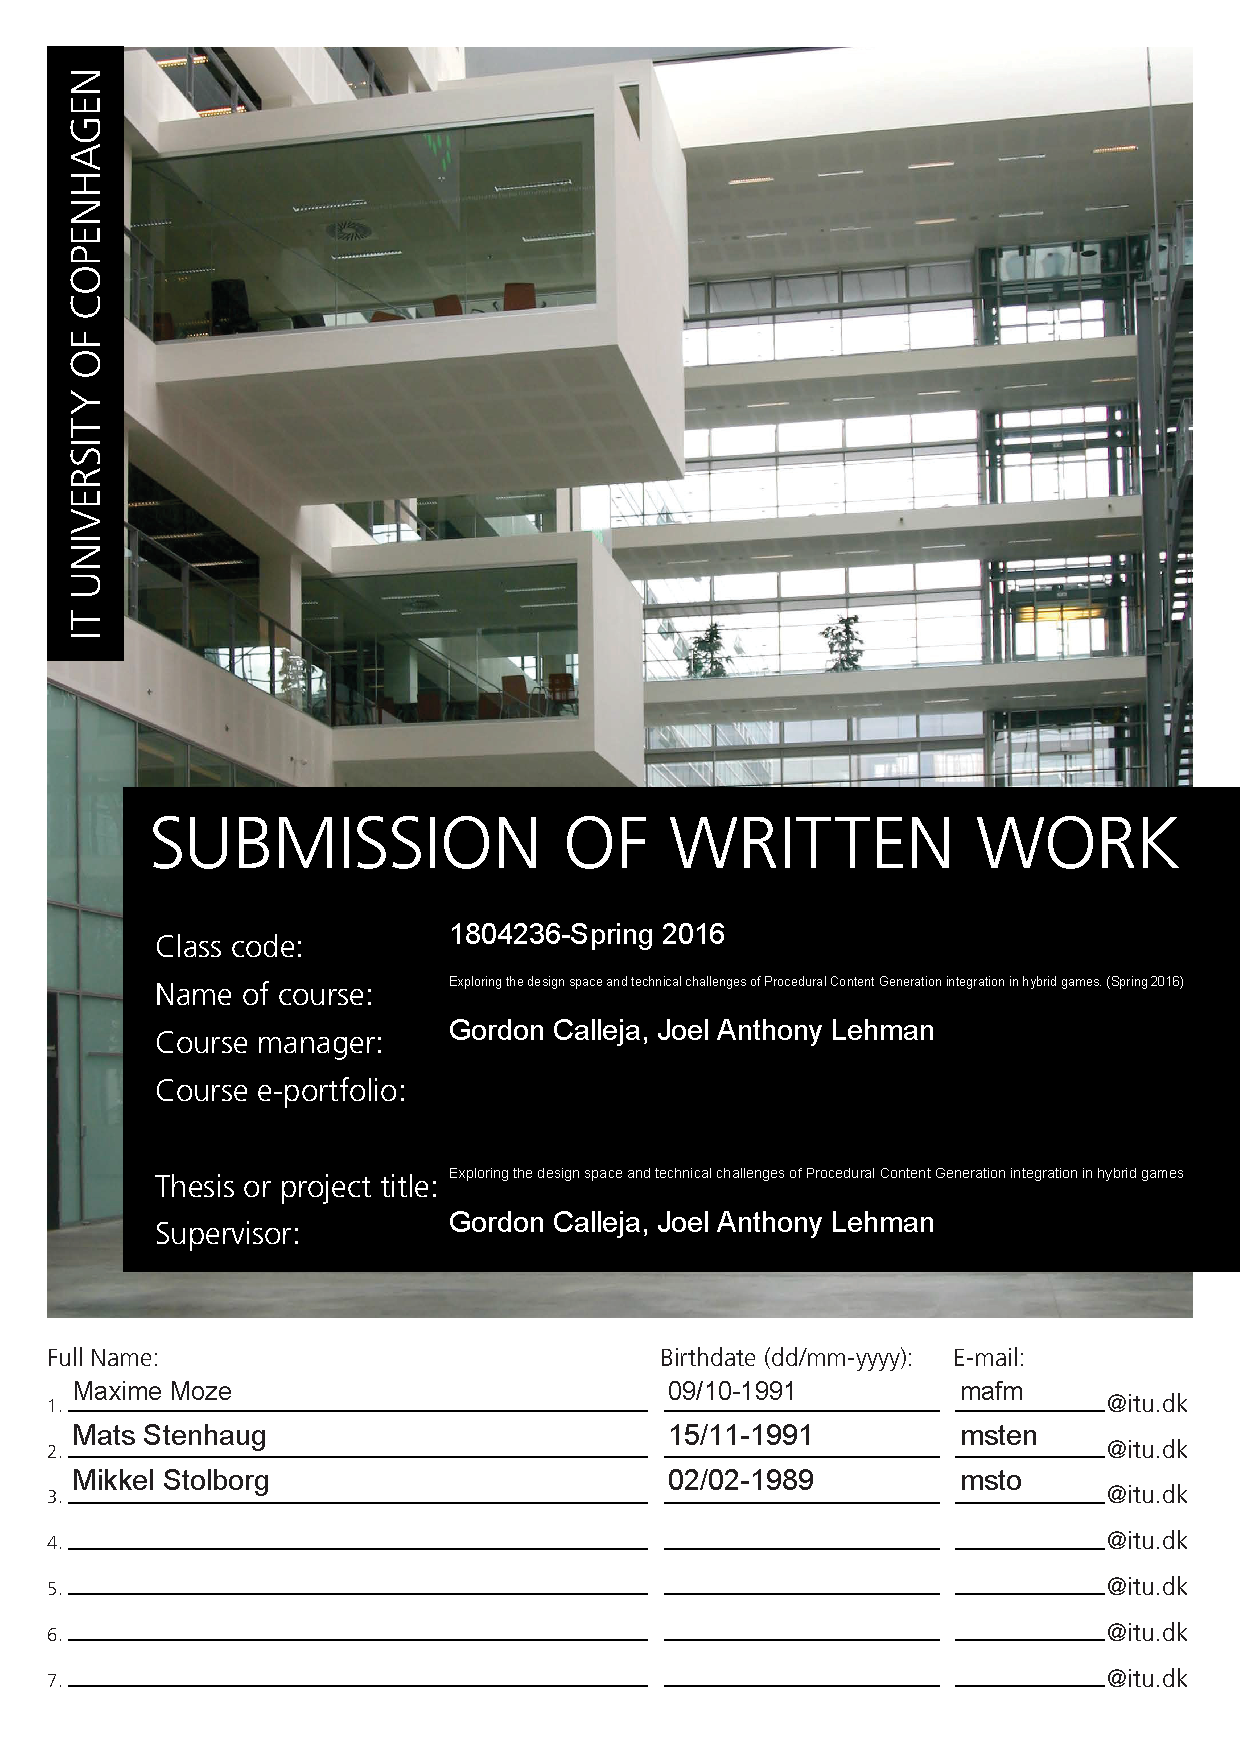
\includepdf[pages={1}]{MasterFrontPage.pdf}
\lstset{language=C}
 
\begin{titlepage}

\centering \parindent=0pt
\newcommand{\HRule}{\rule{\textwidth}{1mm}}
\vspace*{\stretch{1}} \HRule\\[1cm]\large\bfseries
Exploring the design space and technical challenges of Procedural Content Generation integration in hybrid games\\[0.7cm]
\large Masters Project\\[1cm]
\HRule\\[1cm]

%\begin{figure}[!ht]
	%\centering
%    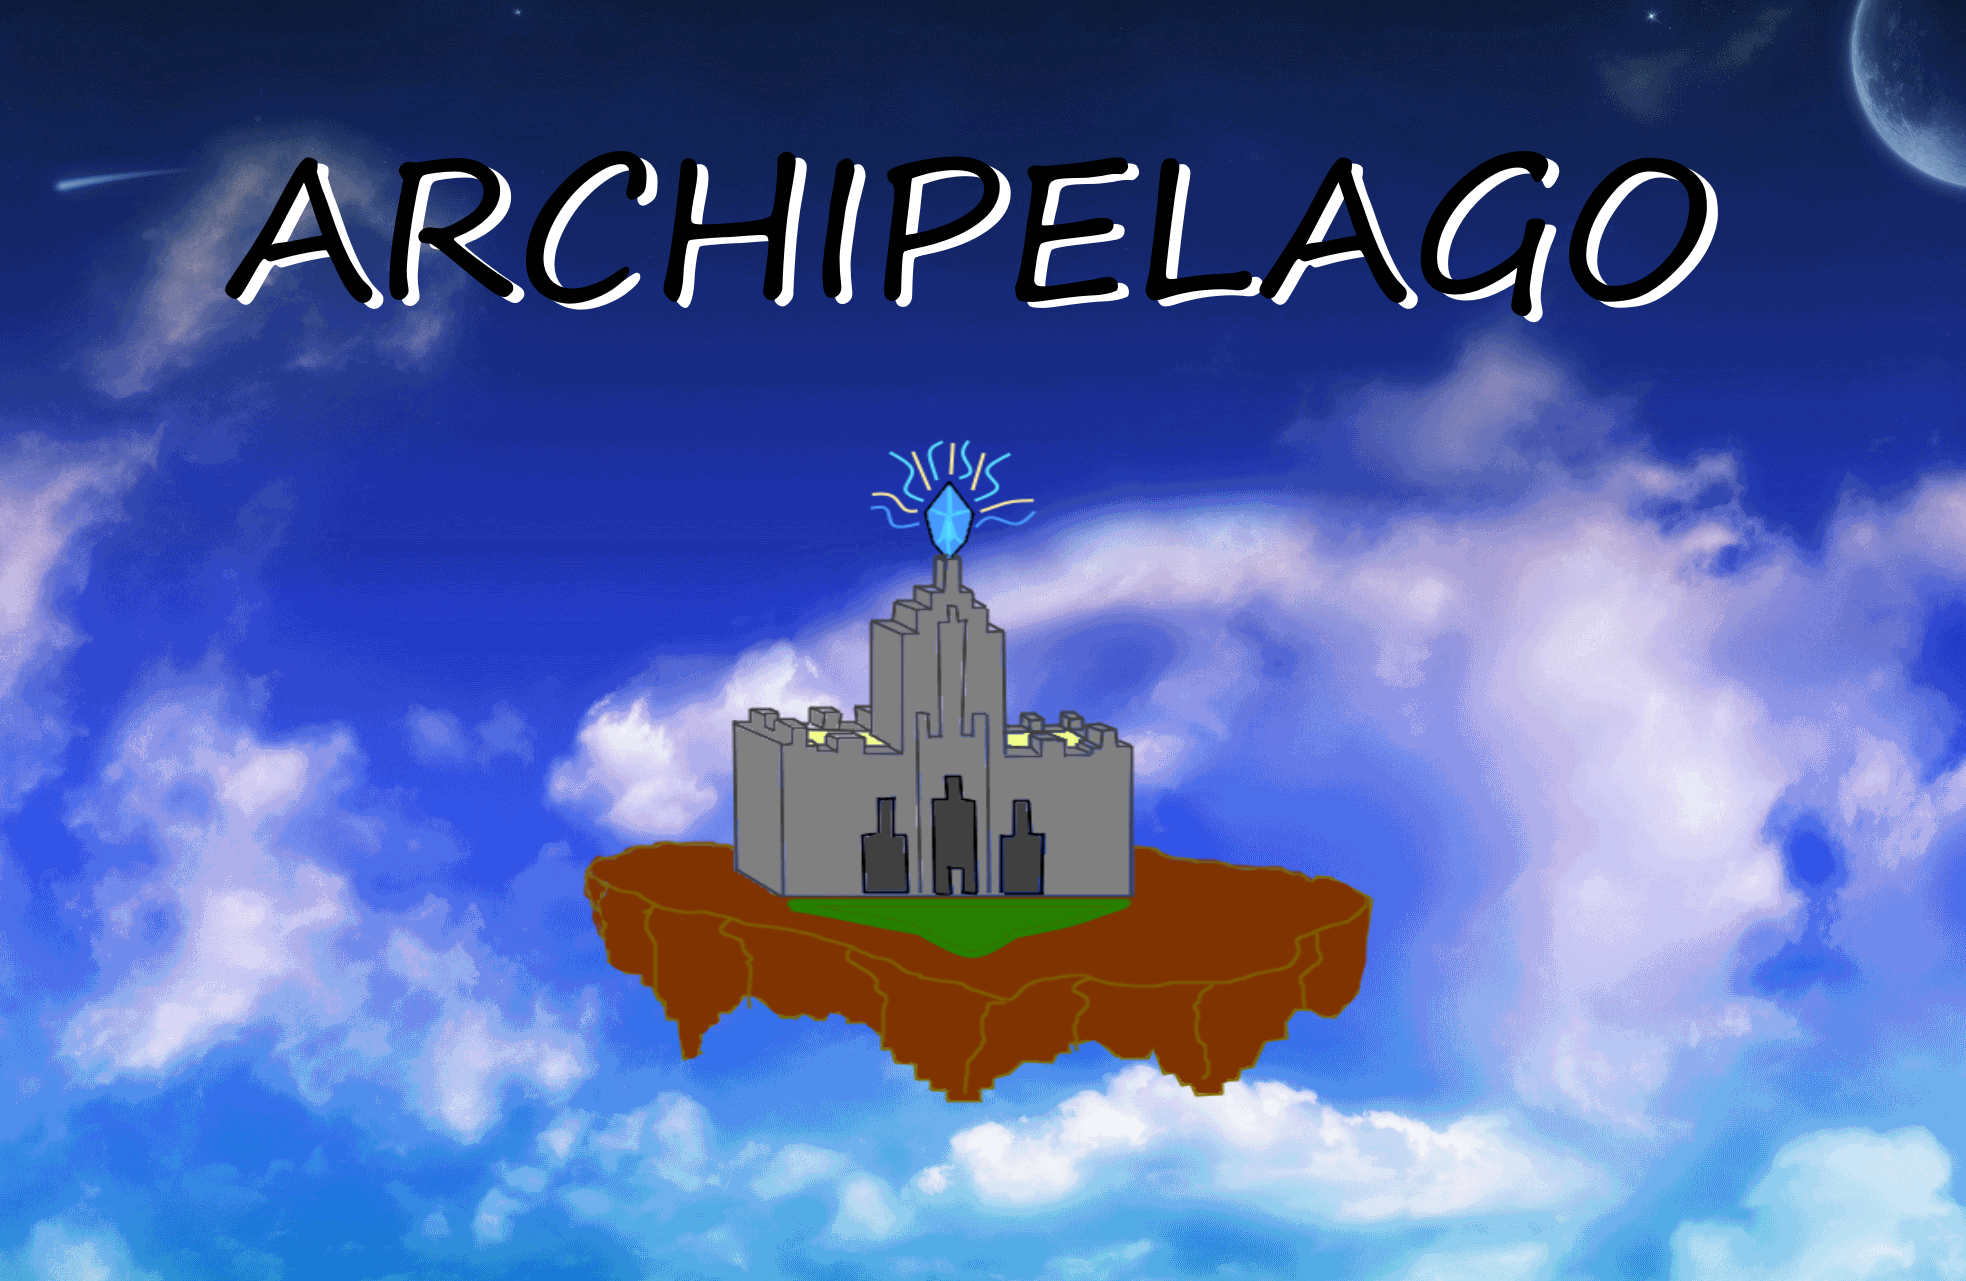
\includegraphics[width=1\textwidth]{Images/LOGO.png}
  %  \label{fig:frontPage}
%\end{figure}
\large by 
\\Mats Stenhaug (msten@itu.dk)
\\Maxime Moze (mafm@itu.dk)
\\Mikkel Stolborg (msto@itu.dk)
\vspace*{\stretch{2}} \normalsize
\begin{flushleft}
IT University of Copenhagen \\
\begin{figure}[!ht]

\includegraphics[width=0.2\textwidth]{Images/ITU_logo_ENG.jpg}
\label{fig:ituLogo}
\end{figure}
Supervisors\\
Gordon Calleja\\
Joel Anthony Lehman\\
\today \end{flushleft}
\end{titlepage}

\begin{abstract}
A new set of games are emerging as a combination of digital and analogue games. These hybrid games try to make use of digital components by the use of tablets, smartphones, and sometimes computers in collaboration with physical analogue tabletop games. 
This paper seeks to explore the possibilities of hybrid games through the design of one such game and implementing features to create play experiences which are not possible with only the analogue counterpart.
By using the application of Procedural Content Generation the hope is to generate content for the players which cannot be easily reproduced using traditional features in analogue board games. 
The game was designed over several iterations with feedback gathered from each prototype, both within the team and from external play tests. Analysing the data gathered before, during and after the creation of the game provided results on such digital implementation in tabletop games. 
The designed game produced special events using procedural content generation and basing them on the players action which they have performed during the game. The events are linked to the player actions such that they can see that the game remembers what they have already done.
The game manages to produce features which cannot be easily reproduced in a non digital context and which definitely would be cumbersome to manage in that situation. It also shows that there is potential in the use of digital components to solve complex calculations and that it can serve to add features which would be to intrusive in a non digital setting.
This paper discovers some of the beneficial aspects of Procedural Content Generation implementation within a hybrid game solution, and elaborates on different ways to utilize these discoveries along with other thought scenarios of implementation.

\end{abstract}
\pagebreak
\tableofcontents
\pagebreak
\listoffigures
\pagebreak
\section{Introduction}
Introduction to the ideas behind the project  ( Using PCG in a hybrid game)
Our problem statement ( Uncover a potential, adapt existing mechanics to a different media, explore a design space, create new mechanics / playful interactions…)
Why would you use PCG in a board game.
Most obvious challenges ahead
Uncovering less obvious problematics/challenges (thanks to the project)
Project scope and data gathering (Qualitative Methods)
The Roles of the group members.
Breaking the conventional way of board games
Thesis report layout. Short walkthrough of the report


PCG needs to be written with out the abbreviation in this section
An introduction to the name of our game



Some researchers try to think about analogue and digital games as a whole, and prefer talking about play as an activity instead of making a clear distinction between the two. This theory is crafted so that game studies are not distorted by the tendency of people to think about games in terms of mechanics or support (Stenros and Waern, 2010). In reality however, digital and analogue games are generally thought as two isolated categories of games.
\pagebreak
\section{Background}
This section will present the framework of this paper. First, existing game genres in which Archipelago takes inspiration from, as well as what have been identified as their key patterns will be defined. This definition process is important as a pre-emptive work to understand the bases on which the project was created. 

This will lead to a comprehensive definition of \textit{hybrid games}, and an identification of their core aspects. Furthermore, an analysis of early experiments showing a growing interest for hybrid games will be provided; this will help understanding the challenges implied by the development of hybrid games, as well as why the hybrid concept only reaches a wide audience now. This segment will be concluded by a play-through analysis of a hybrid game that is already on the market.

Because PCG was chosen to support the core mechanics of Archipelago, defining this programming concept is, and explaining how it is traditionally used in game design will also be a crucial aspect of this section. An overview of the technical definitions will be provided, followed by a description of the concepts that are important when designing with PCG. 

To complete this framework and before proceeding to the project in itself, important design theories will be presented. Those concepts are essential to boil down the critical elements identified by the definition and analysis processes, and to properly understand how hybrid games should be thought and conceived.
\subsection{Tabletop game play as a social activity}
It is commonly admitted that there are as many definitions of games as there are players. People working in the game industry, researchers, and players still disagree on which key elements should a taxonomy of games be based on. The french sociologist Roger Caillois (2001, p.3)\cite{book:mpg} explains the difficulty of establishing an all-inclusive game classification:
\begin{quotation}
The multitude and infinite variety of games at first causes one to despair of discovering a principle of classification capable of subsuming them under a small number of well-defined categories. Games also possess so many different characteristics that many approaches are possible.
\end{quotation} 
With this statement, one could argue that defining or classifying game genres is not relevant, as there will always be examples that do not fit the definition, which will then need to be extended and will therefore move away from its original meaning. This paper will certainly not bring a clear and universal definition of the game genres relevant to its topic, as definitions and taxonomies are necessarily affected by their research purpose. Nonetheless, basic definitions are needed to construct an understandable framework and provide tools that will help analysing the impact of the use of PCG in tabletop games, both on their design and creation and on the experience they enable.\subsubsection{Tabletop Games}
The definition of \textit{tabletop games} is the first one that must be refined in order to correctly comprehend the purpose of this paper. An example is needed as a reference in order to point out their key aspects. Game Designer Nat Levan (Oakleaf Games) gives his own definition of tabletop games. 
\begin{quotation}
The defining feature of a tabletop game is the need for components, not the need for a table. [...] [S]o perhaps saying that a tabletop game is a game with a structured placement of components establishes a better requirement (Levan, 2014)\cite{web:oak}.
\end{quotation}
\textit{Tabletop games} is a generic term used to refer to a broad variety of game genres that are played on a table or the like. They range from card games, board games, not forgetting miniature games or dice games. Although removing the need for a table from the definition seems rather counter-intuitive, this assumption is made to include other simple games using components. Nat Levan uses the example of the game of "guess what I'm holding in my hand"(Levan, 2014)\cite{web:oak} in order to justify his statement. Fully digital games are excluded from this range, although the line is sometimes thinner than one can imagine. The game \textit{Hearthstone: Heroes of Warcraft} (Blizzard Entertainment, 2014) for example, is a video game inspired from classical trading-card games\footnote{Card games in which players fight with decks of cards they collected and designed themselves.}. It uses the possibilities offered by digital devices to enhance a simulated tabletop experience: interactions with the surface on which the game is played, screaming voices to simulate an excited crowd watching the players or animations providing feedback when a card is played. The game goes far beyond what traditional trading-card games usually enable.

However, it seems that this approach is rather incomplete, because it overshadows the social aspect of tabletop games. It is understandable that tabletop games are not necessarily meant to gather people around a table to play. As an example, platforms allowing traditional tabletop games like \textit{Carcassone} (Wrede, 2000)\cite{game:carca}, \textit{Through the Ages: A Story of Civilization} (Chvátil, 2006)\cite{game:ages} or \textit{Race for the Galaxy}\ (Lehmann, 2007)\cite{game:race} and many others to be played online have made their appearance with the development of the internet. 
These games do not cease to be \textit{tabletop games} (even though the play experience is made different by changing the context in which they are played). This case is very particular though, as these online platforms solely propose an adaptation of already existing tabletop games, and do not use any advantages of digital devices to transform the games themselves, or create new ones. In that sense, it cannot be compared to a game that completely transforms the tabletop experience like \textit{Hearthstone: Heroes of Warcraft}.  However, this example really emphasizes a critical element defining tabletop games: these games need a space where the players can gather and participate to the play experience. In his work retracing the history of eurogames
\footnote{A particular type of tabletop game culture that has originated in Europe.}
, Stewart Woods (2012, p.212)\cite{book:euro} explains why the social aspect of tabletop games is a defining element:
\begin{quotation}
The play of tabletop games is a complex social activity.[...] [M]anagement of the immediate social setting in tabletop games adds a meta-level of understanding that cannot help but inform the process of play. The social context of the game can indeed shape play in a variety of ways, since players are always mindful of the social environment in which a game encounter takes place.
\end{quotation}
In consequence, the nature of tabletop games is what shapes the very particular play experience that they enable. Playing tabletop games means finding the right balance between being competitive and fair; and designing tabletop games also means supporting this shared experience and taking it into account. As long as they are made to be played by several players, tabletop games and their social dimension are inseparable (in the particular case of tabletop games meant to be played by only one player, this quality of tabletop games can be put aside).
\\\\
To complete the reflection, the next step of the process is to define what can be called \textit{components}, and why they have to be central in the case of tabletop games. Core components of tabletop games are generally thought as physical. They can be cards, tokens, pawns, dice or any object used as a core element in the game, which can therefore not be played without them. As is well known, tabletop games have generally evolved staying away from digital components. Exceptions exist though, and game makers have already experimented the use of technology to influence their design. The game \textit{Nightmare}\footnote{More generally known as \textit{Atmosfear} in the rest of the world, \textit{Nightmare} being the original title in the United States.} (Clements and Tanner, 1991)\cite{game:atmo} included a VHS tape showing "The Gatekeeper", who attributes rewards to the players, punishes them or gives them instructions at specific moments in the game, thus also acting as a timer. In that sense the VHS can be seen as a component in itself, like a deck of cards with a hourglass.

Components can then be defined as interactive elements without which the game cannot be played. The central dimension of components is clearly understandable, but it is important to notice that their physical property has been excluded from the definition.
\\\\
After these clarifications, it is now possible to come up with a definition of what tabletop games are. Tabletop games cannot be narrowed to the simple use of physical components, neither must they absolutely be played on a table; a more appropriate definition could be that tabletop games are games requiring the players to use their central components in a physical space in which player(s) gather, interact and participate to a social play experience. 
\subsubsection{Board Games}
\textit{Board games} are generally considered as a subcategory of tabletop games. Therefore, it can be acknowledged that the properties of board games derive from those of tabletop games. Oxford Dictionaries (2016)\cite{web:oxford} provide the following definition:
\begin{quotation}
"A game that involves the movement of counters or other objects round a board."
\end{quotation}
While this is a rather broad definition, it can still be used to present key aspects of board games. The terms "counters or other objects" refer to the core components that were previously mentioned as a key aspect of tabletop games. The new element here entering the definition being the game board, which is the surface on which the players move pieces, place cards or tiles in order to achieve the goal of the game. As it has been explained beforehand, this surface is not necessarily physical and can be then represented on a digital device like a screen. In a board game, the board is of course a key component. It is the center of the attention of players, and can serve several purposes.

The game board concentrates all the structural elements that the players should focus on in order to correctly play the game. It must support the play experience and also put limitations on the way the game is played. It that sense, it is as much an interface from which players extract the - more or less abstract - information they need, as it is an \textit{obstacle} forcing them to play according to the rules. In the game of \textit{Chess} for example, where planning and anticipation are the building blocks of the experience, those properties are clearly identifiable - though the board is not the most elaborate one. It limits the movement of the pieces within a square of 8 units of length, and a trained eye can easily identify valuable information (i.e. the movement possibilities), thanks to the tiled structure of the checker. 

One last property that can be identified, is that a board is rarely a core component in itself. During a game, the board only makes sense when it is accompanied by other core components like tokens or cards. Following the example of  \textit{Chess} again, the checker alone does not provide the necessary information in order to properly plan a strategy. It is only when the pieces are on the board that an experienced player can almost literally see the possible moves and anticipate the danger. This is only one example: game boards have different structures and purposes, and listing their properties here would not be relevant. But from those identified earlier, it becomes possible to give a definition of games using boards: \textit{board games} are tabletop games using a game board and its properties as a core component.
\subsubsection{Competition, collaboration and cooperation}
As Salen and Zimmerman explained (2003)\cite{book:rop}, "conflict" has clearly been identified as a defining element of games. Play enables a particular context in which conflict and the sense of achievement becomes the focus point of the experience. This particular context is what Salen and Zimmerman explain as a "magic circle" (Huizinga, 1938, cited in Salen and Zimmerman, 2003, pp. 94-95)\cite{book:rop}. It is a virtual space that is created by players in which all the participants agree to follow a certain set of rules that can be clearly identified (e.g. the rule book of a tabletop game) or unspoken (e.g. fair-play). While this is a metaphor that raises questions as much as it solves problems, it helps to understand why games can be thought as intrisically conflictual. Playing a game consists in a struggle towards the winning condition, which can of course take different forms. Trying to win is what provides a meaning to play in the first place, and all the potential experiences that appear while playing can be thought as a result of this race toward victory. Basing their reflection on this approach of game as system of conflicts, Salen and Zimmerman (2003, p.255)\cite{book:rop} explain the competitive dimension of games as follows:
\begin{quotation}
Our opinion is that all games are competitive. All games involve a conflict, whether that conflict occurs directly between players or whether players work together against the challenging activity presented by the game system.
\end{quotation}
This statement shows that competition must not be opposed to cooperation. While competition in games is traditionally  thought as a contest between players, it can also be considered as a struggle against the game. This is especially the case for single player games, in which the only obstacles that are placed on the player's way towards victory are set by the game itself. Competition is still present, and only its target changes. 

Yet, the authors do not make a distinction here between \textit{cooperating} and \textit{collaborating}. Though their respective approaches on the play experience can be expected to be similar, some researchers make the difference between cooperative and collaborative game play. Nash (2002, cited in Zagal and Rick, 2006, p.25)\cite{art:collab} argues that in cooperative games, the players have interests that are "neither completely opposed, nor completely coincident". In contrast, "in a collaborative game, all the participants work together as a team, sharing the pay-offs and outcomes; if a player wins or loses, everyone wins or loses"(Zagal and Rick, 2006, p.25)\cite{art:collab}. This differentiation between \textit{cooperation} and \textit{collaboration} makes a big difference in the play experience. As an example, \textit{Diplomacy} (Calhamer, 1959)\cite{game:diplo} encourages players to create alliances between them, and betray them when it is needed. On the other hand, in \textit{Forbidden desert} (Leacock, 2013)\cite{game:desert}, players have to manage the resources they individually possess and put their skills at the service of a team. 
This contrast is noticeable thanks to the interactions between the players. Collaboration involves more open discussions among the players and exclude the necessity to voluntarily hide information. Playing around this type of interactions outlines the tabletop game social play experience even more.
\subsection{Hybrid games}
\textit{Hybrid games} is an expression that has many different definitions, and the genre is still partially explored. Nonetheless, researchers have shown interest in this field and characteristics specific to hybrid games, derived from both tabletop and digital genres can be pointed out.
\subsubsection{Defining hybrid games}
There is not a universal understanding of what hybrid games are. Some people simply call \textit{hybrid games} games that are a combination, or hybridization, of two or more different genres of games. The interest of that definition is that it removes the analogue or digital aspect of games and simply focuses on the experience they provide. It needs to be refined though, because many games can be seen as a combination of genres, as game designers often build upon already existing game mechanics, trying to adapt them in another context. 

In this paper, \textit{hybrid games} are considered as a subcategory of tabletop games (and all their properties previously defined) using one or several digital components. They are based on the fact that players interact between each other by gathering around a space (like a board), and use the different components required to play the game in that space. The game structure has to support those interactions, thanks to its rules and mechanics. From that point of view, hybrid games are not that different from tabletop games - or even board games in some cases.

One criteria needs to be added though: as it has been already mentioned, the digital or analogue nature of the components does not change what defines tabletop or board games. Consequently, hybrid games must have another property. A game is much more than its components, game play mechanics or even its rules. De Boer and Lamers (2004, p.443)\cite{chap:aug} explain how the "possible electronic augmentation for board games" should be designed:

\begin{quotation}
[...] innovations should have a clear added value to the game concept and introduce new elements. Most importantly, the pleasure of playing a board game should be increased, while the existing physical elements of the game are preserved as much as possible. Summarizing, one could say that the added technology should fill holes in the game concept, that cannot be filled using traditional manners.
\end{quotation}

Therefore, only tabletop games including digital components in order to enable an experience that cannot exist without using the computing power of digital devices will be considered as \textit{hybrid games} in this paper. This aspect can of course take different forms depending on the game, like "randomly changing the board composition" or integrating "digital game rules" and "automatic error detection and prevention" (De Boer and Lamers, 2004, p.443)\cite{chap:aug}. Games that only use digital devices to simulate analogue game components (deck of cards or board for example) without providing any new feature are not considered hybrid games in this paper.

Another element must also be pointed out. Hybrid games are indeed a combination of patterns that can be found in digital games and in tabletop games. As such, their mechanic are in general not something new for an experience player of both digital and analogue games. However, the play experience delivered by this combination of patterns has to be original in its own way.
\subsubsection{A Hybrid Game Experiment: \textit{False Prophets}}
People have also started to refer to \textit{hybrid games} as games that try to close the gap between analogue and digital games. \textit{False Prophets} is an experimental game that explores "the space between board games and video games, leveraging the advantages of both" (Mandryk and Maranan, 2002)\cite{art:prophets}. 

\begin{figure}[h]
    \centering
    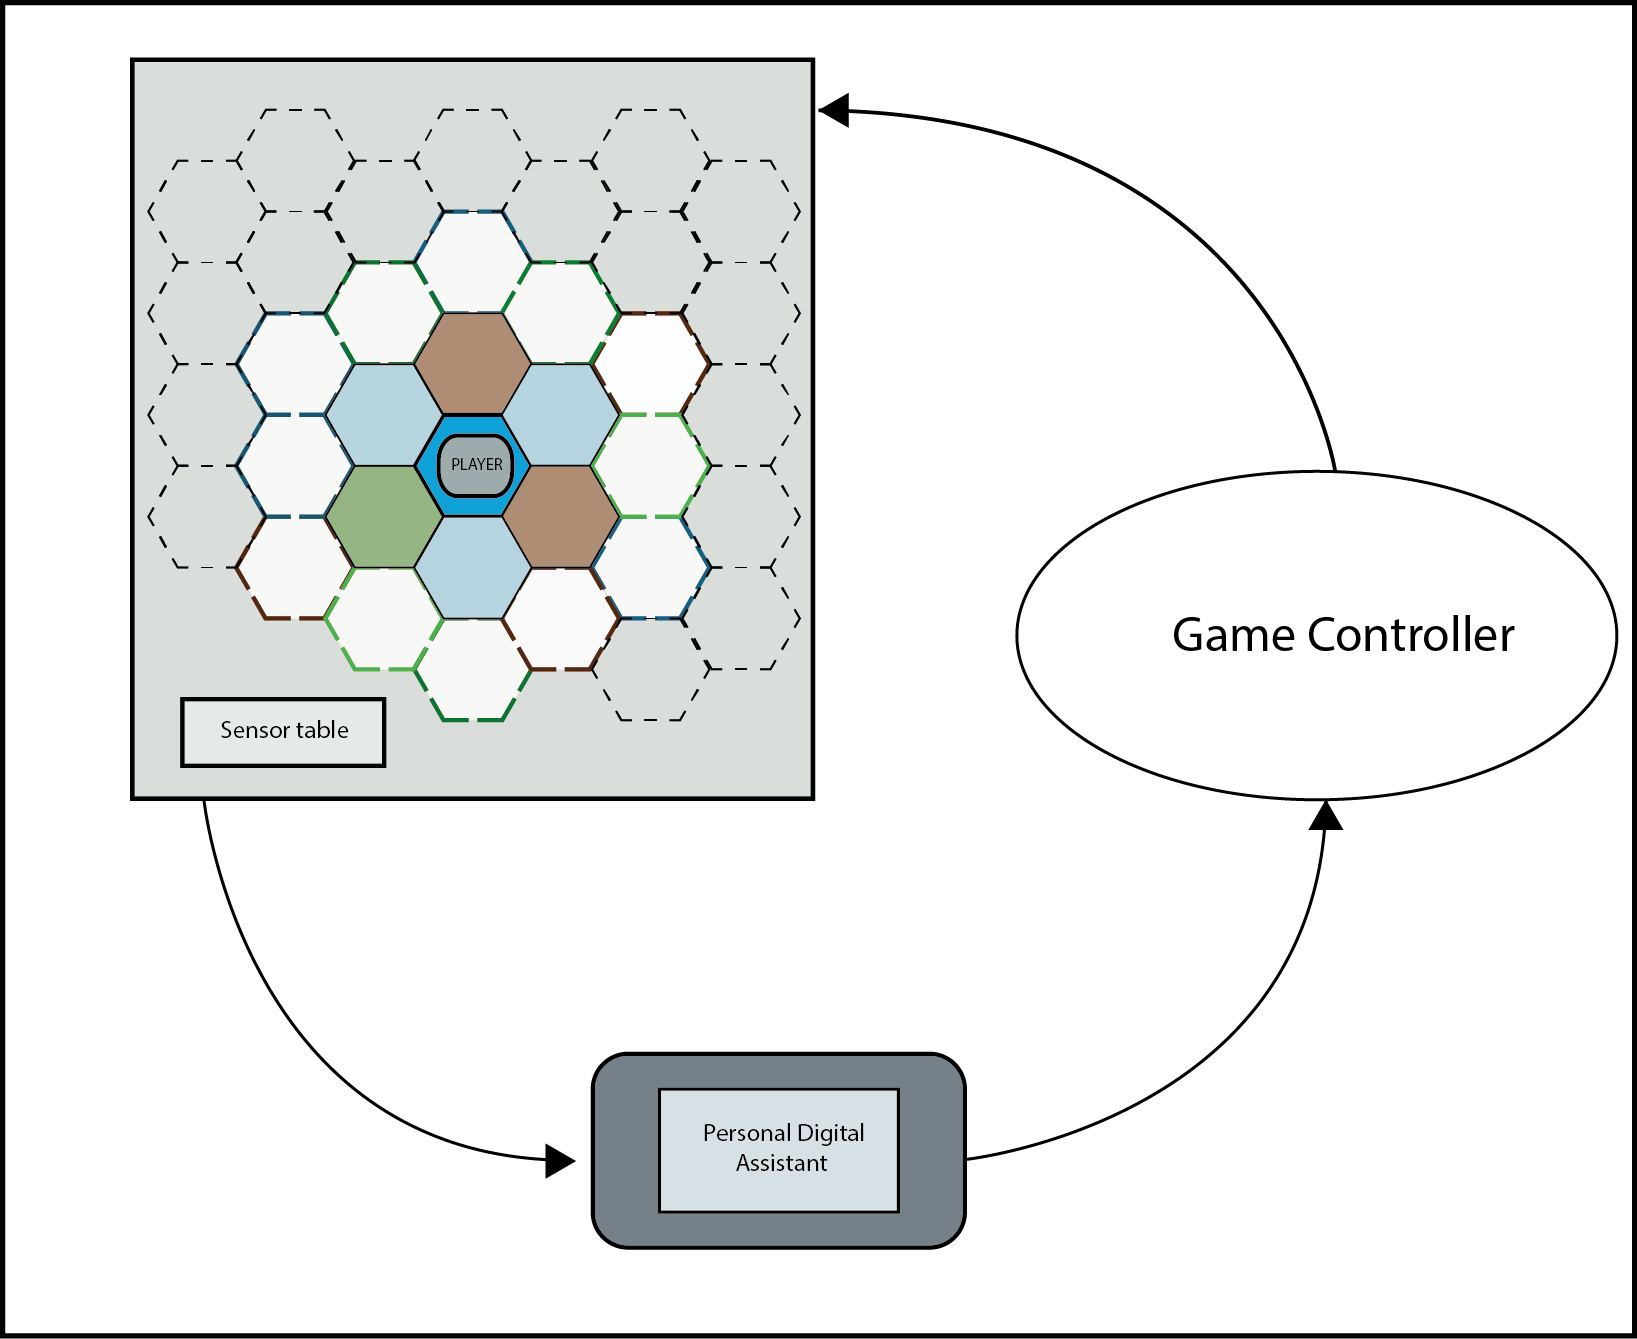
\includegraphics[scale=1]{Images/f_p_fig.png}
    \caption{A representation of \textit{False Prophet}'s set up. A hexagon tiled map is projected on a sensor interface. Only the tiles that are close enough to the players are displayed. The colours represent the different types of terrain they are. The players also have a handheld computer used to display some relevant information. The devices are linked to a game controller that handles the computation required to display the map, or communicate information to the players.}
    \label{fig:falseprophet}
\end{figure}

This experiment was a technical challenge more than a game design experiment. Mandryk and Maranan created a tabletop display using sensors in order to recreate an interface. A tiled map made of 20x30 hexagons is projected on a surface containing infra-red sensors, which can detect the position of the tokens in the displayed tiles. Originally, the hexagon tiles are hidden, except for the one on which the player tokens are placed. It is only when the game's computer detects players moving their tokens that the closest tiles get revealed. The map is linked to a game software that takes care of updating the map, and detect the game pieces. The handheld computers are used to perform actions that cannot be communicated through the game pieces. For example, logic puzzles have to be solved during the game: this is made thanks to the handheld computers, which are also linked to the game controller (see figure\ref{fig:falseprophet}). 

The players are separated in two teams, but the players do not know their team member. The goal of the game is to discover who belongs to which team. To get information about the other players and guess in which team they are, the players move their tokens close to each others. The closer two pieces are, the more detailed the information is. 

The designers were aware of the need to encourage direct communication between the players, and made rules that support such interactions. For instance, direct communication between the different players is not supported by the game system (while this would have been possible thanks to the handheld computers). To exchange clues, the players have to do so verbally, thus forcing them to interact between each other. 

The interest of this experiment is that it tries to exploit the assets of both game boards and computers. First, it uses the context of having an interface around which players can gather and encourages direct communication thanks to certain rules, thus respecting the social nature of tabletop game. Mandryk and Maranan clearly outline their understanding of tabletop games even before entering in the details of the conception of \textit{False Prophets}. Their game is flexible enough so that players can bend the rules if they want to, and they primarily use a board to encourage the interactions between the players, instead of designing it only to transfer information between the player and the game (2002)\cite{art:prophets}.

Second, computation can be used to do complex calculation that would be impossible to do for humans while playing the game. In this case, the manifestation of that is the map that gets revealed dynamically.  While fully analogue games  that possess a similar mechanic, like \textit{Zombies!!!} (T. Breitenstein and K. Breitenstein, 2001)\cite{game:zombies} already exist, the sensor interface could allow many possibilities for game mechanics. This is a typical example of exploiting the digital device, allowing to enable a kind of play experience that is totally new to tabletop games. As a future work, the creators of False Prophets mentioned having "playing pieces that store data, interpret contextual information, and travel continually with the players" The other digital device (the handheld computer) however seems to be thought as a support for all the actions that "cannot naturally be communicated through the game pieces"(2002)\cite{art:prophets}.

By combining the advantages of computation (that is generally used in digital games), and those of board games (allowing a strong interaction between the players), \textit{False Prophets} represents an interesting approach to the genre of hybrid games. It also proves that hybrid games deserve to be thoroughly studied, and that a huge amount of variety can be brought to the world of tabletop games by exploiting digital components.
\subsubsection{\textit{STARS}, the hybrid game platform}
During the Ubicomp '03 conference on ubiquitous computing environment\footnote{"A proposed development of computing in which computers are sufficiently small and inexpensive to be embedded frequently in everyday objects."(Oxford Dictionaries, 2016)}, Magerkurth, Stenzel \& Prante (2003) showed \textit{STARS} \cite{art:stars}, another example of the integration of digital devices in the traditional way of playing tabletop games, though even more complex than \textit{False Prophets}. This project was elaborated as an attempt to show the many possibles interactions between different devices "by realizing computer augmented tabletop games [...] within a smart Roomware® environment" (2003)\cite{art:stars}. In other words, different hybrid games, or adaptations of already existing tabletop games could be played using this platform.
\begin{figure}[h]
    \centering
    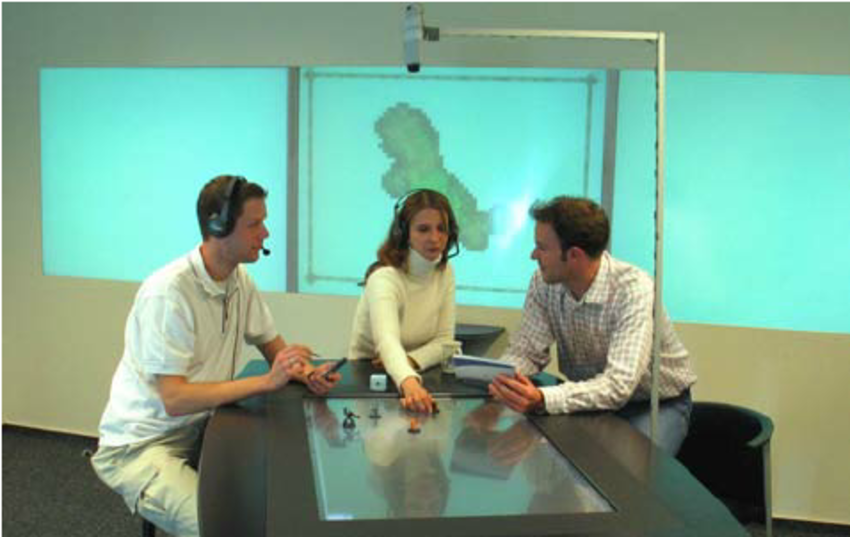
\includegraphics[scale=0.4]{Images/roomware.png}
    \caption{The Roomware® environment used to create \textit{STARS}. The camera detects the position of the different game pieces on the interactive table and. The wall displays are used for public informations and the Personal Digital Assistants for personal, non-shared information. Audio devices are used for communication.}
    \label{fig:roomware}
\end{figure}
The \textit{STARS} platform features an interactive touch-sensitive screen, which displays the content of the game board as well as it manages the interactive playing pieces. A camera is situated over the table and tracks the position of other playing pieces. \textit{STARS} also features a wall display and other digital components like a small Personal Digital Assistant (used by the players to secretly communicate and store personal information related to the game), and audio devices. All the devices are interconnected and managed by a game software (see figure \ref{fig:roomware}). 

Although this experiment looks similar to False Prophets, this multi-device approach is the interest of the project. By exploiting the possibilities offered by the different component of the computing environment, the creators hoped to "go beyond traditional tabletop games, but at the same time preserve the human centered interaction dynamics which makes playing board games a joyful group experience"(2003)\cite{art:stars}. The social dimension of the tabletop game play experience has been used here to prove the efficiency of an interconnected digital environment. The benefits of using such interactive platform has been explained as follows:
\begin{quotation}
Regardless of the number of players involved, playing computer games is still being perceived as a mostly isolated activity. This is due to the interaction being technology centered.[...]The richness of human-to-human interaction
involving eye contact, mimics, and gestures is far from being captured in the purely virtual gameplay of computer games.[...]To further augment the social experience of computer games and facilitate a strong emotional involvement among the players, direct face-to-face interaction should be enabled and new interfaces between the players and the virtual domain must be introduced (Magerkurth, Engelke \& Memisoglu, 2004)\cite{art:stars2}.
\end{quotation}
It could be argued that the statement simplifies too much the interactions between players in digital games, but the approach shows an understanding of the particular relationship between players in a tabletop game. The platform encourages such \textit{computer assisted} interactions, and also opens to the possibility of creating other tabletop games using digital devices as core components, thus enabling new play experiences. Three different game adaptations to the \textit{STARS} platform are described (2004)\cite{art:stars2}.
\begin{itemize}
\item\textit{KnightMage} is a hybrid game that was developed for the \textit{STARS} platform. Its rules are based on classical Hack'n'Slash games\footnote{Term that referred to a type of gameplay in "pen and paper Role Playing Games" such as \textit{Dungeons and Dragons} (Gigax and Arneson, 1974\cite{game:dnd}), before becoming the common denomination of a computer game genre}, in which the players go through dungeons, kill enemies and gather equipment to improve their character and progress through the game. According to its creators, \textit{KnightMage} was designed to "combine the strong social situations of traditional tabletop role-playing games with typical benefits found in computer adaptations of role-playing games" (2004)\cite{art:stars2}. The typical Hack'n'Slash mix of cooperative (fighting the monsters) and competitive (gathering the best loot) gameplay, combined with the physical interactions with the game core components is what enables a new hybrid game play experience based on design patterns extracted from both digital and tabletop game genres.
\item\textit{Candyland}\footnote{Not to be confused with the board game \textit{Candy Land}(Abbott, 1949)\cite{{game:candy}}} was a hybrid game designed for children. The game takes place in a small village that the players can build by placing the components on the tactile table. The game software creates an interactive story based on the children actions. This shows another type of hybrid game model.
\item\textit{Monopoly Adaptation} is based on the classical \textit{Monopoly} (Darrow, 1935)\cite{game:mono}. This experiment is an attempt to show the potential of adapting traditional board games to the \textit{STARS} platform. The adaptation removes the most tedious actions like shuffling cards, managing all the bank notes, and components on the board. To create a new experience, new mechanics made possible thanks to the use of a digital device have been added to the original game. For example, the players can now secretly transfer money to another player in order to form alliances.
\end{itemize}
With a platform like STARS, it could  be argued that the quantity of available information (on the board, the wall display and the Personal Digital Assistant) might get in the way of play by making it too complex. But this invention is interesting in its approach of hybrid board games: it uses the potential of digital devices as core components, enabling new hybrid play experiences that would hardly be possible otherwise.
\subsection{The Hybrid Games market}
The \textit{False Prophets} and \textit{STARS} experiments are early attempts to introduce digital components into tabletop games. However, the complexity of such devices made it very difficult to turn them into a commercially viable product. 
\subsubsection{Development problematics}
As a conclusion of their research, De Boer and Lamers explain the difficulty of developing hybrid games:
\begin{quotation}
The electronic augmentation of board games is still in its infancy. World leading board game manufacturers, although sceptic, are willing to invest resources in the development of such games. Important obstacles are the costs of development and production and the need for game designers to accumulate knowledge on modern technology (De Boer and Lamers, 2004, p.444)\cite{chap:aug}.
\end{quotation}
It is true that hybrid games involve a new type of parallel development between the physical part of the game and the device(s) supporting it and making it hybrid. It involves a transformation of game studios, as well as new possibilities to explore for game designers. An explanation could be that the gap between two industries with few interconnections. This can be noticed in game conventions, where the digital games attract a bigger audience every year while tabletop games are relegated to a small isolated room. This does not mean that playing tabletop games and playing digital games are two incompatible activities; but there is a lack of recognition between the two whereas they are fundamentally based on the same activity: play. This leads to the problem of target audience.

Target audience is an important concept in game design. Not only is it important to know for who the game is made in order to create a product that can be sold on the market, it is also the bases of many design decisions. The approach of hybrid games illustrated by the two experiments shows the lack of a common ground on which to base the games. Saffer describes the thoughts behind a user-centered design with one simple sentence: "users know best" (Saffer, 2010, p.33) \cite{book:id}. This idea could explain why the implementation of digital devices in tabletop games was not popular.  An unclear definition of the target audience, due to the rapidly evolving habits of players regarding digital devices made it hard for designer to focus on a technology to build design decisions.

Primarily, one could think that the main target audience of hybrid games lies in a blurry zone between computer games players and tabletop games players. Tabletop game players are used and attached to the \textit{ritual} (this term can be emphasized because this is exactly how some tabletop game players perceive it) of preparing the board, manipulate physical game components and trying to understand what is the game about before even reading the rules; it is probably the opposite for people playing digital games who are used to learn how a game works, either with a clear step-by-step tutorial, or thanks to in-game (sometimes hidden) clues placed by the designers to understand the game mechanics. Therefore, there is already a problem when designing a hybrid game for the two groups at the same time and the target audience becomes more complex than it seems, and using devices that all the potential players never saw or used before probably did not help when showing the concept to game publishers. This problem was solved by the rapidly increasing popularity of smartphones and tablets.
\subsubsection{A growing interest}
The recent and rapid development and the adoption by a large audience of easily connected devices has provided to developers a natural and heavily supported material on which hybrid game mechanics could be based. Many possibilities are already known by the designers (who probably already possess the devices for their own personal use) and the development of a smartphone or tablet application does not require a very specific programming knowledge (like it was the case for an environment like Roomware®). For that reason, hybrid games have recently started to develop on the market, and could well be a natural evolution for tabletop games if the audience follows.

It has been previously explained in this paper that simple adaptations are not the focus of this paper (though interesting in the way they change the traditional tabletop experience). One thing needs to be mentioned though: those adaptations seem to be what really started the growing interest for digitally enhanced tabletop games. Some games like \textit{Ticket To Ride} (Moon, 2004)\cite{game:ticket} or \textit{Small World} (Keyaerts, 2009)\cite{game:tw}, have seen an surprising increase in the sales of their physical versions, when the digital versions were published on smartphones and tablets for a much lower price(McElroy, 2013)\cite{web:poly}. This proves that the so-called separation between the analogue game target audience and the one of digital games is not as big as expected.

\textit{Zombicide} (Guiton, Lullien and Raoult, 2012) \cite{game:zombi}, seems to be one of the first innovative examples to implement digital components to enhance the tabletop experience. Designers rapidly saw the interest of the experience:
\begin{quotation}
The app maximizes gameplay by virtualizing the mundane aspects, like dice rolls and card shuffles, and allows players to focus their energy on strategizing their next move. You can play the game without the app, but doing so is like wandering into a zombie-infected street without a shotgun or machete (Flaherty, 2012)\cite{web:wired}.
\end{quotation}
The fact that \textit{Zombicide} can be played without the application makes the game fall out of the definition of \textit{hybrid games} (the digital device is not a core component in that case). However, the success proved the commercial potential of such design, and others followed in its steps.

\begin{figure}[h]
    \centering
    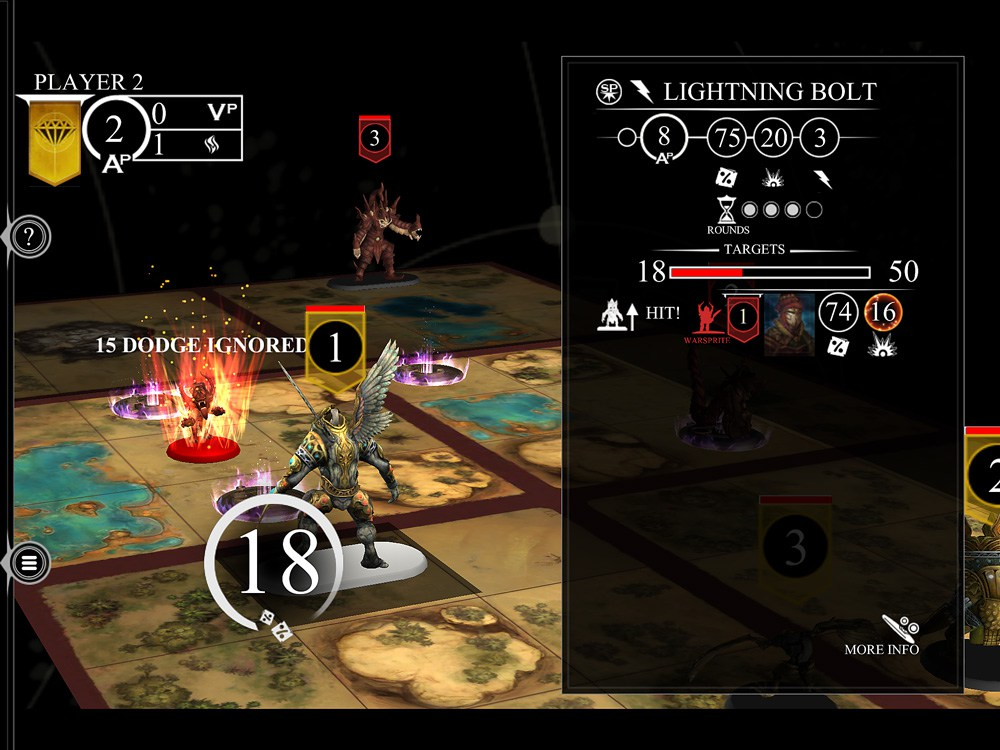
\includegraphics[scale=0.2]{Images/golem_app.jpg}
    \caption{The resolution of the fights in \textit{Golem Arcana} as they are displayed on the app}
    \label{fig:Golem}
\end{figure}

\textit{Golem Arcana} (Harebrained Schemes, 2014)\cite{game:golem} is often cited as one of the most innovative recent example of tabletop game experience enhancement through the implementation of a digital device (Banks, 2014)\cite{web:golem}. It is a battle between to players, based on miniatures that are moved on the board. This case is particular though: the game uses a Bluetooth stylus to recognize the pieces that are used on the board, in order to transmit the informations to the application. When a battle between two golems occurs, the players can choose between rolling dice and calculate the damages, or let the application do all the maths. The mechanic itself is not dependent on the digital device, but the experience is greatly improved by the fun of  "tapping your target with the stylus and then turning to your phone or tablet and watching as hit points disintegrate from your target" (Banks, 2014)\cite{web:golem} (see figure \ref{fig:Golem}). However, the whole game cannot be played without digital devices: the application is used to chose between different scenarii, which declares how the board must be set up at the beginning of a game. Moreover, the game rules are explained through the devices, which is cited as an advantage that makes the game very accessible.

All these examples prove the development of the hybrid game genre. The games have evolved from simple adaptations of existing games that have attracted the attention of a wider audience, to games that use the digital devices to enable a new experience. 
\subsubsection{Playing a Hybrid Game - \textit{XCOM: The Board Game}}
This overview of the hybrid game market will be concluded by a play-through analysis of a hybrid game as defined in this paper: a board game that uses a digital core component to enable a new kind of play experience. This has been done while developing Archipelago, in order to understand the impact of such an implementation.

For the majority of players, X-COM (sometimes written "XCOM") is a series of video games which first episode was \textit{UFO: Enemy Unknown}\cite{game:xcom} (Microprose, 1994)\footnote{Also known as \textit{X-COM: UFO Defense} in its north-American version.}. The series has many episodes and spin-off, and also a tabletop game plainly called \textit{XCOM: The Board Game} (Lang, 2015)\cite{game:xcomtbg}.
\begin{figure}[h]
    \centering
    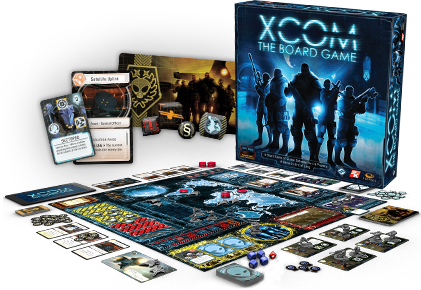
\includegraphics[scale=0.5]{Images/xc01_layout.png}
    \caption{The content of \textit{XCOM: The Board Game}}
    \label{fig:XCOMBG}
\end{figure}
What makes this game interesting for the purpose of this paper is its use of a digital component: an application which has to be downloaded on a digital device (smartphone, tablet or computer) (see figure \ref{fig:XCOMBG}) or opened in a web browser. The game simply cannot be played without this application, since it displays instructions that the players have to follow. On a certain extent, it cannot even be learnt without it: in the box, only a very short leaflet explains how to set up the game and where to find the application. The rules book is not included in the package - which can be disturbing for some players. Instead, all the rules are explained during the - optional - tutorial phase explaining the flow of the game, step by step. 

The game is described as a one to four players cooperative game. However, since the players share the same interest and goal, the game actually falls the definition of collaborative games that has been previously explained in this paper. Therefore, this is how the game is going to be referred as from now on.

In \textit{XCOM: The Board Game}, the players are part of the \textit{X-COM}, a paramilitary organization that defends the Earth against an alien invasion, after all the regular armies have failed to do so. The game's board is a representation of a world map, with other boxes used for the different game mechanics.

Fist of all, there are several levels of difficulty available. It must be selected prior to starting the game. The level of difficulty affects in various ways the instructions given by the application integrated in the game.

\begin{figure}[h]
    \centering
    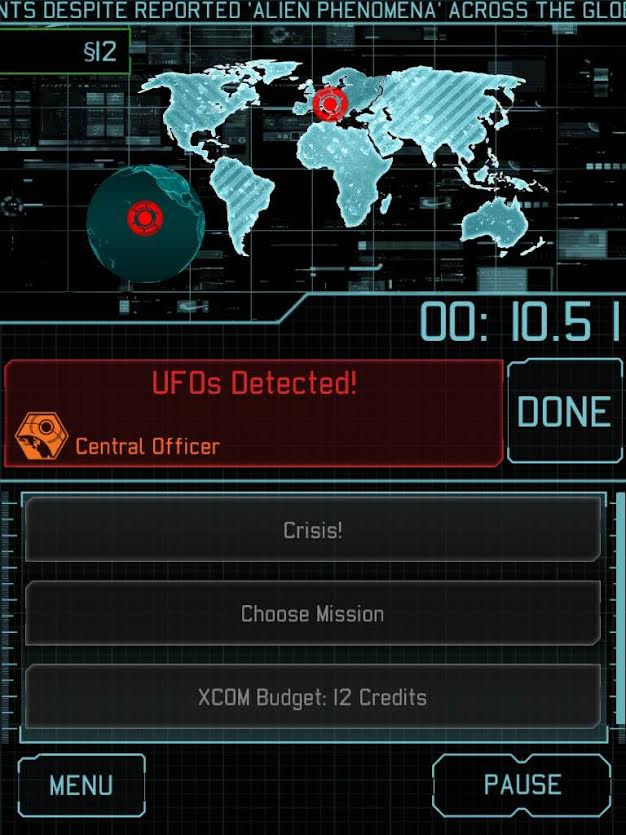
\includegraphics[scale=0.3]{Images/xcom_boardgame_app.jpg}
    \caption{Instructions displayed by the app during the timed phase}
    \label{fig:XCOMAPP}
\end{figure}


One round is divided in two phases: the Timed Phase and the Resolution Phase. The companion application tells the players the order of the different tasks that constitute one phase, as well as how much time is available to finish it - knowing that the order of the tasks changes over the rounds (see figure \ref{fig:XCOMBG}). The tasks are a preparation for the resolution phase: the players discuss to allocate resources in the best possible way, assign soldiers to defend the \textit{X-COM} base, or prepare to repel the next alien attack. The players also have missions to solve, which are a good way to get more resources. There is also a final mission that the players have to complete in order to finish the game. As its name suggests, the players have limited time to perform the tasks during the Timed Phase, but there is a Pause button in case the players need more time to think about the best way to perform the tasks. In the normal and higher difficulty modes, the time during which the game can be paused is limited but is renewed at the beginning of each round.

During the Resolution Phase, the players solve the tasks they have prepared during the Timed Phase. This often takes the form of dice rolls. The tasks to solve are different depending on the player's role. At the end of the Resolution Phase, the player responsible for managing the digital device is asked to enter a few information about the round (i.e. what is the current panic level of panic for each continent and if a mission as been successful or not). These inputs are necessary for the application to generate the locations where the aliens will spawn during the next turn. Four roles must be split between the players (they can have more than one role in case of a game with less than four players):
\begin{itemize}
\item The Central Officer is the only player that has to use the digital device, she has to relay the instructions that are displayed on the application to the other players. Also, the Central Officer is responsible for placing the alien tokens at the right on the game's board when instructed by the application. She can also decide when to use the pause button to give more time to her team.
\item The Chief Scientist researches alien technologies when instructed by the Central Officer (relaying the instructions given by the application), which are bonuses that help the other players (or the Chief Scientist herself) performing their tasks.
\item The Squad Leader controls the ground soldiers. This is done to defend the base when it is attacked, and when trying to solve one of the missions. The dead aliens are used as a resource by the Chief Scientist to develop new technologies.
\item Performing tasks cost money. The Commander is the player responsible for the budget, and thus manages an overall strategy. She also deals with the UFO that are spawned all over the world. If one of the continent is not defended correctly, its panic level increases, and it becomes even harder to defend. When two continents have reached the maximum panic level, the game is lost.
\end{itemize}
\textit{XCOM: The Board Game} definitely shows how the use of a digital device can enable interesting playful experiences. The fact that the Timed Phase is indeed limited in time is not an absolutely new feature in itself. But once the available time to perform a task is up, the next task starts directly and the players have to abandon what they were doing and move on in order to keep up with the application. Because of this, playing as the Chief Officer nicely recreates a feeling of being the one without whom the team would be overwhelmed by the flow of the game. The instructions coming from that player have then to be clear, and quick. The combination of the time limit with the random order in which the tasks have to be performed creates a feeling of constant emergency during the Timed Phase. Succeeding in performing all the tasks in due time, feels relieving and rewarding, as the team coordination is working correctly. Players learn how to rest on their team members while doing their best not to fail. This model of team dynamic would hardly be possible to recreate without the use of the digital device, because of the number of game pieces that would be required to simulate it. Here, the device simply uses a combination of some of its basic functions, and some player inputs. The simplicity enables an experience that would be impossible without a digital component. Therefore, the game deserves its status of \textit{hybrid game}.

Aside from what it brings to the play experience, the way the application is used to teach the game is also interesting. Traditional rulebooks usually follow a step-by-step process as well. But the application encourages the players to perform all the actions one by one, while the explanations are displayed. This make the rule learning phase very similar to strategy video game tutorials, where the players are encouraged to use a unit to learn its potential. This combined with the collaborative game play, where smaller tasks are divided between players makes it very easy to learn how the game works. It is not surprising that the game can then be won without even knowing exactly what the other players had to do.

The device is normally not too intrusive in the game, as reading the instructions fast and clearly is part of the experience. The only aspect that interferes with the experience being the moment when the player holding the device has to enter some inputs, so that the information about what happened during the turn can be filled to the device. Nonetheless - because it is an uncommon component to use in a tabletop game - not having to do anything with the device itself can feel a bit frustrating for some players. A last detail is also worth noticing when analysing a hybrid game like this: the game flow can be completely annihilated if the device runs out of battery - which can be very frustrating when playing a tabletop game. 
\subsection{Procedural Content Generation}
To design Archipelago, it has been decided to use PCG in order to explore hybrid game mechanics. To understand what this implies in terms of technology, design and development, a description of the technical concept, as well as its common uses in game design will be provided in the following paragraphs.
\subsubsection{A content creation method}
\begin{quotation}
"Procedural content generation (PCG) refers to the algorithmic creation of content. It allows content to be generated automatically, and can therefore greatly reduce the increasing workload of artists." (Rolan van der Linden, et al., Procedural generation of dungeons, March 2014). \cite{art:pcg}
\end{quotation}
This quote tells us that PCG does not really have anything to do with the playing of the game it self, rather the contents within it, hence the name procedural \textit{content} generation. 
However, it is not always as simple as that. The line between when the content is being generated by the user and what is generated through assisting the user is fuzzy.
As an example from \textit{What is Procedural Content Generation? Mario on the borderline}\cite{art:whatpcg}, the players interaction with the game \textit{Sim City}, generates more content indirectly based on the interactions. This kind of can be described as Computer Assisted Design. As explained however, there is a very thin line between when the game ends and the algorithms start. 

The place where the line get blurry is when the algorithms generate content based on human input. The reason it is a grey area is because it enters the region of computer assisted design(CAD)\cite{book:cad}.
It is becoming more accepted within larger companies, as a way to lighten workload of other artists, and its uses range between various fields.
To build on what R. van der Linden, et al. say in their paper, about reducing workloads, PCG is a great tool to create templates for content, based on data from designer, artists, etc. PCG can also be used as a tool for aiding in creating content.  
The general idea behind this is that a tool generates some content or usable structure, which it then exposes to a designer. The designer can tweak parameters and sometimes directly interact with the generated content. This way a designer might be presented with a basic structure of a tree, and then have the ability to add branches and leaves, which are in turn generated by the tool. 
The work of the artist is aided by the computer, giving the artist more time to work out the details. Computer generates templates and a base, then it is up to the artist to look over the content and see whether it is pleasing enough, fun enough, and/or acceptable in the final form. The final idea behind this is that it is in the minds of humans that creativity lies. 

PCG allows to generate more content without putting more effort into the manual work in order to populate one's virtual world. With pcg you can design the template and rules you want in order to generate a wide range of items for your game, without having to design each individual item or use copies of the same few items. An example is the application is the tool called \textit{SpeedTree}. This application allows for the generation of different tree which can be used in the environment without having the feel of a copy paste environment. In this PCG allows the designers to focus on creating interesting game play and environments and leaves the details of the individual structures to the pcg tool. 

PCG can also be used to generate a larger play space, by allowing for near infinite variations and/or generations, the replay experience is varied enough to allow for greater replayability in total. Games such as \textit{Age of Empires} and \textit{Civilization} are well known for their map generation, creating playable and enjoyable maps, each different from the last.


Other aspects within the PCG world, which is becoming more and more accepted and used, is "Experience Driven" PCG\cite{art:exppcg}. This concept is taking into account the previous events and data gathered within the game or application. By using gathered data, the newly generated contents can be altered to better fit with the way the previous content was used. Say you have a map in a first person shooter (FPS), and the initial map was generated statically by PCG, and not by E.D.PCG. The first map could be a very good one, by all means, but the program has no way of actually knowing how it will be used. Then by gathering data from an actual live run of the program, the PCG algorithm can then be altered to take into account frequent patterns that may occur, what open areas are most used, places with high chance of death, etc. Basically by combining some form of data mining with PCG and have a clever way of integrating them based on experience, you get a smarter way of generating content, and the content will have more \textit{meaning} as it is in fact based on real life events and occurrences.

\subsubsection{Experience-Driven PCG}
\begin{quotation} 
"Experience-Driven Procedural Content Generation (EDPCG) defines a novel approach to PCG. [...] We view game content as building blocks of games, and games as potentiators of player experience. Therefore, content can be seen as indirect building blocks of player experience [...]" (Yannakakis and Togelius, 2011) \cite{art:edpcg}
\end{quotation}

The purpose of EDPCG is to generate "building blocks" that can be modelled to the players playing the game, and to generate blocks of the game that is built up by preceding results and analysis. Generating content that is based on a model of the player experience and how the player interacts with the game, can arguably be called Player-Experience-Driven PCG, whilst EDPCG as a wider term can be any content that is generated by usage of experience and \textit{already generated} content. Usually EDPCG is done by analysing the player's reactions, behaviour, and frequent occurrences and creating models based on the collected data. By doing this, you can elicit the player experience, and create models that utilized these properties. How these models are used, depends on the contexts of what the games are trying to create. If the game is meant to be as frustrating as possible, the models might want to be adjusted to bring forth behaviour and reactions with the players that matches the criteria found within the analysis. The same concept goes for other experiences as well, i.e. sadness, joy, etc.

In this thesis, the more likely approach will be to look at a looser term of EDPCG, as this will be more suited for time scope available.
Another reason for this decision is the fact that this will be a hybrid game, both a physical game and a digital game combined, which means that there will be much more emphasis on the player-to-player-interaction in the physical part of the game, than what it would if it was purely a digital game. Other thoughts behind the use of EDPCG in this thesis, is to generate content to the players, that will influence "how" the game is played, \textit{how} the players interact with each other, and \textit{what} the players feel they get out of the game, in terms of joy, excitement, frustration, etc. 
The version of \textit{Experience}-Driven PCG thought of here, is also thought to be able to show the difference between having only a board game, versus that of having a digital application integrated into the game, and give the players the experience of \textit{history} in a board game, and \textit{consequences} of actions.

\subsubsection{L-Systems}
A Lindenmayer system, or L-System in short, is a PCG algorithm which is based on grammars and rules. In the start, you have an axiom, usually a simple string, which is the initial value that the system will expand upon, along with rules/grammar that explains what within the axiom needs to be changed over each iteration. The algorithm also needs a number for how many times the axiom will be changed; the iteration number. What this algorithm does, if you for example are going to be using a string and expand upon that, is to go through each element i.e. the characters, that is found within the string, check for matching rules to each given character, and then apply the result of said rule to the result string.
What this leaves us with, is a larger expanded string, that has been rebuilt in accordance to the rules that goes with it. This algorithm allows for quick generation of a larger connected outcome, that when interpreted afterwards, can be used in a multitudes of ways. It is a good way to generate maps, dungeons and levels, and it can also be used to create contents within dungeons at the same time. If a rule consists of a marker for a puzzle with its challenge and reward, the interpretation part can hold the code for how to place those objects. 
Overall, the L-System allows for rapid generation of greater "summarized" data, and it is then up to the interpretation part to create and use the data to its advantage.
It can be used in both 2D as well as 3D environments, all depending on the interpretation of the generated result. A common way to distinguish between dimensions is to have various special characters specifically assigned to movement and orientation in the 3D space, e.g. '-' and '+' for orientation around the z-axis, '$\&$' and ' $\wedge$ ' for the y-axis, and '/' and '$\backslash$' for the x-axis. In 2D solutions, however, it is most common to only utilize '+' and '-'. 

\subsubsection{Procedural Content Generation in Game Design}
PCG being a programming concept allowing the rapid creation of content, it has been mostly used for video games. There are counter examples to that statement though. In films for example, PCG can be used to rapidly generate complex scenes. The battle scenes in \textit{The Lord Of The Rings: The Two Towers} (2002)\cite{film:lotr2} and its sequel \textit{The Lord Of The Rings: The Return of the King} (2003)\cite{film:lotr3} for example have been made possible thanks to an agent generator software called \textit{Massive} (Regelous, n.d)\cite{soft:massive}, which procedurally generates intelligent and independent agents in order to simulate large-size battles. This paper will leave that case aside though and focus in the next paragraphs on PCG-based games in order to point out the game design concepts that are enhanced thanks to the use of PCG. The basic concepts have been identified by researchers.

The most obvious aspects reinforced by PCG that are pointed out in this article are "replayability" and "adaptability"(Smith et al., 2011, p.2)\cite{pdf:pcgbased}, which are considered interconnected.

"Replayability" is a concept used to describe the fact that a player can still discover new aspects of a game even after finishing it the first time. The paper refers to the game \textit{Rogue} (Toy, Wichman and Arnold, 1980)\cite{game:rogue}, as one of the earliest and most famous example of PCG-based games. The basic concept of \textit{Rogue} is simple and has given birth to a new game genre - also giving it its name: \textit{Rogue-like games}. The principle of Rogue-like games is the following: the player explores his environment (a dungeon in the case of \textit{Rogue}), collects items (like equipment) to become stronger and defeat more and more dangerous enemies. In Rogue-like games, the environment (and thus the collectible items and the enemies) are procedurally generated which ensures that the players are really unlikely to face the same situation several times when going through the game. This shows how PCG can enhance the replayability of a game.

In the same study, "adaptability" is referred as "the use of procedural content generation to adjust content in reaction to player actions or skill levels" (Smith et al., 2011, p.2)\cite{pdf:pcgbased}. An example can be found in the video game \textit{FTL: Faster Than Light} (Subset Games, 2011)\cite{game:ftl}. This game - which uses Rogue-like game mechanics - is based on procedurally generated events that players   have to overcome, sometimes by choosing between two different solutions. The selected option will then influence the next events generated by the game. In that case, the player's actions are the parameters used by the algorithm to generate the content. In other words the game content adapts itself to the player's action.

A distinction is also made between "PCG systems that augment traditional mechanics and those which enable new mechanics entirely" (Smith et al., 2011, p.3)\cite{pdf:pcgbased}. That distinction is made to differentiate the impact of PCG on the game's mechanics and the effect on the play experience. The example of \textit{Borderlands} (Gearbox Software, 2009)\cite{game:border} is given in the paper to demonstrate that PCG does not change the core mechanics of the game itself - a first-person shooter game in which the players collect more and more powerful procedurally generated weapons. However, the play experience is vastly affected by the perceived randomness that PCG can enable. The excitement when waiting for the containers holding weapons, or the sudden burst of adrenaline when a powerful weapon appears could not be reproduced without the use of PCG. The Game Designers seem to have also enhanced that aspect in the multi-player mode by making the generated items collectible by any player, even players that have never taken part in the battle (this mechanic is generally called "ninja-loot"). Another example that comes to mind is the game \textit{Diablo} (Blizzard North, 1996)\cite{game:diablo}. It uses the same approach to procedurally generate equipment, but the emphasis is put on the optimization of the character's attributes and skills. This use of PCG is opposed to game mechanics based on PCG: \textit{Galactic Arms Race} (Evolutionary games, 2010)\cite{game:gar} uses a mechanic in which the more a weapon is used, the more the chances of getting a weapon having similar properties increase. This mechanic is used to base the gameplay on the player's choices, as it becomes important to use the weapons with the preferred attributes, in order to get similar weapons later in the game. In that sense, the mechanic can be considered PCG-based.

Finally, this mechanic also illustrates the last aspect of PCG-based Game Design described in the article, which is the player's control over the game's content. This means that the player has an influence over the PCG system in the game. In theory, the players input are often used by the algorithm to use the new content, so the influence of the player is real. However, in order to have a certain control over the game's content, a player must be aware that she influences the algorithm with her choices. This is what is called "direct control" (Smith et al., 2011, p.3). It is opposed to indirect control, when a player's actions are taken into account when the games generating the content without her knowing in what extent the actions have influenced the content generation. This is the model which is used in the majority of PCG-based games. This shows an interesting aspect of using PCG for designing games: PCG can help creating a feeling of surprise (by simulating randomness) as well as it can be used to show the player that her actions influenced the game in some way, thus creating a feeling of responsibility and sometimes even guilt.
\\\\
PCG is a tool that has several benefits. It allows the rapid creation of content, which means less work load for artists. It also allows to use data relative to the player's input in the game, in order to generate relevant content in some case. This allows for designing mechanics enabling interesting experiences for designers. Implementing such mechanics as a core element in tabletop games would then greatly modify the play experience in various way. However, because the concept of hybrid games is relatively new, this design space needs to be explored.
\subsection{Game Design Methods}
As a conclusion of the framework on which Archipelago was based on, a brief description of different design concepts that are important to understand the purpose of the project have to be described. The list is of course not exhaustive and other concepts have been used during the project. The ones that have been chosen here show the experimental aspect of the game.
\subsubsection{Iterative design and prototyping}
The development of a game - analogue or digital - is made thanks to several iterations. These iterations take the form of prototypes, each of them exploring a design space, or the combination of several designed elements. Houde and Hill explain the use of prototypes in design:
\begin{quotation}
Prototypes provide the means for examining design problems and evaluating solutions. Selecting the focus of a prototype is the art of identifying the most important open design questions. If the artifact is to provide new functionality for users - and thus play a new role in their lives - the most important questions may concern exactly what that role should be and what features are needed to support it. If the role is well understood, but the goal of the artifact is to present its functionality in a novel way, then prototyping must focus on how the artifact will look and feel. If the artifact’s functionality is to be based on a new technique, questions of how to implement the design may be the focus of prototyping efforts (Houde and Hill, 1997, pp.1-2)\cite{book:proto}.
\end{quotation}
This statement sums up the philosophy behind prototyping: prototypes are not an early version of a design that is made to be polished towards its final state. Each iteration has a testing purpose, as well as a communicative aspect for the development team. In the case of a game development, this can take several form.
\subsubsection{Interaction design}


\pagebreak
\chapter{\textit{Archipelago}}
Creating a hybrid game using PCG represents a challenge in both design and technical areas. The hybrid game genre that has been previously defined in this paper is a recent design space to explore for designers. Even though some experiments (like \textit{False Prophets} and \textit{STARS}) or games (like \textit{XCOM: The Board Game}) already exist, exploring this concept means raising many questions about how should the digital device be integrated, and what kind of play experience is enabled by the use of PCG. The best way to answer these questions is to make a comprehensive use of prototyping.

Some results from this experiment are more related to design choices that are not depending on PCG or the hybrid nature of the game. For that reason, the creation of \textit{Archipelago} is not to be thought as a universal answer to the use of PCG in hybrid games, but more as a way to point out, illustrate and explain the challenges that appeared while creating the game. In that sense, \textit{Archipelago} only provides answers to design and technical questions in a particular framework. However, since the game has been thought from the beginning as an experimental concept, it is expected that the answers provided by the different prototypes will transcend the project presented in this paper. This means that the results that will be presented here will contribute to the exploration of making hybrid games in various ways: the successful design choices must be situated in their particular context, to recognize the patterns that support the hybrid nature of the gale; using the same approach, the experimentations that did not provide the expected results will also be analysed.

The following section will start describing the process of making \textit{Archipelago} by identifying the challenges that appeared when thinking about hybrid games using PCG. To follow, different aspects of the development process will be described in order to clearly understand the purpose of \textit{Archipelago}. Each aspect of the game is analysed in the intention to provide results both on the design and technical aspects of its creation. 
\section{Brainstorming and Game Concept Choice}
Brainstorming over the concept of hybrid game was already a challenge in itself. Because of the experimental nature of the project and the time in which the game had to be created, it was decided to focus on the key challenges that were expected, and reveal new ones all along the process.
\subsection{Prior challenges}
In order to explore the use of PCG in tabletop games, the first step was to brainstorm around what PCG could bring to the genre, and what were the pitfalls of such a combination. Based on the definition of hybrid games that was previously established and on the expectations of what PCG affords in games, the main ideas were pointed out (see appendix \ref{fig:brainstorm1}).
\begin{itemize}
\item A hybrid game is made of both digital and analogue components. The first challenge to keep in mind was that both types of components must be used for a good reason. In other words, the choice for the core mechanics must prove that the contribution of analogue components could not be simulated on a computer; the same perspective was adopted for the digital part of the game, which could not be replaced by any kind of analogue components.  
\item Another concern was to preserve the tabletop game experience, and not denature it because of hybridization. Therefore, the core concept of the game should stress out the particular element constituting such an experience. As previously stated, tabletop games cannot be reduced to the use of components, or the fact they are played on a table. The social dimension of tabletop games was the key element to stress out in order to make the analogue part of the game relevant.
\item Creating a hybrid game means comprehensively implementing a digital device to enhance the traditional game mechanics. \textit{Enhancing} does not mean creating \textit{better} mechanics. But based on the framework previously established, it was clear that the digital part of our game must "have a clear added value" (De Boer and Lamers, 2004, p.443)\cite{chap:aug}. This brings a new challenge which is tied to those above mentioned. The use of the digital component must bring something new to the tabletop game play experience.
\item The implementation of PCG must support the idea previously defined. Moreover, the concept of "replayability" (Smith et al., 2011, p.2)\cite{pdf:pcgbased} inherent to PCG-based game design must be illustrated by the game. The focus here was to make this concept visible by the players, who should understand that the game they are playing is flexible enough, so that they could replay the game without facing the same situations several times.
\item The concept of "player control" (both "direct" and "indirect") (Smith et al., 2011, p.2)\cite{pdf:pcgbased} over the procedurally generated content - linked to PCG-based game design - is also one that should be experimented thanks to hybrid games. It is one of the enhancement that was hoped to be achieved and tested throughout the project. It has been previously stated that player control is an interesting contribution of PCG-based game design, as it triggers an uncertainty related to a sufficiently varied creation of content. The players should feel that they have a certain control over the content generation, but still be surprised by unexpected outcomes.
\item This leads to "adaptability" (Smith et al., 2011, p.2). The adaptation the content to the player's actions in the game would be one of the crucial aspect of the experiment, because it shows one aspect that is hard to recreate in tabletop games without the use of computing (though certainly not impossible). However, by using a large number of parameters to feed the PCG algorithm, the content generation would provide a variety that is in this case definitely impossible to reproduce with only analogue components.
\item Finally and to stress out the core tabletop gameplay, it was necessary to be cautious about how intrusive the application would be in the game. One of the challenge while designing the game would be to provide enough information to the digital device, so that a sufficiently varied content could be generated without requesting too many inputs from the players. More generally, avoiding \textit{algorithm specific inputs} that go directly as parameters to the algorithm in order to customize it to the next state of generation was necessary. Therefore, they should be well hidden  behind the game mechanics.
\end{itemize}
Those challenges were the main ones that the project should cover. To do so first required to find a game concept based on core mechanics that would allow the exploration of those challenges.
\subsection{Concept meeting the challenges}
Based on the principles previously stated and on the related design pattern theory, a first game concept based on a core loop had to be found. The patterns had to support each other, put the players in front of dilemmas and be blended in one core loop on which the whole gameplay would be based on. 
\subsubsection{PCG-based design pattern}
The first design pattern that was considered (extracted from PCG-based games) was the \textit{Node exploration}. The player would need to explore nodes displayed on a map towards a final destination (see figure \ref{fig:map}). Examples of such mechanic can be found in \textit{FTL: Faster Than Light} \cite{game:ftl} or \textit{Out There} (Mi-Clos Studio, 2014)\cite{game:outthere} - which both inspired the creation of Archipelago. The players would have to travel or select the nodes one by one on the digital device supporting  \textit{Archipelago}'s gameplay, and progress thanks to the outcomes procedurally generated in the nodes. This pattern had several benefits, and also several implications. 

First of all, the node's content varies depending on the game, but is often based on a risk versus reward concept. The player has to foresee the potential reward that an event can provide, and balance it with the necessary risk to take in order to access it. The crucial part of this idea is to be found in the \textit{necessity} of the risk, and the \textit{possibility} of getting a reward. 

The outcomes depend on the player's choices at each node. Generally, the difficulty of the choice that the players have to make in PCG-based games enables the very specific pleasure - and sometimes frustration - of randomness. However, this kind of risk versus reward play experience is very frequently used in tabletop games (often reproduced with a dice roll). For this reason, another value should be added to this pattern, thanks to the use of PCG to create the nodes and their content. This would be included in the scope of several prototypes.

Also, this pattern naturally fits into a gameplay loop. It is a mandatory action that can overthrow a situation if the risk taken by the player is too big - in the case the player is unprepared, or if the risk was not realistically estimated. Finally mechanics based on this pattern using PCG are challenging to design because of the many possibilities that the players can be confronted to. 
\begin{figure}[!ht]
    \centering
    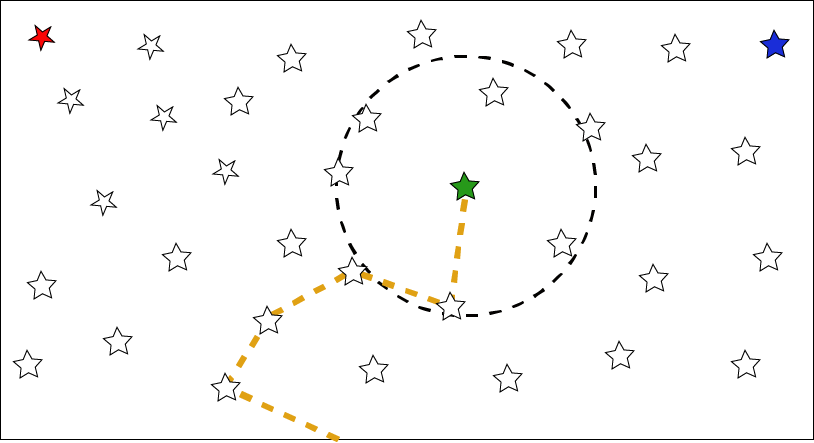
\includegraphics[scale=0.25]{Images/Map.png}
    \caption{First map mock-up used to communicate the basic concept to the team. The green node represents the position of the player, and the red and blue stars are nodes that need to be visited. The ring around the player limits the nodes that can be reached in one move, and the yellow line shows the already visited nodes.}
    \label{fig:map}
\end{figure}
\subsubsection{Board Game mechanic}
The \textit{Base Management} pattern is the next one that was chosen to create the analogue part of \textit{Archipelago}. The term \textit{base} refers to the central part of the game, that the players would use to travel from one node to the other. This pattern is closer to tabletop game mechanics, where the players uses the different resources available to progress through the game. As an example, the game \textit{Agricola} (Rosenberg, 2007) \cite{game:agri} illustrates this mechanic in various ways: the players need to improve their resources collecting capacity in order to manage their farm and their family. This create a progression based on the player's ability to manage resources correctly in order to produce more resources during the later turns in the game.

In \textit{Archipelago}, the resources would have different uses and origins. On the same principle, the various ways in which the base could be upgraded would provide a variety of gameplays and strategies, thus enforcing the "replayability" of the game.

\begin{figure}[!ht]
    \centering
    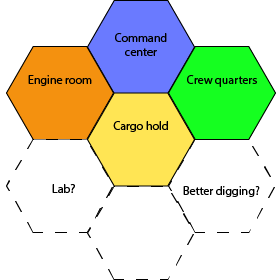
\includegraphics[scale=0.5]{Images/Base.png}
    \caption{Early mock-up describing the tiled structure of the base. Each hexagon represents an upgrade of the base.}
    \label{fig:base}
\end{figure}
\subsubsection{A collaborative board game}
By combining those two main design patterns, \textit{Archipelago} would merge mechanics specific to PCG-based with mechanics that could well be based on a game board, although not specific to the tabletop genre. An additional element from the tabletop game definition was then required to make the physicality of the game a crucial aspect of the game, and justify its \textit{hybrid game} denomination.

To make a successful combination of board game mechanic based on tiles and exploration of locations based on PCG, it was decided that \textit{Archipelago} would be a collaborative game. One single base would be shared by all the players. Designing the game as a collaborative board game would emphasize the social dimension of tabletop games. This is one of the thing that makes the board irreplaceable in the case of Archipelago. The board would provide an interface around which players can gather and plan the management of the base and the allocation of the necessary resources.

The collaboration would also enhance the PCG-based mechanics of the game in an original way. Indeed, games using this mechanic leave their player alone when evaluating the risk of performing or not an action. This time, the players would need to take the decisions together. This different approach would also bring another kind of flavour to hybrid games, and it was hoped that the discussion that would take place before performing the events would provide an enjoyable experience.
\begin{figure}[!ht]
    \centering
    \includegraphics[scale=0.5]{Images/Core_loop.png}
    \caption{A visual representation of the core loop, composed by the three different steps composing one turn.}
    \label{fig:loop}
\end{figure}
The combination of those patterns was the base of the core loop (see figure \ref{fig:loop}). The players would have to collaborate managing their base using the resources found during the event exploration. The events would be procedurally generated and only occur on the digital device. Building over such an abstract game concept required another brainstorm session to explore the possibilities offered by such mechanic, and exploit the digital component using PCG (see appendix \ref{fig:brainstorm2}). The inspirations found after the brainstorm session gave directions to explore potential hybrid game specific experiences.
\section{Designing \textit{Archipelago}}
As mentioned earlier, the PCG integration in hybrid games on a design point of view is explored via prototypes. Based on the prototyping methods and playtest results analysis explained in section \ref{sec:proto}, the game evolved towards a final state which encompasses all the different mechanics used to prove the interest of using PCG in a hybrid game. The most crucial aspects of the game supporting the research purpose of this paper will be described in this section.
\subsection{Game Setting}
In \textit{Archipelago}, the players have been sent by their King to explore a newly discovered archipelago of floating islands. They are commanding a flying castle that is powered by a crystal emitting energy. The castle is composed of rooms that each have a purpose in the game. These rooms range from \textit{Mining Guild} allowing the players to gather the required material for construction; to \textit{Mechanic's Workshop} to repair the rooms that are damaged during the exploration phase. The players have to fly from one island to the other in order to reach the final island on the map and finish the game. Islands are composed of different locations, which are generally filled with magic: magic crystals are scattered around the archipelago and with time created strange effects. The players will have to use Alchemy in order to extract as much resources as possible from the different locations. 

The archipelago is inhabited though, and the players will have to confront the different factions, sometimes by  allying; other times by betraying. The relation with the factions influences the outcomes in various ways, modifying the amount of resources that players gain, and affecting the game difficulty. The events then become more and more dangerous as the players progress and acquire a reputation in the archipelago.
\subsection{Early prototyping}
In the early stages of the development, it was necessary to test the core mechanic established before moving on to the implementation of the digital device and the PCG. A first prototype was created. The purpose of this prototype was to experiment the basic core mechanic around which the game would be built, and communicate this concept to the team.
\subsubsection{The first playtest}
\begin{figure}[!ht]
    \centering
    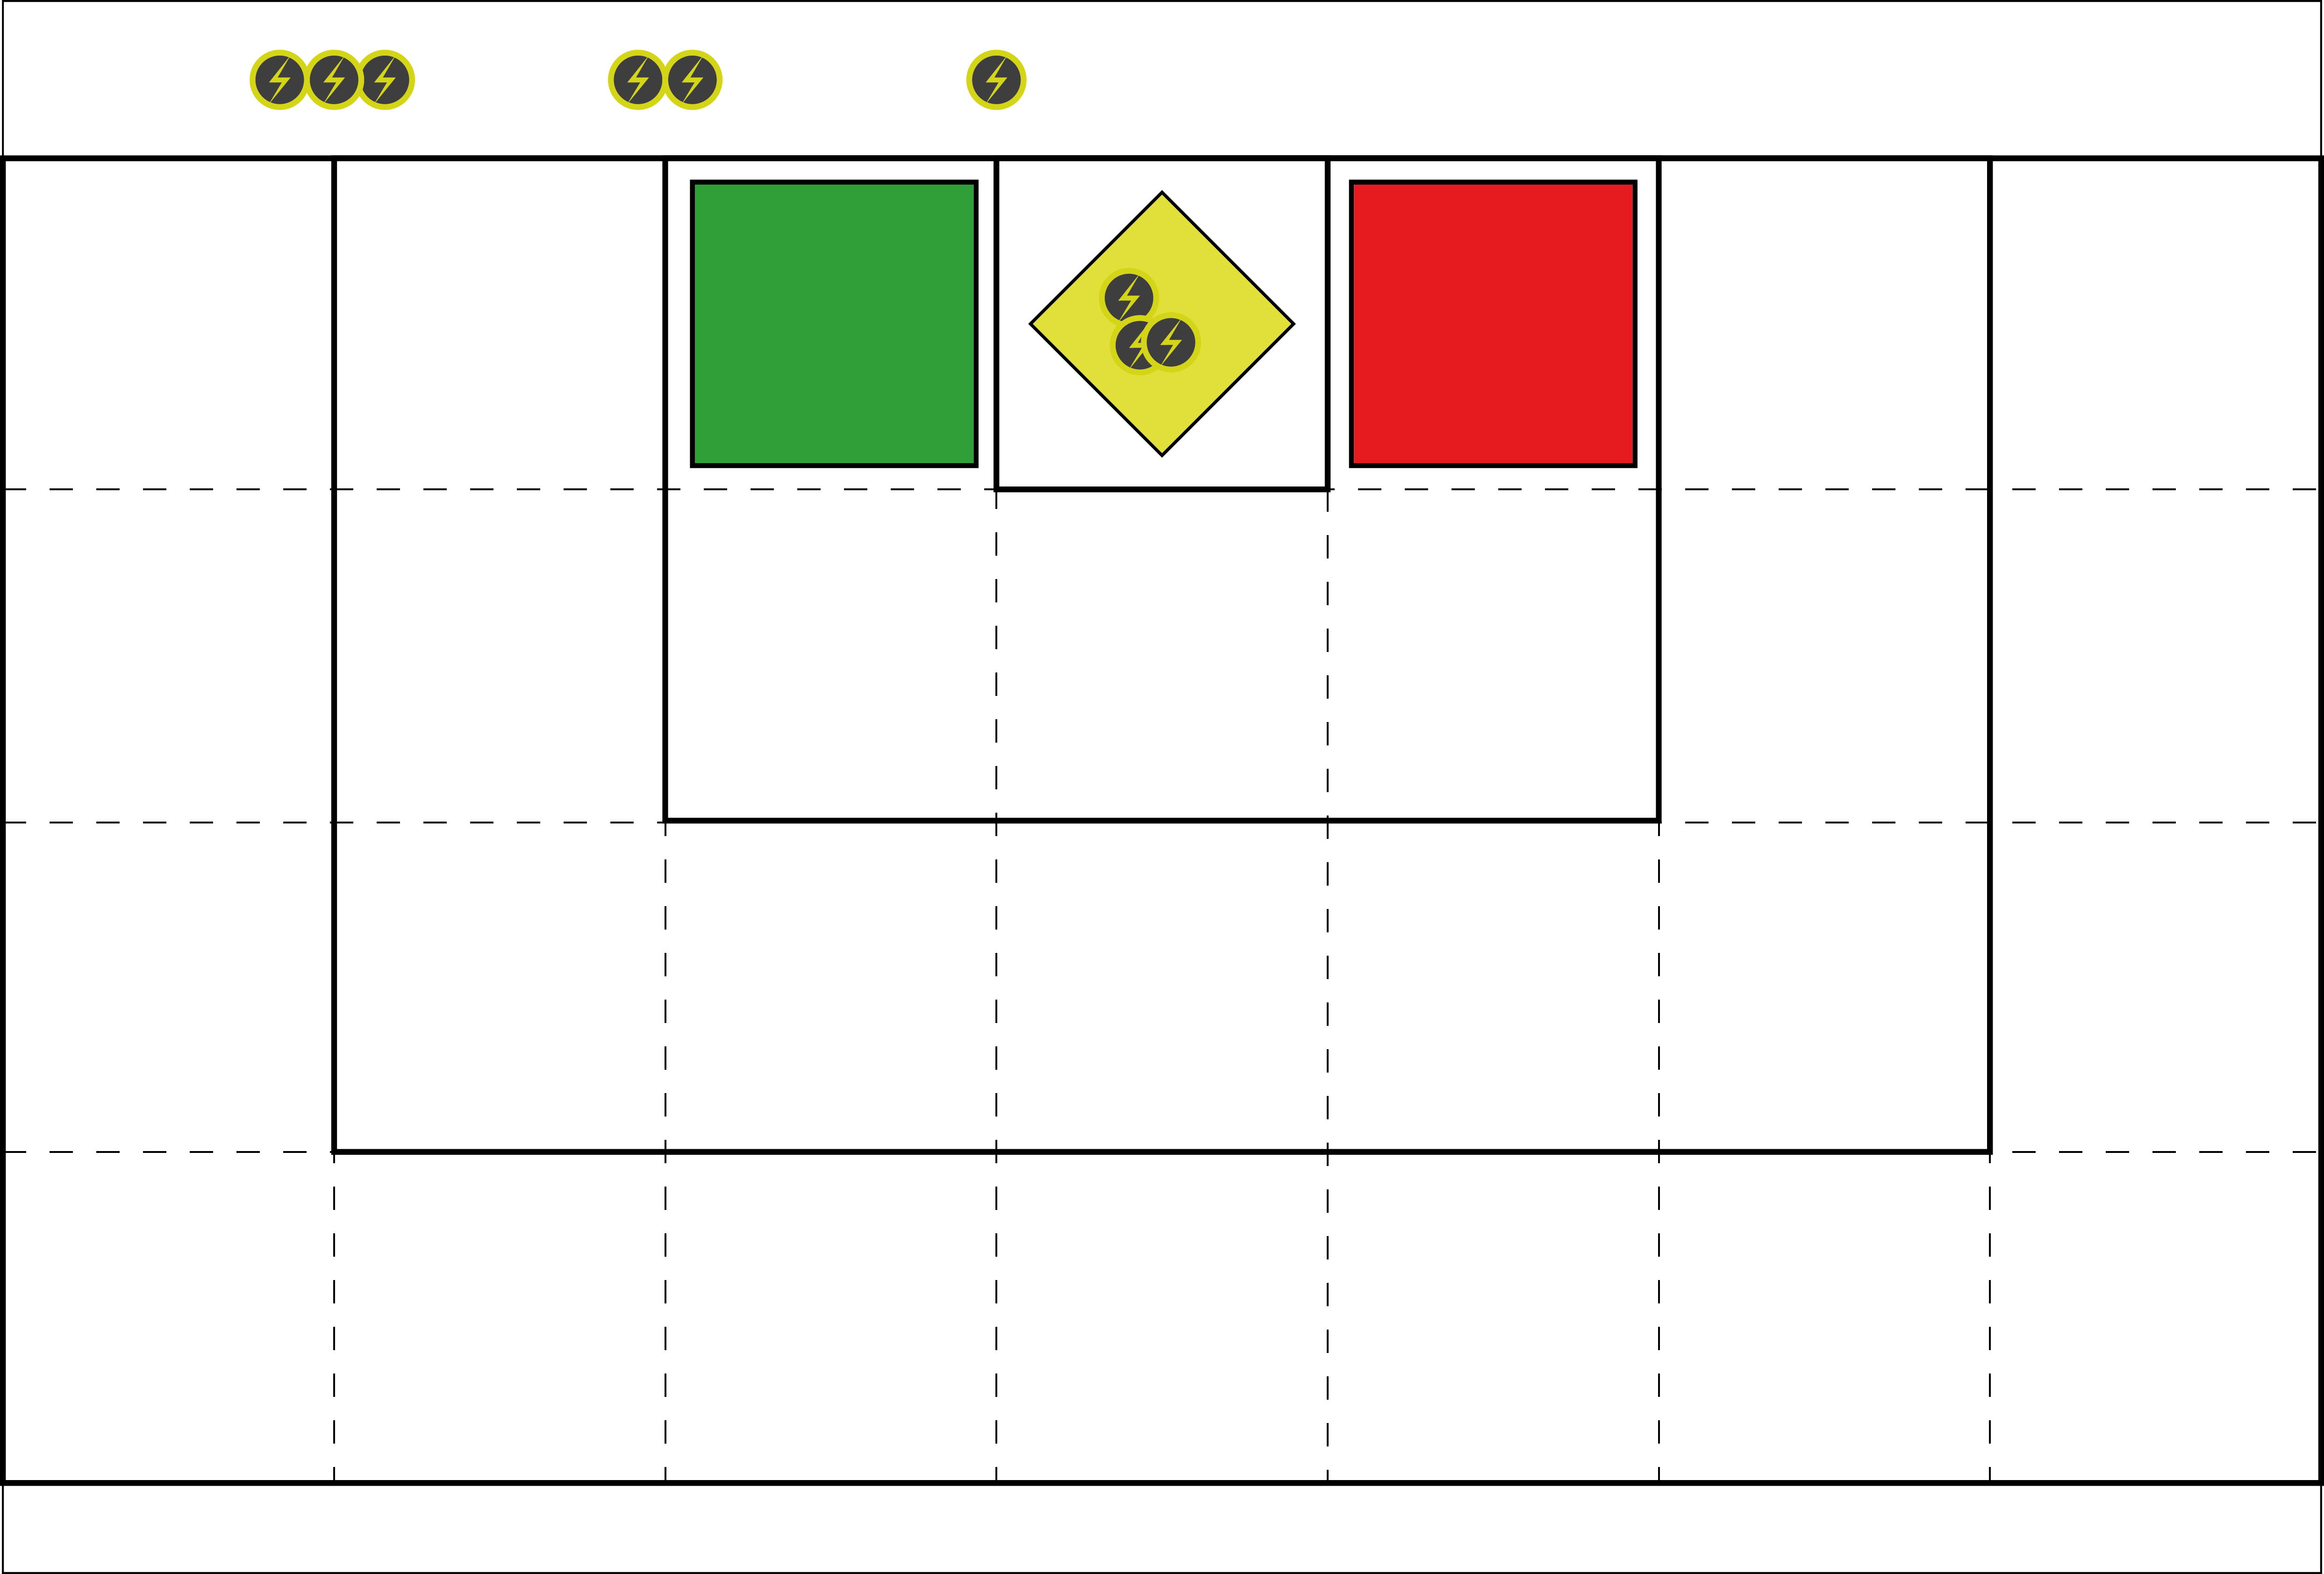
\includegraphics[scale=0.5]{Images/Board1.png}
    \caption{A representation of the base used in the first prototype.}
    \label{fig:base1}
\end{figure}
Based on Lim et al.'s framework to create relevant prototypes, the first iteration of \textit{Archipelago} is described by its main properties

Since it was one of the first version to be tested by players external to the team, the application using PCG was not yet ready. Therefore paper and dice composed the \textit{Material}. The paper was used for the representation of the base on the game's board and the dice were used to simulate the PCG part. This prototype had a low fidelity \textit{Resolution}. The representation of the base is very abstract and the digital component of the game was simulated.The \textit{Scope} included several elements: testing how the base should be represented on the board and how it should be managed, experimenting a basic resource system based on collaboration and providing an idea of when the digital component should be used in the game. 

The mechanic of the prototype contain several element. Refer to figure \ref{fig:base} for each description given below:
\begin{itemize}
\item The base is divided into squares, each square being a space where building a room is possible. \textit{Construction Zones} have to be unlocked in order to extend the available construction space. To unlock a zone, the players have to power the \textit{Core} with \textit{Energy} token. The amount of \textit{Energy} token required to access a construction zone is indicated at the limit between the two zones.
\item The \textit{Cargo Hold} tile limits the \textit{Scrap} players can have to 2 tokens per \textit{Cargo Hold} tile.
\item The \textit{Crew Quarters} limits the \textit{Crew members} that players can have to 2 tokens per \textit{Crew Quarters} tile.
\item \textit{Scrap} tokens, \textit{Crew member} tokens and \textit{Energy} tokens are gathered thanks to the \textit{Exploration Room}. To start gathering, the players assign a \textit{Crew member} to the \textit{Exploration Room} and roll a dye. Assigning two \textit{Crew member} tokens provides a second dye roll (see figure \ref{fig:Dicetable}). Gathering can only be done at the end of the turn.
\begin{figure}[!ht]
    \centering
    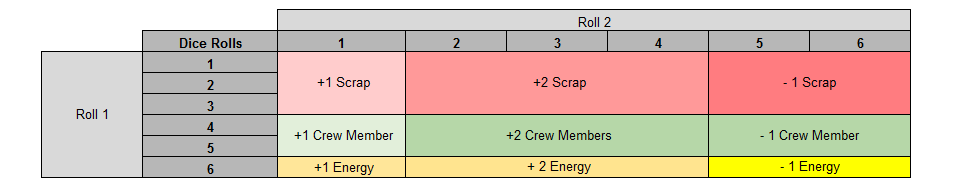
\includegraphics[scale=0.6]{Images/DiceProto1.png}
    \caption{Table representing the results of the dice rolls. One dye only gives access to the leftmost column of results. A second dye gives access to better rewards, but there is a risk of losing resources. There is still a chance to get a standard reward with two dice.}
    \label{fig:Dicetable}
\end{figure}
\end{itemize}
\subsubsection{Feedback}
Feedback from the first testers showed that even with abstract components, the flow of game provided a sufficiently good base for discussion. According to playtesters, dividing the board in \textit{Construction Zones} was also an interesting mechanic in itself but it appeared several times that the players were stuck with not enough resources to play. It needed to be refined. The randomness of the result (due to the use of dice) also showed the problem of engagement in the game. This emphasized the notion of player control tied to PCG-based game design. Using more than one parameter proved that the players needed to feel their influence on the generation of the rewards. It happened that one player tried to convince the others that using two dice would be more efficient. This also showed the importance of player specialization in the game. 
Finally, it gave a good idea of how the flow of the game would be. It was decided to build the work over this to start implementing the PCG and the digital device in the game.

On the bases of the first playtest, it was decided that a turn in \textit{Archipelago} would be divided in two different phases:
\begin{labeling}{Management Phase}
\item[\textbf{Management Phase}] The phase during which the players discuss and allocate the different resources in the most efficient way. This phase is based on the physical components, gathering the players around the board and using the game pieces.
\item[\textbf{Exploration Phase}] After the management phase, the players chose an island to explore on the device. This island contains locations to visit, and situations to overcome. The choices made by the players condition the amount and nature of resources they are getting. The PCG would generate the island, the choices 
\end{labeling}
As previously mentioned, one of the challenges of making \textit{Archipelago} was to make both digital and analogue aspects of the game support each other without interfering play as well as being essential in the game. This idea followed the whole design process of the game.
\subsection{Replayability}
The first aspect generally cited to enhance the play with PCG-based game design is replayability  the notion of replaying the game without facing the same situations. One of the crucial aspect of \textit{Archipelago} is to exploit PCG to generate the income of resources supporting the collaborative tabletop gameplay. The design of the event generation system was then an important part of the development and is the first element that will be described here.
\subsubsection{An infinite number of events}
After simulating the event generation system with dice, the first iteration of the event generation system was included in the \textit{Scope} of another prototype. As observed during early prototyping, the number and quality of parameters selected to create those events and their outcomes was an important part of design. The prototype should then introduce those parameters both to the players and to the development team. Prototyping the event generation should then help manifesting two main design problems:
\begin{itemize}
\item Finding the right number of parameters to use in order to generate a content in which the patterns of the event generation system would not be recognized by the players.
\item The parameters should also be coherent both in a technical perspective, as well as being recognizable by the players so that their decisions could be based on those parameters
\end{itemize}
\subsubsection{A flexible board game}
\subsection{Player control and Adaptability}
\subsubsection{Diplomacy system}
\subsubsection{Risk and Reward}
\subsection{Specialization and collaboration}
\subsubsection{Constructed Specialization}
\subsubsection{Encouraging Collaboration}
\subsection{A hybrid game}
\subsubsection{Merging Analogue and Digital}
Mainly, the function of the application is to contain all the information regarding events, movement, factions and the overall data available within the game. The application is the only connection the players will have to what is happening in the game, as without it, the game would just be an empty board with pieces that would have no purpose. 
When playing the Archipelago, the digital part of the game, the app, will provide the players with a layout of the world, i.e. the map with all its islands, and it will contain all methods of receiving rewards as well as receiving penalties for executed events. It determines which resource the players will receive, what the "story" is, in terms of flavour presented, and it contains the factions and the players standing with each of them.
The events in the app, are made to be like cards that the board game would have, if there was no app. But by having the digital computing and memory, the diversity of these events are much greater and there is no need for a huge pile of cards and expansion packs to generate different and diverse events. The app is in full control over what the players get and what is taken away from them, and given that there is now memory in place, the possibility to create new content based on previous events is there. Another part that the application plays in the entirety of the game, is that it controls when effects take place. If there has been an event with a specific outcome, it is then the system that controls if there should be consequences based on those outcomes. If there was no digital application in place, there would have to be a large amount of cards and pieces in the board game, along with very specific rules and combination guides, for the players to sufficiently be able to piece together new events and outcomes. So the biggest purpose of the app, as implemented in this solution, is to have complete control over all actions, story, events and outcomes and be able to present them to the players without using much time, which the players would do if they had to combine their own "gameplay".
\subsubsection{User Experience and Interaction Design}


\section{Development Structure (Technical)}
This part of the paper will go into more detail on how the development of the project went as seen from a more technical aspect. This includes the making of prototypes, the way to go from communicating with a designer to implementing a solution, and lastly problem solving along the way.

\subsection{From design to implementation}
When working as a developer, you also work closely with the designer. What we did during our development period, was to get the wants and needs from the designer, and try to implement it into prototypes for overlook and feedback. 
If things needed to be changed, added or removed, the team would go through in general terms what needed to be done, and then the requested adjustments would be made to the prototypes.

In the next part of this section, we will go into more detail on how the prototyping would take place, how the communication between programmers and developer happened, and what changes were made over time during the period of development.

\subsection{Prototyping (Application)}
Right from the start, it was important to quickly produce smaller prototypes so that we could get an idea of how to continue, and to test the implementations that were made. The first part of the project is to set up the app and have a starting point that you can build on. In our case, this meant an initial screen with a simple UI that could be added to, moved around and overall that could display text and data. On top of that, the backbone of the system would be to have different data classes that could contain the various sorts of information that would be needed.

\begin{description}
\item[Prototype 1:] A simple UI with text boxes, buttons and a simple data manager that contains the initial values.
\end{description}

Going onwards, designer and programmers alike, would come with inputs to set the foundation for which data types would be needed in order to produce the desired results.
It was decided early on that there would be events that the players could interact with, and that these events would have board pieces and flavour text associated with them. The basic layout for the \textit{flow} of the game is then set, with the idea that there would be a main world scene where all the destinations would be displayed, and each of these destinations would have their own scene where the locations possible would be shown.

\begin{description}
\item[Prototype 2:] Now the application has a main world screen with a multitude of destinations would be displayed in the form of simple spheres that can be clicked. When clicked, the destination scene would be shown, which contains the simple representation of locations, also in the form of spheres.
The map layout is generated by using an L-system algorithm\ref{sec:lsys}.
\end{description}

At this point, the need to link the application with the board game occurs. A player object is needed within the application, and it needs to be able to move around the world space. Also the initial event structure is taking form, which means there is a need for the data to be constructed along with some dummy flavour to be shown on the screen.

\begin{description}
\item[Prototype 3:] Introducing the player object, the event class and XML files with the initial flavour texts.
\end{description}

The events and the data contained is rather simple at this point. An event is mostly consisting of a simple description, a set of premade options, and one or two outcomes that are also premade. So a few events were made by selecting different descriptions, along with randomly selected options and an outcome for each option.

With the backbone in place for creating \textit{varying} events, the next logical step, is to start coming up with the algorithm for how the events should be constructed and generated (the actual algorithm for how it works can be seen in section \ref{sec:eve}, \textit{Events}, later in this document).

\begin{description}
\item[Prototype 4:] With a better working event generation system, the next prototype is made with a wider array of option possibilities, along with more outcomes.
\end{description}

So now the basis for the events are in place. The next part of the application, will be to have a more diverse collection of flavour texts.
This meant that we would have to come up with how the flavour text should be combined (see how in section \ref{sec:flav}, \textit{Flavour of the Events}, and in section \ref{sec:disc}, \textit{Discussion}, later in this document) and create an algorithm for doing so. 

\begin{description}
\item[Prototype 5:] Event generation is in place along with flavour-combining algorithm. Everything seems to be working as intended, with the exception of some bugs here and there. But the overall main event system that allows the first play through of the game, is now in place.
\end{description}

After going through some plays of the game, and as more design decisions are made, more functionalities have to be implemented. The next step in the prototyping cycle would be to get a faction system going. What this would mean on top of the actual faction system itself, is that there would have to be changes made to the flavour combinations, as the resulting texts would now have to include the factions. Furthermore, there would have to be special events and rewards/results from events, that would affect the reputation the players would get with the respective factions.

\begin{description}
\item[Prototype 6:]
The faction system is implemented, along with a set of special events and outcomes that can be triggered via the regular event system. Now an event can have a 3rd option, which will have the chance to trigger the special events. There are 2 types of special events implemented, the first is a faction-war event, which would let the players choose sides between factions, the second type is the big ones that are based on previous experiences and encounters that the players have had within the game. When the 2nd type of special events are selected, it will take various data from the event that triggered it and use those in special combinations to give the players the experience of \textit{history} and \textit{consequence}.
\end{description}

By now, the application has most all of the structure and algorithmic computation and generation needed to make the game a complete experience.
The remaining tasks to be solved, is implementing better visuals, icons and signifiers. Scaling the elements to fit the tablet on which it will be played, and making sure there are as little bugs as possible.

\begin{description}
\item[Prototype 7:]
The final product is ready. No more coding and algorithmic calculations are needed. From this point in, polish is the keyword. Optimizing the feel of the application, making sure everything runs smoothly and looks good, and having as many flavour text pieces as possible for every element, so that the game will be as diverse as possible.
\end{description}

\pagebreak
\chapter{Technical overview}
In this chapter we will elaborate on how the application for \textit{Archipelago} is constructed, the structure of the app and the scenes contained within it and how they function. After that, we will go into more details on the UI elements and user interaction, as well as how the users can interact with and move around the viewport to better get an overlook of the map, and this will lead on to the world map itself with its layout and how it is constructed. This is followed by a detailed description of how the PCG algorithms work and how the events with its options, outcomes and flavour is constructed. In the end of this chapter we will go through the app in action from start to end and how it is utilized together with its features.

\section{App structure}
This section details the overall structure of the app.
First the scenes in their structure in the game and later the UI and additional elements.

\subsection{Scenes}
\label{sec:scen}
This section is dedicated to the overview of the technical relation between the different scenes and their individual purpose. Each scene will be detailed in each of the following subsections going from the first scene in the app, to the last scene.
The transitions between the different scenes can be seen in the overview presented by figure \ref{fig:appState}. The names on the transitions are related to the button presses which initiate them. 
The diagram does not show any of the actions which transition to the same state.

\begin{figure}[!ht]
    \centering
    \includegraphics[scale=0.5]{Images/StateDiagram.png}
    \caption{The overview of the scenes in the application and their linkage. The diagram shows each of the actions which change to other scenes.}
    \label{fig:appState}
\end{figure}

\subsubsection{StartMenu}
As the game is started, you immediately enter the start screen. This is a simple scene containing only the button that says "Start Game". The purpose behind this scene is to let the users be able to chose when they want to start the game, so that they are not necessarily overpowered by the rules of the game (board game part) and the visuals of the app itself when started.

Furthermore, as this scene is loaded, the preliminaries to the world generation and the loading of required data from XML files is handled. This minor loading, takes some of the load of the rest of the program, giving an overall smoother experience.
This includes the general l-system structure, which is run in the start menu, the loading of board game pieces, and the loading of the different factions in the game.

As soon as the "Start Game" button is clicked, the app will initialize the contents of the world, and present it to the user within the next scene, which is the WorldScene.

\subsubsection{WorldScene}
\label{sec:worldscene}
This is the main layout of the world. It contains all the locations that the players can travel to, and shows them where they are, where they have been, and where they have to go.

When you first see this part of the program, you will notice that it has floating islands with rings around them, as well as a flying castle. The castle is the piece the players control, and it is what the board is representing in the physical part of the game.
At first glance, you might not see all of the map and all the different islands you can travel to, but by simply zooming out, the players are able to get a better view of the entire map layout, and from there, they can plan their chosen way. There is also a little arrow in the lower right corner of the screen, which always will point towards the goal-island. 
In figure \ref{fig:worldSc} you can see the scene which meets you once the scene is loaded.

\begin{figure}[!ht]
    \centering
    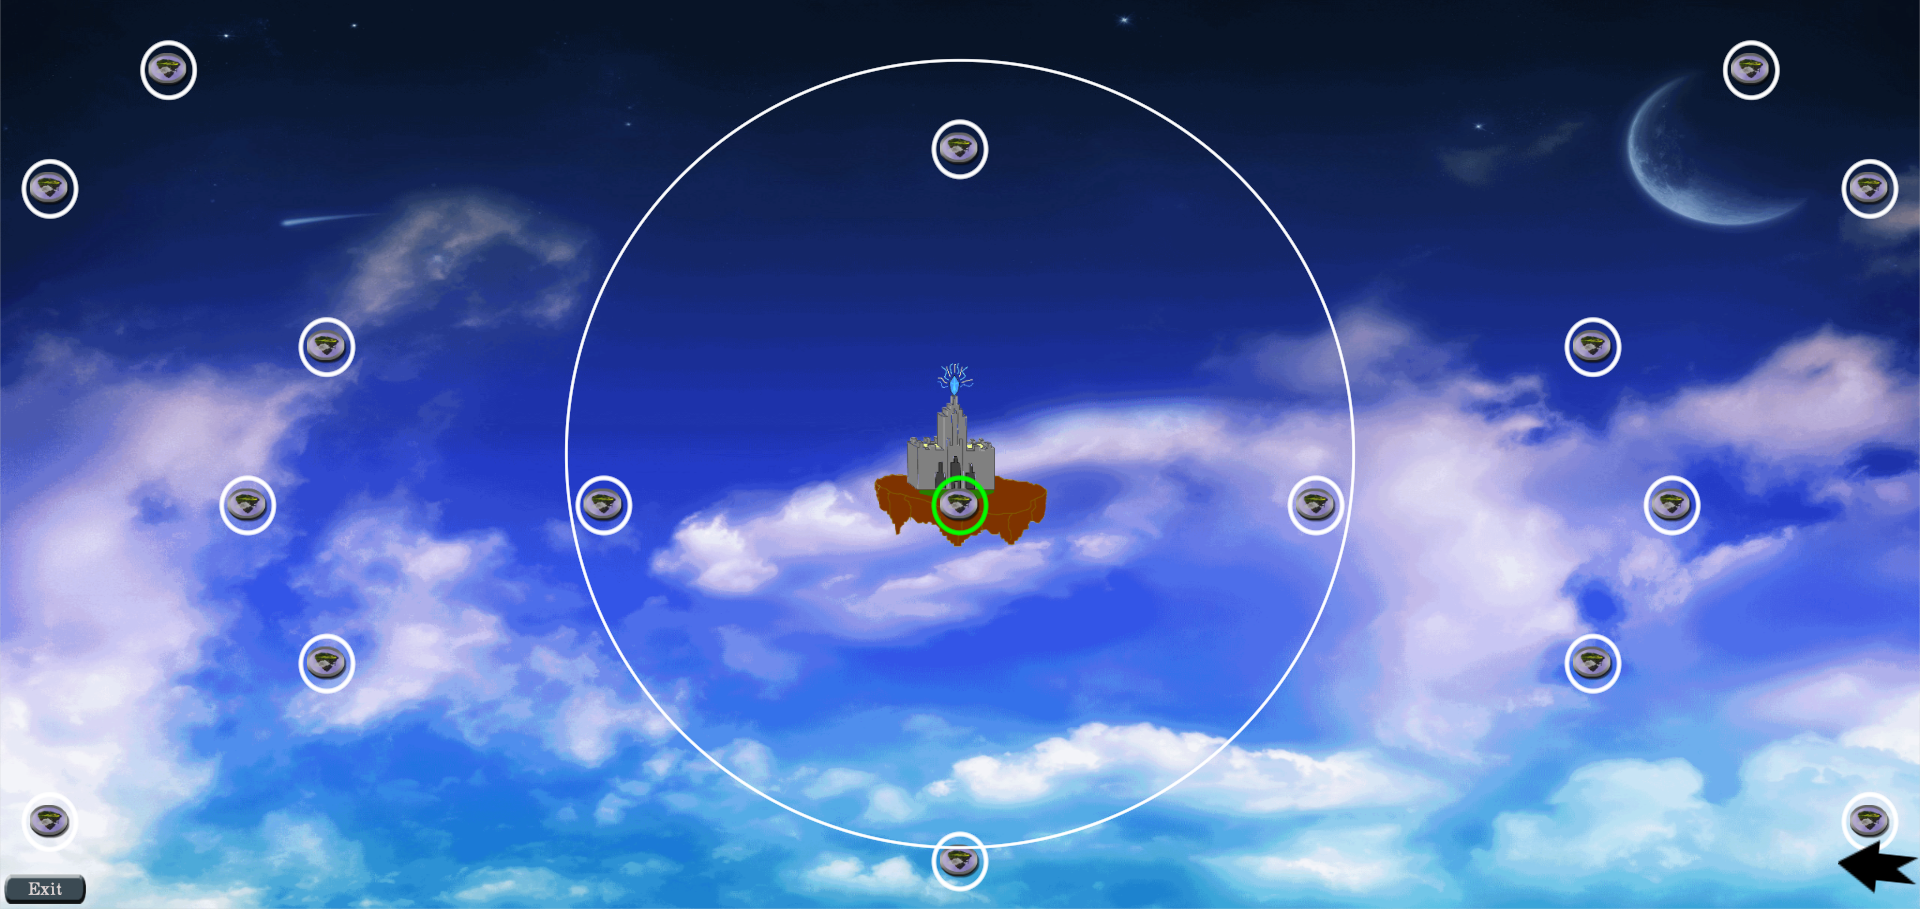
\includegraphics[scale=0.3]{Images/WorldScene.png}
    \caption{The WorldScene as seen on the PC version of the App. In the center the player token is represented as a floating castle. Also seen in the center is the green node, denoted as the starting node. In the lower right corner is the arrow pointing towards the goal node. The outer white ring indicates the maximum travelling distance of the players.}
    \label{fig:worldSc}
\end{figure}

As seen in the figure, there is a large white ring centered on the castle that the players control. This ring is indicating the range that the castle can travel in one turn of the game. Any islands that are within this ring, are available to be travelled to.
When travelling from one island to another, the ring around the island you arrived at will change color (from the initial white color). This signifies to the players that they have already been to that island and therefore do not necessarily have to go back to that place again unless they choose to do so.

When you click an island on the map, you will be faced with a pop-up box. This box is containing the name of the island, and a piece of text that somewhat describes it; flavour text. The box then has 2 buttons, or choices, either "exit" or "travel". If you exit, the box is closed, and you are free to choose another island to travel to. If you click travel, however, your castle will be moved towards that chosen island and stop once it reaches it. 
Once the castle has reached the island and the collider on the object is triggered, the app will move on to the NodeScene, where the island that you travelled to will be represented.

\subsubsection{NodeScene}
\label{sec:nodeScene}
The NodeScene is probably best known as the "island scene" or "event scene", because this is the scene where all the events take place, and it is the main place where the players will have to interact with each other in order to choose their wanted event.

Once this scene is loaded the events for the given island and the locations on it, are generated. The events uses the information from the world node in order to create the events. The reason the event generation to be moved to this location, were to limit the computing power required to initialize the world node. 

\begin{figure}[!ht]
    \centering
    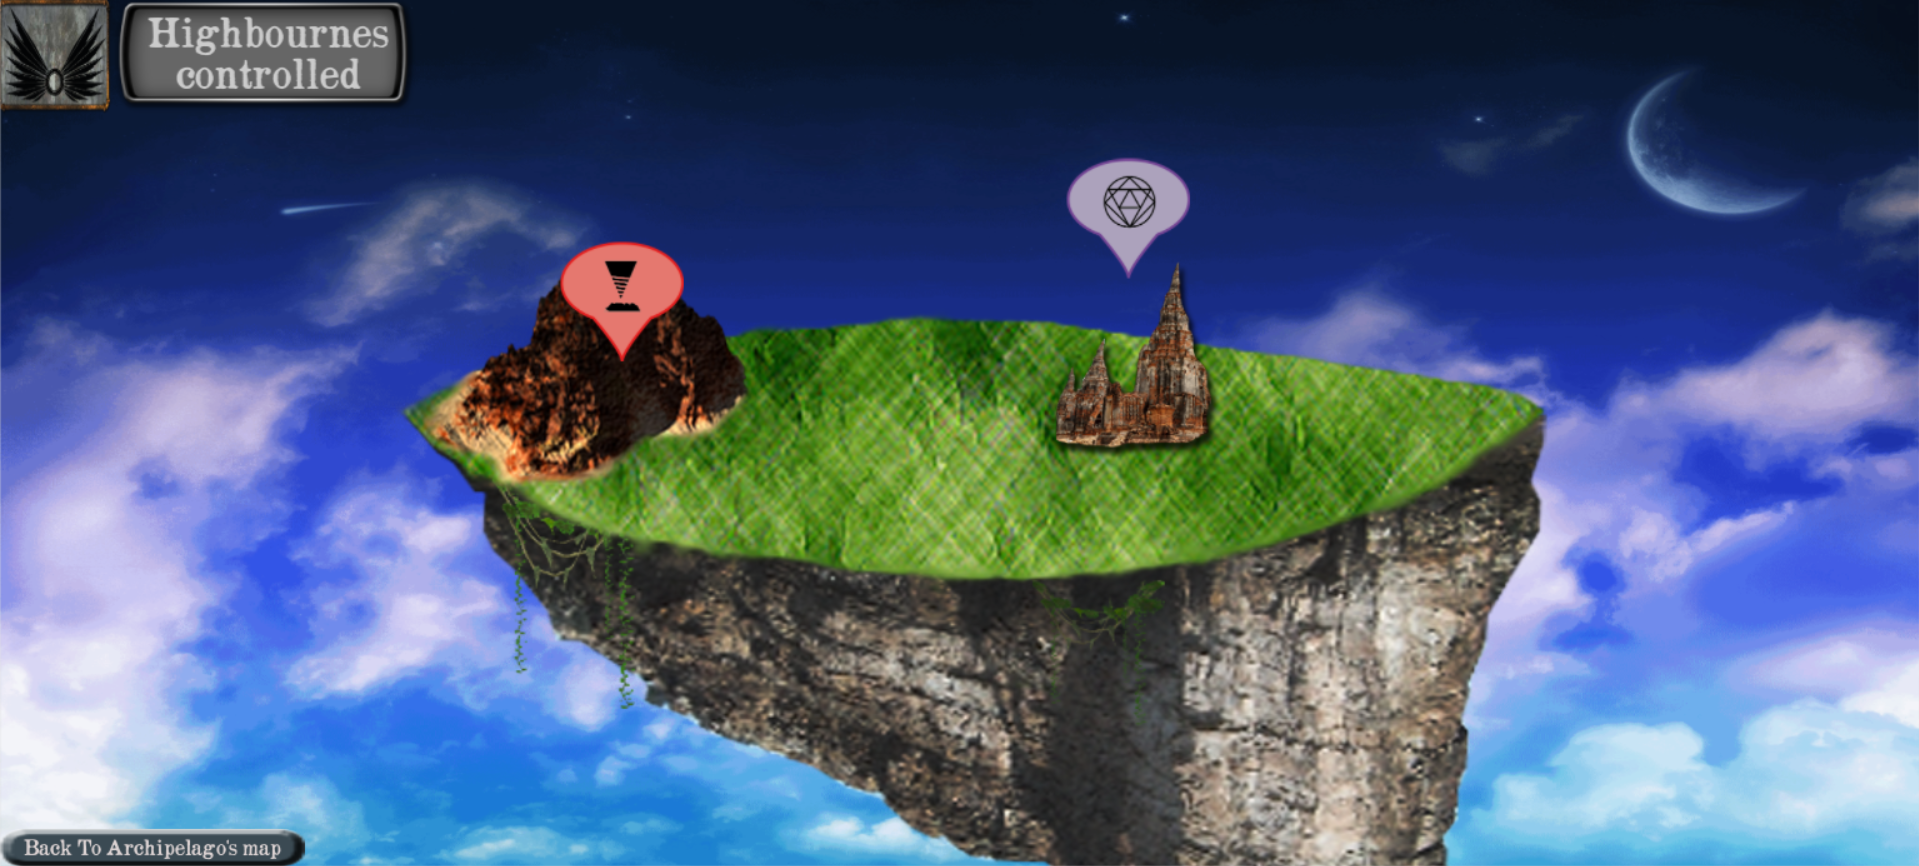
\includegraphics[width=\textwidth]{Images/NodeScene.png}
    \caption{The node scene as seen on the computer version of the app. In the center is the island, with two locations situated on it, a mine and a ruin. In the top left corner, it can be seen that the island is controlled by the Highbourne.}
    \label{fig:nodescene}
\end{figure}

In figure \ref{fig:nodescene} you can see one of the configurations that the island can have on generation. The island has two locations for the players to explore, a mine and a ruin. 
Each time an island is generated, it always comes with two locations for the players to visit, one for gathering and one for research. The gathering event will have a red icon with a drill on it hovering above the given location, whilst the research event will have will have a blue icon with a alchemical symbol.
Research events usually yield more alchemy points, whereas the gathering event has their basis in building materials.

Each island also have a general faction which in charge of all the locations on the island. Their icon and their affiliated symbol is located in the top left corner. From this the players are able to easily identify whether they have arrived at a location where they have allies or enemies, and from that conclude whether their events are going to have a higher chance of success with better outcomes, allied faction, or if there is going to be a higher chance of failure with worse outcomes, enemy faction.
The faction is also displayed on the travel panel presented in the WorldScene, giving the players the opportunity to choose which factions they wish to interact with.

\begin{figure}[!ht]
    \centering
    \begin{subfigure}[b]{\textwidth}
        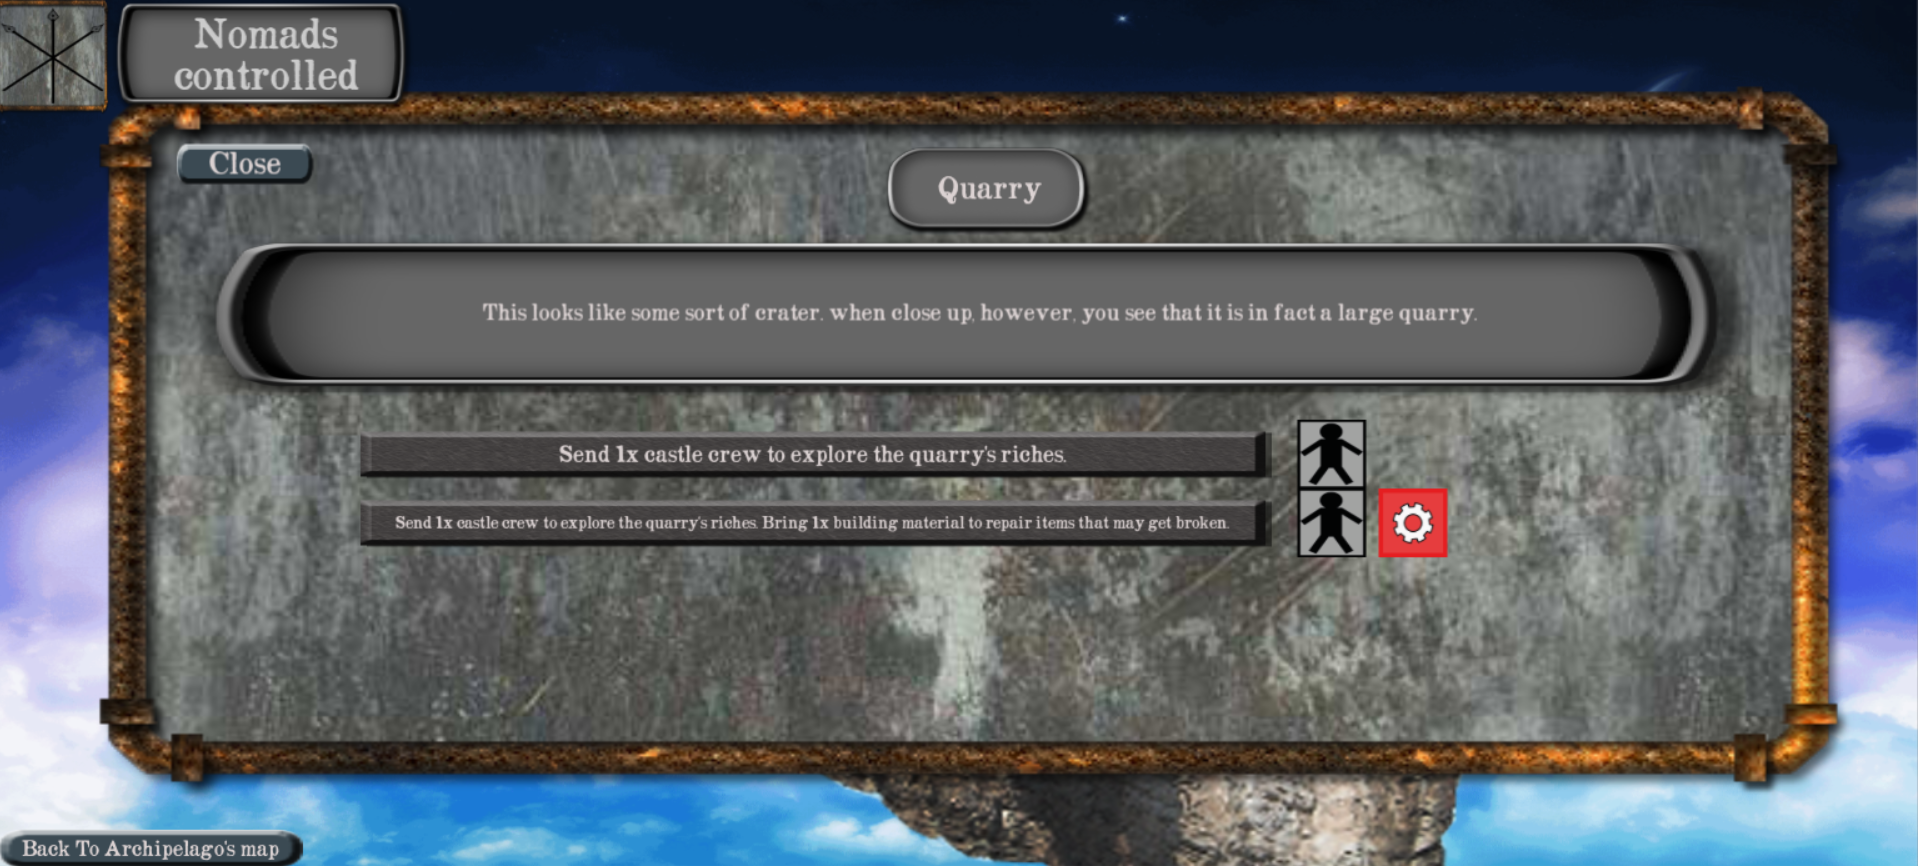
\includegraphics[width=\textwidth]{Images/EventPanel.png}
        \caption{This is the panel related to the event of a location the players have chosen to explore. In the top of the panel there is the name of the location which the players are exploring.
       In the middle of the panel is the buttons which resolves the event, with the requirements of the event represented as images next to the button.
        Above the buttons is a short description of the event, referred to as flavour text. If the panel was opened by mistake, the panel can be closed using the associated button in the top left corner. }
        \label{fig:evepan}
    \end{subfigure}
    \begin{subfigure}[b]{\textwidth}
        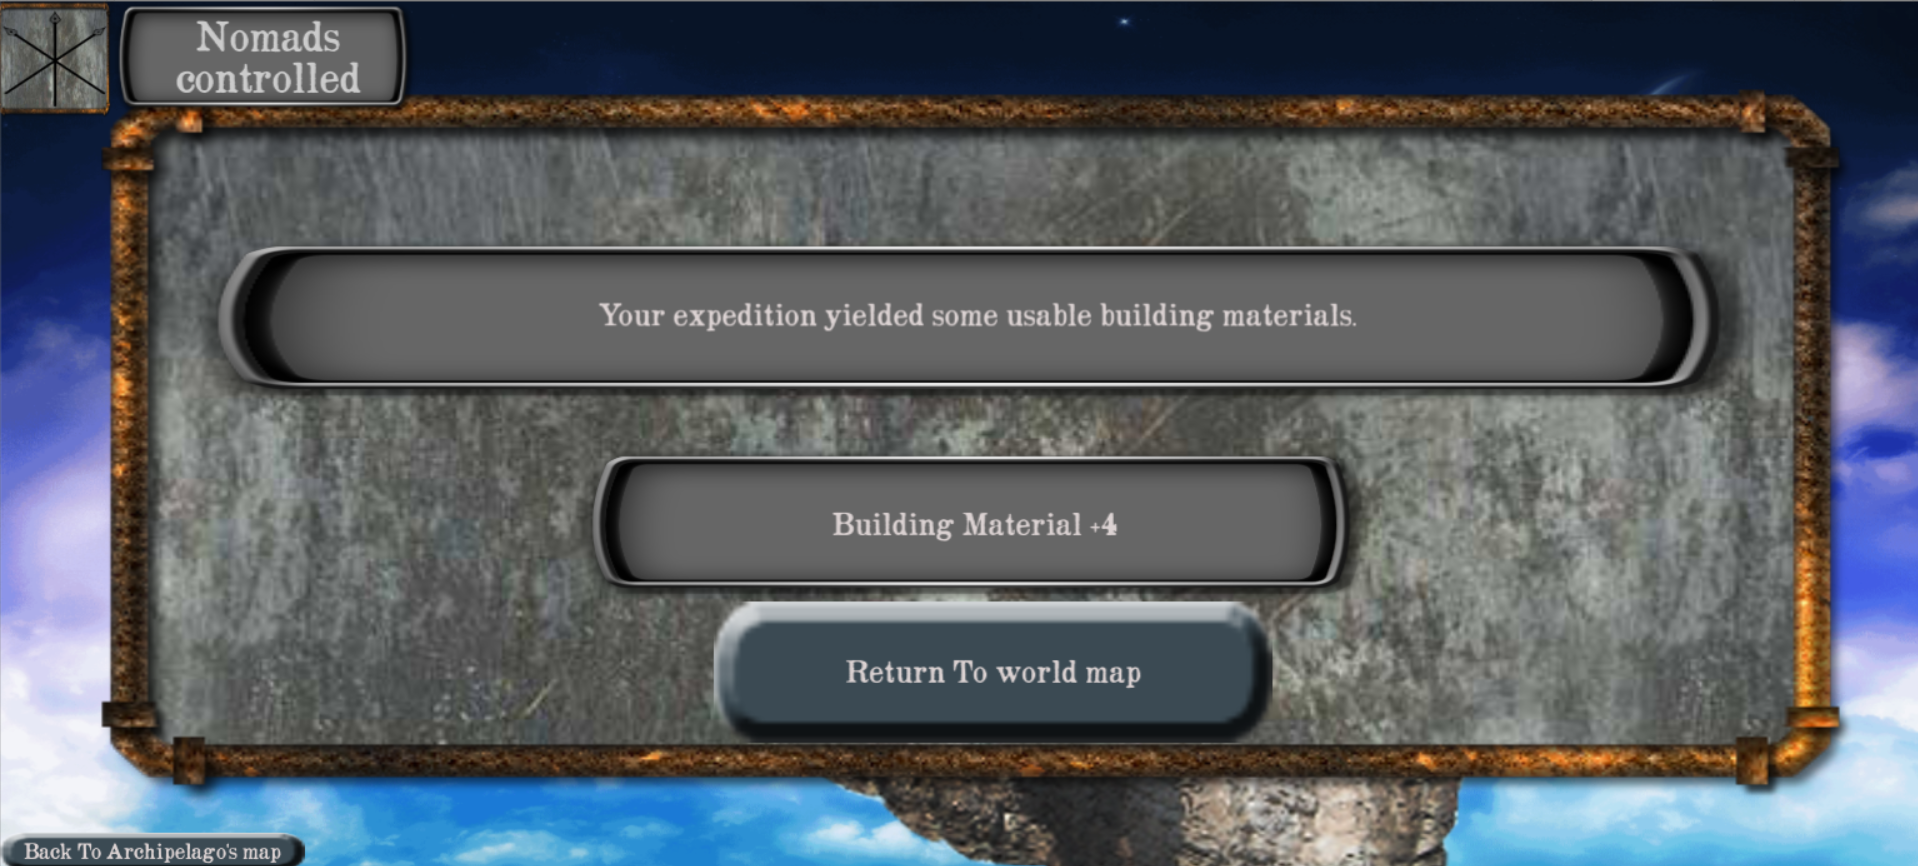
\includegraphics[width=\textwidth]{Images/EventResolution.png}
        \caption{The panel related to the resolution of the events. The panel comes with a short flavour text about what has transpired, followed by a list of the gameplay objects which have been changed in the event. The panel can be closed by clicking the return to world map, ending the scene and initializing the WorldScene.}
        \label{fig:everes}
    \end{subfigure}
    \caption{Images of the different panel in the event execution.}
    \label{fig:eventPans}
\end{figure}

Once an area of the island has been clicked, a confirm box will be shown where the player will have to confirm that this is the area they want to explore. 

Once the explore button is clicked, the panel in figure \ref{fig:evepan} will appear. 
This panel displays the location you have chosen to explore along with some flavour text about the location. 
The panel will come with either 2 or 3 options, in the example there is only two, represented as buttons below the flavour text. 
Each option have one or more requirements, which a both included in the flavour text on the button and displayed as images next to it. These requirements are the resources the players must commit in order to resolve the event. 
E.g. "Send 1x castle crew to explore the quarry's riches. Bring 1x building material along to repair items that may get broken.", tells the players that they need 1 castle crew and 1 building material to commit to this option.

Once you have selected an option, the panel will shift to the resolution panel as seen in figure \ref{fig:everes}. The event is concluded and the players is presented with the results of their choice. The result comes in the form of a flavour text describing what happened, and a list of either rewards or penalties.
Once the players close the resolution panel, they will return back to the WorldScene, ready to move on to the next island.

\subsubsection{ScoreScene}
Upon reaching the final island in the WorldScene, the one island with the blue ring around it and that the arrow, that was mentioned earlier, is pointing towards, the game ends. 
What happens then is that all the data is cleared from the app, the WorldScene shifts to the ScoreScene, and the players are presented with an end text that basically tells them that they reached the goal. This scene also includes a button that takes the players back to the StartMenu where they can play another game if they so choose.

\subsection{Buttons and Raycasting on images}
The players main source of interaction is via the use of buttons and images. The buttons that can be found on the main screen, on various events and dialog boxes, all have their own respective functionalities connected with them. One button might close a box, another might start the game, each button have specific actions that they perform, and what they do or how they affect the gameplay, is represented on them either via specific text, flavour text or icons.
The images and icons are a bit more tricky, especially for the players, as they do not necessarily signify to them that they can be interacted with, unlike the buttons which most people instinctively know does something.
By programming itself, an image is just an image. It has no function attached to it, and does not do anything specific other than portraying a picture. So in order to make the images \textit{clickable} you have to introduce raycasting.

Raycasting is when you create a line from one point to another, and in this case the only logical way to raycast to the images, was to make the initial start point be wherever the user touch the screen. So when the screen is touched, and the initial position is set, a ray will be made from that point and go \textit{into} the screen (the z direction). By doing this, we can calculate if at any point of the ray, it touches an image that we want to give functionality. If this is the case and say that an exploration location is colliding with the ray, the application will then know to execute the functionalities that that images is holding. In the case of a location being clicked, an event box will appear and the players can continue with the game, and explore on.

In the next section, the UI Elements section, you will be introduced to all the remaining elements that is used in the digital part of the game.

\subsection{UI elements}
In this section, we will go through all the different UI elements within the app and explain in more detail their purpose and how they work.

\subsubsection{Boxes}

There are a number of different boxes that will appear over the course of a game session with this app. By "boxes" we refer to the dialog boxes that pop up when interacting with different elements of the application itself, e.g. an event popping up when interacting with an island.
The purpose of each box on a high level, is to convey information to the players, be it information about the location that they are travelling to, or the results of an event they have just completed.
Each box has it's own purpose, but as just stated, the main purpose is to convey information. The first box that appears when interacting with the app, is the "travel confirmation" box. This box tells a little information about the island that the player wishes to travel to, like the name of the island, and a few lines of flavour text that goes with said name. It also contains two buttons; one for accepting the travel location, and another one cancelling.
Once you have travelled to a location the next box will appear when the region the players want to explore is clicked. This box, like the one before, has a name (the location type like "mine") and a text field for the flavour about that mine. Again there is a button for accepting, and one for declining. 

Next up, you have the event box. This is the main box of the game, one might say. It contains a text field where the procedurally generated flavour text is displayed, along with 2 or 3 buttons that has the options for completion that the players may choose from. 
Once an option has been chosen, the application loads the result box. This box is mainly a field where the description of what happened during the event is shown. it also has a field where the results in terms of board pieces gained/lost, reputation changes, etc. are shown. In addition, it has a "return" button, where once clicked, the players are taken back to the WorldScene where their game continues.


\subsubsection{Faction icons}
The faction icons have a rather small visual part in the application, but the impact it makes on understanding the game and seeing what opportunities and rewards the players might get, is rather substantial. In the top left corner of each NodeScene screen, there is an icon that conveys to the players, which of the current 3 factions controls the island that they are on. With this information, and the information that the players might have a specific standing with said faction, allows the players to mentally make an image of what the outcomes of the event might be, in terms of good, bad or neutral.

\subsubsection{Buttons}	
The buttons in this application is the main way for the users to interact. If it is not the ray-casting and clicking on the islands in the world scene, the only other physical interaction with the application is through the buttons. The beauty of the buttons is that it allows the game to be rather easily built on to other platforms, such as android or IOS. The button has two main functionalities; the first would be to navigate within the app itself, like accepting to travel to one place, or closing one of the dialog boxes as described earlier. The other one is that the buttons themselves have a text field on them. By taking use of this feature, we are able to give the buttons meaning, in terms of carefully choosing what to display to the users. In the event box, there are between 2 or 3 buttons that holds options for how to solve the given event, and that means that we can set the text on the buttons to tell the players what each option will cost or require, e.g. one option can be to send out 1 of your crew to explore, whilst another option can be to send out 2 crew plus a cleric. Using precise and to-the-point text on the buttons allows the players to quickly understand what is required, and will allow for discussion to take place as to which one is the best option for the current state of the game.

\subsubsection{Islands}
The islands are the centre of the World Scene. All of them contains individually unique events that differ from each other. Each island is also controlled by a faction and as the players might get different standing with different factions at any given time in the course of a game, each tailored event will have a range of different outcomes depending on the players' standing with the controlling faction. 
As the main goal of the game, within the application, is to reach the goal node, it is important that the islands are spread around the world in a way so that the players themselves can choose which route they want to take in order to reach it. Be it the shortest way, or a longer way that requires more exploring and will take a longer time. Each island also have their own name and flavour to them, so that it hopefully will feel to the players that they have a history and a meaning.

\subsubsection{Castle}
The castle is the center piece on the table. The board in itself is a layout of the castle as represented within the application.
When moving around in the generated world, you move your entire castle. The castle is basically acting as the player object within the game. Since this is a collaborative game, however, it is up to the players to discuss amongst themselves how to use and distribute the resources that are \textit{contained} within the castle, and use their own minds to select how an event is to be resolved when the castle is entering an island.

\subsubsection{Rings}
As introduced in section \ref{sec:worldscene} in the worldscene, the rings are indicators of travel possibilities.

Every island on the map has a ring around it. The color of the ring indicates whether the island is the start, explored, unexplored or the goal, with the colors green, purple, white, and blue respectively. Having these rings is a way to signify to the users where they have been, where they can go, and gives the players a quick and easy overview of the map situation.

The castle also has a ring around it, but this is a significantly larger ring. This is because this ring signifies how far the castle is able to travel in one turn. Every island that is within that ring around the castle, is an island that they players are able to explore, and the map is made so, by the use of an L-System, that each node is possible to be visited, it is just up to the players to decide how and where they want to travel.

\subsubsection{Arrow}
The arrow in question is the big black arrow in the lower right corner of the WorldScene (see figure \ref{fig:worldSc}), and serves the purpose of guiding the players towards the final goal.

The arrow continuously points towards the node marked as the goal, enabling the player quickly to determine which way they want to travel in order to get to the goal. 
The feature allows the players an overview of their overall direction, even if the total map cannot be completely seen in the maximum zoom of the screen. 

There are several other \textit{safety} features implemented in case of viewing issues, which are described in section \ref{sec:cam}.

\subsubsection{Token Indicators (events)}
The token indicators refer to the images which accompany the event options on the event panel box. The images are a complete copy of the same tokens which the players have available to them in the physical part of the game. 

Functionality-wise, the token indicators are only there to allow the players to quickly get an idea of what physical board pieces are being used in any given event, whether it be in the conditions, or in the results. 
The tokens creates a link between the two parts of the game by supplying a link, which can be quickly identified, in the form of recognizable images. 
This representation also leaves little room for confusion, as the text itself might not always be clear on the first reading. 
Also the representations simple design and presentation ensures that the players quickly understand what they have to spend in order to complete the event. 

\subsection{Screen Viewport}
\label{sec:cam}
This section will explain the functionalities and limitations of the viewport and a reason why they were implemented.

\subsubsection{Centring on castle}
A problem that could occur when playing the game, was that the view would go too far off to one side of the map. This could happen if a player would be reckless when moving the viewport around the map in order to get a proper view of the situation. As a result of this problem being able to happen, there came a need to be able to quickly get back to the castle, so the solution was simple: Center the screen on the castle on command. 
So by simply double clicking anywhere on the map, the screen will reset its position to the castle's current location. 
This implementation also ensured the players always could find their way back to the castle at any time, without the fear of getting lost.

On top of having this, there is also the arrow, as described in the "UI Elements" section, pointing towards the end goal, so that if the players know the castle's relative position to the goal, they can navigate back to the castle if needed. 

\subsubsection{Zoom}
In order for the players to be able to get a good overview of the entirety of the map, there had to be a way to zoom out on the screen. 
However, zooming too far out would make the islands and the castle look too small, and not really give the proper resolution of the elements, whilst zooming in to much clustered the screen with to large elements. To counteract this a maximum and a minimum zoom was implemented into the app itself.	

	
\subsubsection{Move around}

The players using the app are able to move the viewport around all of the map in which ever direction they choose. This is also to encourage discussion and collaboration as to choosing which way they want to go, and which islands they want to explore; fastest way to the goal, or move around and explore first?
There is not set any max distance that the screen can be from the castle, as the size of the map layout may vary depending on how the islands are organized and which layout is generated. This is also why the safety features of castle centring and the direction arrow are implemented.

\subsection{Datamanager}
\label{sec:datman}
The data manager is a collection of all the data saved locally within the application. In this section, we will elaborate on the purpose for it, how it is being accessed, and the overall usage of the manager and the data it contains.

\subsubsection{Purpose}
	
The purpose of having a data manager, is to have all data we want, in one convenient location. And by doing so, allowing all aspects of the application to have access to it. By allowing access from anywhere, all the data that is saved will be shared and available to use from wherever it is needed whenever it is needed. This also means that we can save data in real-time as for example an event is concluded.

\subsubsection{Usage}

There are several usages of the data manager, and they range from saving the islands, events, outcomes and selections, factions and standing to much more.

It is important that all the data is freely and easily accessible from anywhere in the rest of the code. Since all the data is only saved in one location, it reduces the need for duplication and copies of the already stored data. By having only one instance of the datamanager created, space is being saved, and it is making it easier to know where to find what any specific case might need.

The main usage for the datamanager, aside from actually saving data, is to have all the pieces necessary for creating new data and events. It holds all the previous events that the players have completed, and all the changes that comes with completing them. Say you want to create a new event that will be sure to boost the players' least gotten reward - the datamanager then holds all the pieces that has been rewarded, and calculations can then fairly easily be made to figure out which resource has occurred the least amount of times.
There are also statistical values of having all data saved in one location, although this is not used in our solution. If the need to pull out a quick overlook over past events, finding trends, classifying the types chosen the most, etc. this can also be done as it is supported by having all the data saved.

The faction system is also made possible by the datamanager. Every faction has an allegiance factor, ranging from -150 to 150, and is split up in 3 sections; Enemy, Neutral and Friendly. Having these values saved in the datamanager, allows the events to chance their outcomes and rewards based on said allegiance. A quick look and check against the thresholds and an event can go from being a bountiful one to being a tough one with enemies killing you, just as an example.

\subsubsection{Access}
Since the Datamanager class is a shared class across the application, it can be accessed from anywhere at any time. This is done by calling the instance of the class object, and once that is done, we can access all its contents, save events and all data, and bring already saved data forth to create new content. Having this access to all saved data makes it possible to generate new content based on previous events which is something that would be hard to do with only a physical board game. 
The fact that you at any time can go in and compare previous values to current ones, opens up for possibilities of changing data on the spot. If your current event has too much of the same values as used in previous events, you can just access the saved data, find what needs to be changed, and update your current events accordingly.	

\subsection{The World Map}
In this section, we will describe how the map is laid out on the screen and represented to the player.

An overview of a zoomout map can be found in figure \ref{fig:worldmapzoom}. This is the initial layout of the world map as the game begins, zoomed out to the maximum value.

\begin{figure}[!ht]
    \centering
    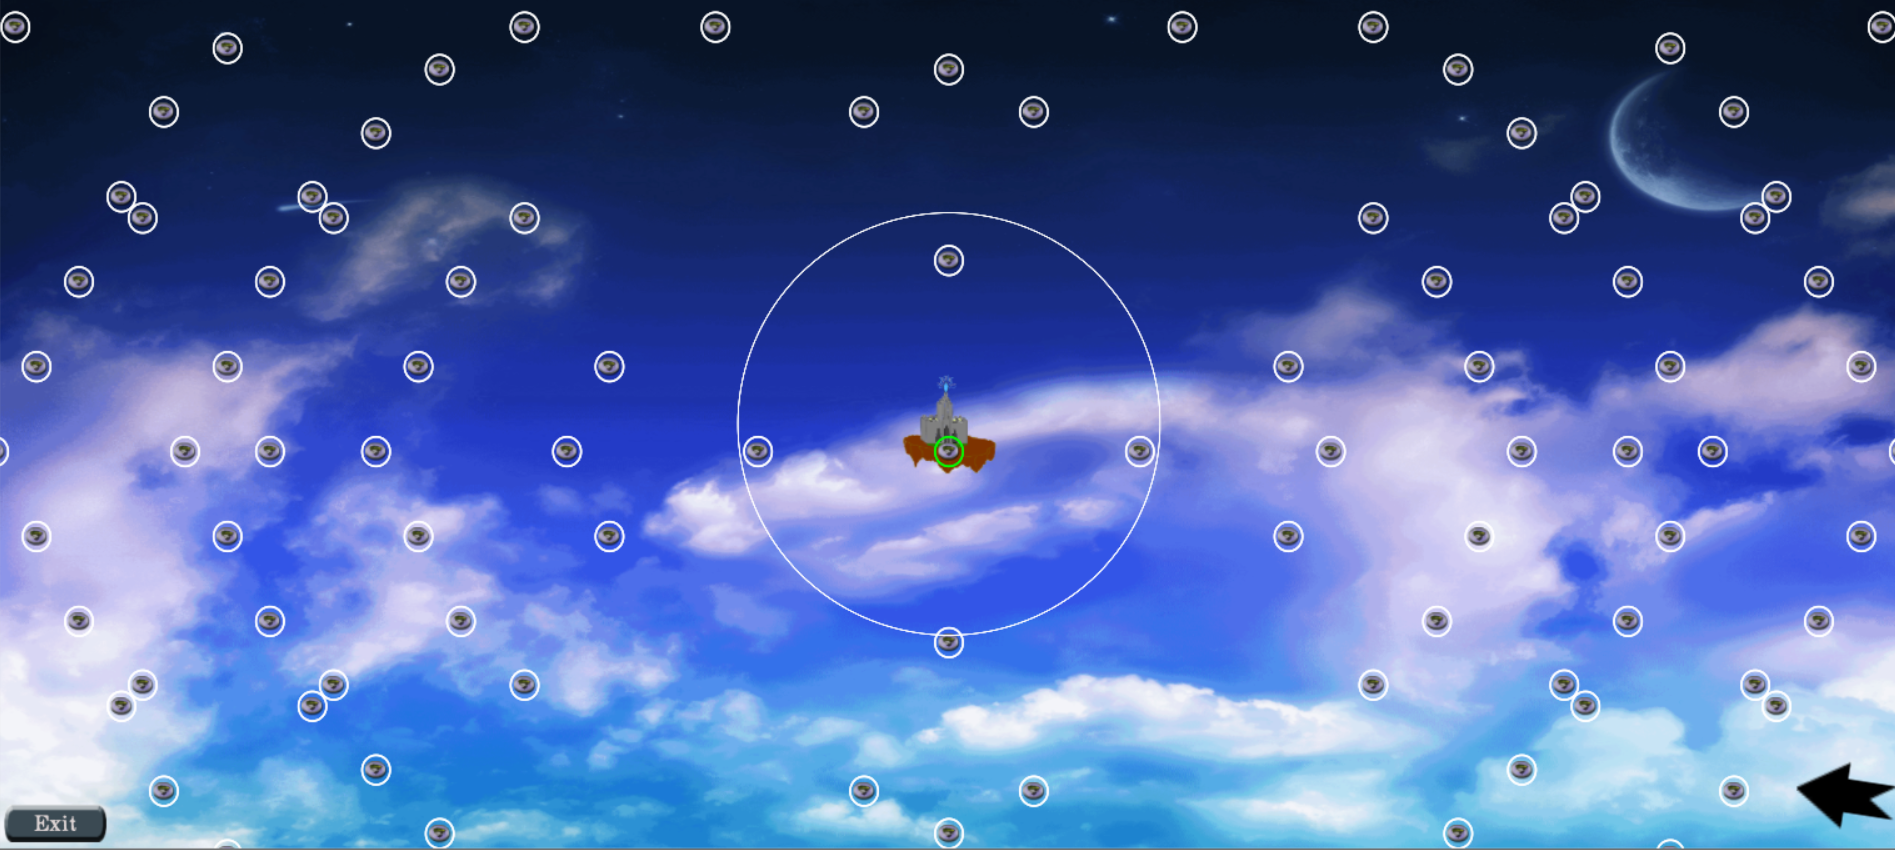
\includegraphics[width=\textwidth]{Images/WorldMapZoom.png}
    \caption{The initial state of the world map centered on teh castle, zoom out to the maximum view.}
    \label{fig:worldmapzoom}
\end{figure}

\subsubsection{Map Layout}
The layout of the map is generated by the use of an L-System (see L-system and the world map section below) and the interpretation rules that comes with it. The main map layout that is being used, has the spreading angle of 30 degrees, though this value vary from the other map layouts that were developed. The map is split up to go in 4 different directions; North, East, South and West. After each island in these directions, the directions spread in 3, one in front, and two to either side in the spreading angle specified. This is the basic pattern that by being repeated, makes up the map.

The pattern's symmetry is visible in figure \ref{fig:worldmapzoom}, where the repeated structure in each of the 4 directions is most visible in the east and west direction.

\subsubsection{Spacing}
Each of the islands that are on the map are placed in a very specific way. They are all spaced so that the distance between them are a little bit less than that of the player-castle's maximum travel distance. This is done to ensure that the players always are able to go to at least \textbf{one} island, no matter where the castle is positioned at any given time. However, because of the use of the L-System, and the fact that the placement pattern is repeating with a set spreading angle, there may be more than one possible destination at a given point in the game. Some of the islands might even be rather close to each other and look like a smaller system of islands. And of course the initial start placing of the castle has 4 islands that are available to be visited, and this is to give the players more freedom of exploration in the game.

\subsubsection{Placement}
The L-system and its rules are there to make sure that the placement of the islands are varied, but at the same time within a given pattern. This means that the look of the map will at times, depending on the how the L-System algorithm is formulated, be able to resemble specific shapes or patterns. Whether this is good or not, depends on how the players respond to it, and if they are even able to see the entirety of the map layout.

\section{PCG - Generating the content}
The purpose of this section is to shed light on the PCG used in the project, what it does and how it does so. First an introduction to the world map generation, which will be followed by the events.
The event generation will first be discussed on a structure level of the variables behind the event, followed by a dissertation of the flavour text generation.

\subsection{L-system and the world map}
\label{sec:lsys}
As described in the background section; the L-System is a way to generate a large outcome based on an axiom and rules on how to change it. With each iteration, the contents of the axiom is changed bit by bit in compliance with the rules that match each element that is being expanded upon.

In our case, we use several other characters than just 'A' and 'B', we add '[', ']', '-' and '+' as well as other letters. The brackets stand for "push" and "pop" respectively, as the map generation have to keep track of positioning, which means we have to introduce a way of saving the current state of the system.

A state as used in the generation of a map layout, has to keep track of positions and angles. So when the L-System hits a '[' in the result string, it knows that it has to save the current state at the current position, as this will be needed when the branching is done and the next ']' is hit. 

When the full expansion of the string is completed, the next stage is to interpret the result. When using this algorithm for a map layout with nodes of different properties, there is a need to use quite a few different characters. For instance, having 'N' will result in a normal node being placed at the current location of the state, whilst having 'E' will result in an end node being placed. Other characters can also be used to have different rules and calculations, e.g. having 'a' and 'A' can result in them having different angles or spacing.
Going through the resulting axiom string, we make a lot of different calculations to be able to properly place the nodes on the map. Every time a node is being placed, the direction is calculated from the state, along with the spacing. Then the algorithm moves the state's "position marker" forward in the calculated direction, and places the correct node at that mark and saves the state along with the location and angling.
This goes on until all characters of the string have been visited, and all the nodes have been placed, then the algorithm is complete.

There are many different patterns that can be made with this algorithm, and in our solution, we made a variety of them, including, but not limited to, star patterns, sea weeds, box fractals and more. 
In the end we are only showcasing the latest and biggest map pattern layout, which is a 4-way branching net of about 500 nodes or islands, that you can visit, as this is a big enough map to be able to generate a large amount of events and outcomes, and as it gives the players a large space to explore.

The map layout itself has a starting node in the center, and expands in 4 directions from there. North, south, east and west, with the initial axiom looking like this: "[N][+++N][---N][------N]". Each of these four directions are also expanding on themselves, with the main rule which is "N" $\rightarrow$ "N[-N][+N][NN]". This means that each node will spawn another to the left, right, and two in the forward direction. The angle is set to be 30 degrees, which means that there will be a good spread of the nodes all across the map. Having set the iteration number to be 3 gives us the number of nodes: 4(initial nodes) * 5(each become 5 new nodes)$\wedge$3(iteration number) + the extra start and goal node $\rightarrow$ 4*5$\wedge$3 + 2 = 502.

\subsection{Event Introduction}
In the next section, you will be introduced to the events of the game. The events are in many aspects the biggest part of the game, as the the physical part of the game, the board game part, is affected by the outcomes of the events. Furthermore the events have special requirements from the board game, and with this the connection between the 2 parts of the game is made.
In the next part of this document, we will go through the events, their structure, how they are constructed and lastly, the flavour text of the events and how they are generated and combined.

\subsection{Events}
\label{sec:eve}
The application's main purpose is to generate events which is the main interaction for the physical part of the game. The events provides resources for players and challenges in form of lost crew or constructed rooms.

Throughout the development of the game there have been several approaches to the problem of generating these events in an interesting manner and ensure the perceived space of possibilities was large enough for the events not to repeat themselves to often.

First the event structure of the final events will be explained. Then a short explanation of the first event generation, detailing where the project began and some of the limitations posed by it. This is followed by an explanation of the final event structure. Finally the how the flavour text is generated is explained.

\subsubsection{Event structure}
In figure \ref{fig:eStruc} you see the general structure of the events in the applications contextual environment. The keywords presented in this structure is referenced in the following subsections in order to specify where the different aspects are being used.

\begin{figure}[!ht]
    \centering
    \includegraphics[scale=0.5]{Images/EventStructure.png}
    \caption{The event structure layout within the application. Each event is tied to a location to on the island in the NodeScene as explained in section \ref{sec:nodeScene}.}
    \label{fig:eStruc}
\end{figure}

Each location in the NodeScene has an event assigned to it. 
Each of these events have two to three event options assigned to them. The options are represented by buttons in the UI in the NodeScene when you explore a location. An option contains the conditions required for resolving the events. 

Each of the event options contains one to three event outcome groups. An event outcome group simply is a bundle of event outcomes. It contains an outcome for each of the result types; success, failure, or neutral. These types are attributed to the outcomes.

Each of the event outcome groups contains three outcomes. An outcome has a type, as explained above, which designates which to pick given if the event is a success, failure, or neutral. The outcome also contains the chance for which this outcome appears. Lastly the outcome contains the pieces and their change amount. 

\subsubsection{Structured Events}
The first implementation focussed on having events for each of the options you could select on the UI. The events were stored in an XML file and loaded with the program. The events were assigned to all the nodes as they were generated.

The general XML structure used for the initial generation can be seen in figure \ref{fig:eGen1}.

\begin{figure}[!ht]
    \centering
    \includegraphics[scale=0.5]{Images/EventGen1.png}
    \caption{This is the first event generation xml layout. If not noted on the arrows, the relationship between the boxes is one to one.}
    \label{fig:eGen1}
\end{figure}

The events were first narrowed down by the type of the event, gathering, research, or diplomacy. The location type were generated at start along with the events. The number of events for each node where selected randomly between one and three.

Next the events were split by the button order, designated as the class, basic for the first button, second for the second button, and third for the third button. 
The classes are, basic, the one which is always present, second, events which have more requirements, and third, events which have more advanced requirements. 

In this early implementation, the conditions, which needed to be fulfilled, were written as text in the \textit{eventText} XML node. The conditions only appeared as text and had no relation to the the game logic. The text was hard coded in file, making each event text broad so it could appear in all contexts.

The event had a list of results, each which had a chance node determining how often the result would appear. When building the event the result is selected using a percentage based selection process. The chance were set between 1 and 100 percent and the total sum of all the results chances were 100. 
Each result had a flavour text associated with it, which was used when resolving the event, and a list of event outcomes. 
The outcomes represented the board pieces and the changes which occurred to them. Each of the outcomes had a piece, the board game piece associated with it, the number range of the amount of pieces given, and extra flavour, which was used for rooms which were destroyed or crew which were injured.

This first structure allowed to populate the application with events which were scripted by the type and selected from a pool of set events. 
However when adding more events, each event needed to be constructed in its entirety each time. This would also means adding or removing pieces would be have to be hard coded directly. 

\subsubsection{Constructed Events}
\label{sec:eventGeneration}
In order to construct a broader range of events, the idea were to have the building blocks to be interchangeable and then generate events from a pool of those blocks to have a greater diversity of the events.

This change were implemented through several iterations, with several changes being made to the algorithms to better suit the game. The final event structure uses an XML file containing building blocks which have a linkage to, and that influences, the general idea of the outcomes of the events.

In figure \ref{fig:eGen2} you can see the total structure of the XML file used in the final event generation algorithm. 
The events are built by selecting a number of conditions and selecting outcomes based on the selected conditions. 
First the conditions and outcomes will be discussed and then how they are combined.

\begin{figure}[!ht]
    \centering
    \includegraphics[scale=0.5]{Images/EventGen2.png}
    \caption{This is the event generation XML structure for the final event generation process. Each box represents an XML node and the writing within the name of the node. The few exceptions to this is if a name has a parentheses around it, then the name in the parentheses is an example of the node names in that level. The figure contains two parts, one for the conditions and one for the outcomes.}
    \label{fig:eGen2}
\end{figure}

The top part of the figure visualizes the structure of a condition. The condition is made up of the piece, the related board piece the players require in order to activate the event option, the amount of pieces required, and the classification type.
The classification type is used in order to group the conditions and limit which pieces appear in what event option, thus ensuring that ordinary pieces are more often in use by the application. There are 3 classification types. Type 0 for required, type 1 for secondary, and type 2 for advanced.

The bottom part of figure \ref{fig:eGen2} is representing the event outcome structure. The events are separated into types like before, gathering and research, and by classes one, two and three. 
The class in this case is the separator for where the different conditions are situated. Class one only contains outcomes which have one condition in total. It is the fall through part of the event structure as the algorithm will populate the events in the end with information.
Class two contains outcomes which have two conditions in total, and also only have events which are made up of conditions type 1 or less. 
This class is used for the secondary options available for the players.
Class three contains outcomes which primarily have two conditions, but where atleast one of these is of type 2.

The outcomes contain the the required conditions, following the rules described above. Each of the conditions have a piece, the board game relation, and the amount of pieces. 
An outcome also contains the results. This node comes in three types; success, failure, and neutral. These nodes have an attribute, denoted in figure \ref{fig:eGen2} with cursive, called chance. This is the outcome's basic chance distribution of the results. 

Each outcome has one or more options attached to it. These basically are the container for the pieces which are influenced by the outcome. If the outcome has more than one option, the one used for event resolution is selected at random. 
By having the options this way, it is possible to add more variety in the outcomes without rewriting the event in any other way.

\subsection{Flavour deconstruction}
\label{sec:flavour}
One of the biggest concerns in terms of being able to present the game with \textit{feel} to the players, was to come up with a way of generating the flavour text. The design choice made was that it would be combined by lesser blocks of text that would be combined into one complete sentence that would display the entirety of the flavour. The way to go about this, was to create dummy data and reverse engineer that into a combination system. First you would create a complete flavour text that would be served as an example. This text would contain a combination the elements that would be wanted in the actual implemented solution; Location types, island names, factions, resources, outcomes, etc.

To exemplify, we will use the dummy flavour "As you arrive at Endriath, you see an old village in the distance. The village seems to have markings that resemble those used by the Highbournes".

The next step would be to reverse engineer this dummy text into blocks of strings that could be combined to reconstruct the original text. So in the start, there is a segment that says "As you arrive at ...". This part would act as an introduction for the island. Next you have the actual name of the island, which is already available in the application. After that there is a smaller part that gives the players insight into what \textit{is} on the island. This segment, however, is split up into 3 pieces; first - "you see ", then "an old village" which is the location type, also available within the application, and lastly " in the distance". After this, the flavour goes on to say something about the location that you are currently at. "The village", again, is available from the application, "seems to have markings that resemble those used by the" - extra flavour made to build mood and a sensation of lore or story, then at the very end is the "Highbournes" which is the faction name of one of the factions saved within the application.

This way of reverse engineering a piece of text leaves us with the pieces: Introduction, Island name, Location introduction, Location type, Location exit, Location Type(again), Mood flavour and Faction name.

After all these blocks has been discovered, the next step is validation. This is done by simply making a set of paper prototypes for each of the pieces, each having a few different possibilities, and then trying to combine them in the same fashion as discovered by the reverse engineering. 

When this all succeeds, the method of combination is discovered and is ready to be implemented into code. Then, when it is all implemented, all that needs to be done is to create a variety of flavours for each of the blocks and the rest will be done by the program.
\subsection{Flavour of the Events}
\label{sec:flav}

The flavour of all the events are split up in smaller blocks that can be combined with other blocks in order to make a complete flavour string. The way they are split up varies from what type of flavour it is.
\subsubsection{The Condition Flavour}
The basic resource blocks, are based on a couple of things. Firstly, each piece has it's own intro part. This part is very basic, and is often no more that one to five words. Secondly, there is an extra block that specifies what the item/room or resource the condition requires, is. After that, there are several other blocks that are organized based upon locations. For instance, the mine will have x amount of flavour texts for each piece, just as the lake will, and all the other locations. This opens up the possibility to quickly come up with new locations, new flavours that will fit that location, and also how the individual pieces can be used there. All flavour blocks are made so that they can be combined together and form one larger and complete flavour text.
\subsubsection{The Introduction Flavour}
The introduction flavour is organized in the same manner as the condition flavour is. However, these are a bit larger pieces of strings that are supposed to give a quick and informative overview of the locations the players are entering. The strings themselves are ordered by event types, i.e. gathering or research, and underneath that, they are ordered by what specific location type it is. Each of the location types can have a multitude of flavour texts, as only one is selected at a time at any given location.
\subsubsection{The Result Flavour}
The result flavour is a bit more comprehensive than the  condition flavour, as it aiming to tell a very short story about each possible result, i.e. alchemy point gained, crew member gained, etc.
Each of these results can have as many flavour texts as wanted, only they have to be written down first. The algorithm will choose one of them for every block that is in the result. And there can be a number of blocks in a result. Yet again, each of these pieces are crafted so that they should be able to be combined with the other pieces that might also be selected, as they each specify their own specific piece.
\subsubsection{The End Flavour}
At the end of the game, there will be displayed a little piece of text telling the players that they made it to the end, and that the game is over. These blocks are not really combinable, as they are meant to be in one string alone.

\subsubsection{General Flavour}
The good thing about having all these pieces of text split up in smaller blocks of strings, is that it allows for many more ways for them to be combined. And adding more flavours will cause few problems, as they all follow the same format and template. It is basically a more structured way of generating larger combinations of text, from smaller pieces of diverse text blocks.

There are a number of different sections used to keep track of all the flavours and data that is being used within the game, and the reason for splitting them up is to better be able to keep track of where one can find what is needed at any given time, without having to go through and search through all its content blindly.
The file used for the structure of the events here is the XML file named "EventStructure". This is the main file where all the smaller blocks of text for all the board pieces, conditions and outcomes are located. It is split up into 7 branches; Conditions, ConditionFlavour, Gathering, Research, IntroFlavour, EndFlavour and ResultFlavour.

The "Conditions" is basically a list of all the possible board pieces that can occur in an event, while the "ConditionsFlavour" is all the flavour associated with those pieces.
"Gathering" and "Research" are holding the event setup, how the events can be combined, what the chances of success, neutral and failure is, and what results options there is for the combinations.
The remaining "IntroFlavour", "EndFlavour" and "ResultFlavour" are holders of the flavour of their respective fields as described above.

\subsection{Combining the flavour text}
The flavour texts are combined in a few ways. Either it is a minor combination of the location name and the owners, Which faction is fighting which faction and where, or the big ones; the conditions and results which will be discussed in more detail here.
\subsubsection{Conditions}
As the event generating algorithm has selected which conditions are to be used in the event, the flavour combination algorithm takes over. What it does, is to have the preset way of combining the flavours and then executing that template on the flavour blocks retrieved from the XML files. Let's create a scenario where there are 2 options to choose from, the first one is a single crew token that is to be sent down, and the second one is to send that crew member and use an alchemy point as well. The location of this scenario will be in a Mine controlled by Humans.
This is how the flavour text would then be combined:

In the first option, the algorithm would open up the XML file called EventStructure.xml, find the place where the condition flavour is located, and load that in. Then the algorithm would go through the branches until it came across the one called "crew". This consists of a basic text and a secondary text. The first part would be "Send", the second would be " x Castle crew". Then it would place the number of crew, in this case 1, between the 2 blocks of flavour, and end up with "Send 1x Castle crew".
Now that we have the introduction of the condition, the next step is to get the location-based flavour. The algorithm would then continue through its data until it came upon the matching location, which in this case would be "mine". Under the mine section, all the pieces are listed again, with their respective lists of flavour blocks. Say the first one is selected, which says: " to explore the mine's riches.". This would then be put at the end of the first part, and combined into the final flavour text for the first option: "Send 1x Castle crew to explore the mine's riches.".

After the first option was completed, the algorithm would see that there was one more to be done, and do the same for that, but since there is more than one piece in that option, the algorithm would do the same as it did for the crew, for the alchemy point.
An example of how the selected text would look like after completion would be this: "Send 1x Castle Crew to explore the mine's riches. Use 1x alchemy point to create a strenght potion for your crew".

On top of having the selection process brought forth from directly accessing the program saves all the previous events that has been made, and that the players have interacted with. So by having access to this information, the algorithm for the events and in turn the flavour texts of these, are able to be made by taking the existing data into account. If an event has had a special occurrence, the outcomes are saved with it and the flavour combining algorithm can then go in to this saved data, take out any important information, and use that as a baseline for the way the new event flavour is generated. Say an event happened, where the players had to use their healing powers to save a person during the exploration of an island, this information would be accessible to the app at a later time. So when the time comes to generate a new event, it can be based on said previous event. For instance; the new event would take place on an island that is controlled by the Highbourne faction, which was the same faction as the previous event, and since the players used their healer on the previous one, the new event could say that now the Highbournes are interested in knowing how the players did that. This opens up for a new set of conditions that the players can be presented with. Basic options like "Show them how it is done" or "Refuse to show them" are just 2 examples. The outcomes can then be modified to for example say that if the players were to help them out, they are rewarded with reputation gains, crystals or what ever they might get. And on the other side, the negative outcome could be something like the Highbournes tries to kill one of the players' crew in hopes that they once again will witness the amazing effects of the players' healing skills.
\subsubsection{Results}
Much in the same way that the condition flavour is combined, the result flavour is also combined. It selects a flavour string for each of the resulting rewards or penalty. To exemplify we will use the results: 2 Building materials and 1 alchemy point gained.
The combination would happen like this:

First the algorithm would go into the XML file and find the part where the building material texts are located. Then it would select one of the available flavours, for instance "Your castle crew scavenged all the possible building material they could find". This string would then be saved and the algorithm would go to the next result and find a flavour for that one as well: "As your crew return, you see that they have some strange alchemical material within their findings". 
These two strings would then be combined into one complete flavour text which would look like this: "Your castle crew scavanged all the possible building material they could find. As your crew return, you see that they have some strange alchemical material within their findings."

Should there be more than these 2 result pieces, the algorithm would go on to do the same combination and add the other blocks to the finalized result flavour.

\section{The app - From start to end}
In this section you will get an overview of how the developed application runs from start to end. 

Each of the states given in section \ref{sec:scen} and which processes that is executed and how will be detailed in the following subsections.
Each of the scenes, all have a controller related to them. This is the main component in the interaction with the visuals and the data in the app. As we go through the states, the stated actions are, unless noted other wise, directly controlled by such a controller.

\subsection{StartMenu}
The game starts in the StartMenu scene. This scene contains visually nothing but a button labelled "StartGame". 
However the behind the visuals the application is loading some of the needed data to run a game.

The Datamanager (see section \ref{sec:datman}) is loading information in the background. 
All the board piece information and all the factions, stored in xml files, are loaded and the factions are initialized. 
This data is being used throughout the entire runtime and needs to be readily available.

After all the pieces and factions are in place, the application generates the statistics of all the world nodes, their position, their description, their name, the controlling faction, and all of the statistics for the locations within it.
The only thing which is not being loaded in this instance is the events for each of the locations in the NodeScene (see section \ref{fig:nodescene}). The reason the events are not being loaded stems both from the work load and for saving computing power in the end. As it is very unlikely that the players ever visit every node and see every event, there is no reason to initialize all the events at start-up. 
All the generated nodes are stored and saved in the Datamanager so it can be used throughout the game.

The full explanation of the generation of nodes is detailed in the following section.

The scene changes once the "StartGame" button is pressed, and the "WorldScene" is loaded.

\subsubsection{Generate Nodes}
The nodes are generated when the map structure is being generated using the L-System (see section \ref{sec:lsys} above for the detailed description of how the algorithm works).

A node is generated for each of the corresponding characters in the string generated by the L-system.
The L-system provides the position of the node, along with the type of the node as determined by the character in the string. 
The node is randomly assigned a faction from the available factions stored in the Datamanager. Once the faction is set the node is assigned a name from a list of possible names, and is independently given a description of the location, which incorporates the faction set earlier.

The world node is then assigned two sub nodes which relates to the locations which will be available on the island in the NodeScene. The different nodes have an event type set, one has "gathering" and the other "research".
Each of the nodes are given a name, which is name of the location, e.g. mine; and a matching description of such a location, both based on the type of event which is tied to the node.

\subsection{World map And World Controller}
The world map in the "WorldScene" is the were the players will move from island to island over the course of the game. 

This scene starts by instantiating the world nodes based on the statistics stored in the Datamanager. As the statistics are kept in the Datamanager, whenever the players return to this scene, the same function is called, taking the changes made by the players into account. 

Once all the nodes are spawned, the controller also spawns the player object at the position which is stored in the Datamanager, initially next to the start node. 
As the player token is spawned, the main camera is centred on the token as well. As the position of the players change during the game, the centering allows the players to quickly find their bearings.

If the players enter this scene, after completing a special event, and they have managed to change their standing with one of the factions in the game, a dialogue box appears, notifying the players of the change.

As the application runs, the camera position and zoom is subject to change 

Whilst in the world map, the players has the possibility of moving the view around and zoom in and out in order to get the overview required.

Whenever an island in the world map is clicked, a dialogue box pops up which contains the name of the island along with a flavour text of the location, both acquired from the world node. 
If the players chose to travel to the location, the player token moves towards the location, ignoring any other collisions, and loads the "NodeScene" when the island and player token collides. 

\subsubsection{WorldPlayer}
The "WorldPlayer" is responsible for moving the player token as long as a target is set. 

It also controls the action to take on collision with the target island. The target of the player is allowed to be a destination which the players have already explored, however, they cannot explore it again. When a target is reached, the controller checks whether it has already been visited, and if so, the players do not load the "NodeScene" as explained above.

The last case is if the target node is the goal node. This will cause the application to load the "ScoreScene" and effectively end the game.
As the "ScoreScene" is loaded, the Datamanager is cleared of all the saved nodes, such that a new game can be started.

\subsection{NodeScene and Generating events}
Once the player has reached an island they have chosen to explore, the NodeController springs to life. 

The controller first generates the location nodes for each of the locations, as set by the L-system.
The events for each of the locations is generated by supplying the type of event and how many event options. The full description of the events is covered in section \ref{sec:eve}.
Once the event is generated, the location sprite is instantiated. Using the name of the location, the sprite related and the location of said sprite is found in a related XML file which keeps a list of all the locations, the name of their sprites, where they should be instantiated, and the scaling factor which should be used.

\subsubsection{Special Events}
\pagebreak
\chapter{\textit{Archipelago}}
The game as it is explained in the following section is the result of the design and development process explained in chapters \ref{sec:dev} and \ref{sec:tech} of this paper. Because this prototype is the one covering the largest \textit{scope} among all the prototypes created during this project, it deserves its own section of the report to be explained in details along with the analysis process of the results.
 
This playtest was performed at the end of the development and should answer all the questions raised when implementing PCG-based mechanics into hybrid games. Since the game has been thought from the beginning as an experimental concept, it is expected that the answers provided by the different prototypes will transcend the project presented in this paper. This means that the results that will be presented here will contribute to the exploration of making hybrid games in various ways: the successful design choices must be situated in their particular context, to recognize the patterns that support the hybrid nature of the gale; using the same approach, the experimentations that did not provide the expected results will also be analysed.
\section{The Final Prototype}
\label{sec:finalproto}
The first important thing to know about the final version used to playtest is that it was modified in order to cover aspects that were not working as intended. The following section will first present the rules as they were conceived; another paragraph will be dedicated to explain why these final modifications were necessary for the sake of the paper.

\subsection{The components}
Setting up the board is the beginning of every tabletop game. The board is to be placed on the surface area that the players are using, i.e. a table, and the starting conditions, like the initial resources the players have, will be distributed onto the board. Next step is to assign the \textit{Crew Member} tokens to the respective players. Each player will have their own color on their own tokens and the color itself is arbitrary: it has no relevant meaning to the game itself, rather than making it easier for the players to know which one is theirs.
When the assigning of the player tokens has been done, and the board has been placed, if the game is played by new players, the next step will be to read through the rules of the game, and to have one of the players read out loud and explain the different phases and the possible actions that can be done, along with the costs and rewards of said actions. If this is not done during the start-up of the game, it can also be done at runtime, as there is no set timer within the application, and the players can take the time they need and refer to the rules.
\subsubsection{The Board}
The following paragraph is a description of the physical board and its components. In figure \ref{fig:compo} are the board used and the tokens the players interact with.
\begin{figure}[!ht]
   \centering
   \begin{subfigure}[b]{\textwidth}
       \includegraphics[width=\textwidth]{Images/Board.png}
       \caption{The board of the final tested version of \textit{Archipelago} explained.}
       \label{fig:boardfinal}
   \end{subfigure}
   \begin{subfigure}[b]{\textwidth}
   \centering
       \includegraphics[scale=0.65]{Images/tokens.png}
       \caption{The tokens used in the final version of \textit{Archipelago}.}
       \label{fig:tokens}
   \end{subfigure}
   \caption{The analogue components used to play \textit{Archipelago}.}
   \label{fig:compo}
\end{figure}

When starting the game and placing the board, all the players have available 2 \textit{Crew Member} tokens. The \textit{Cargo Hold} contains 4 \textit{Scrap} tokens, and 1 \textit{Alchemy Point}. The castle itself will start off with 3 \textit{Crystal charges} which powers the \textit{Crystal} at level 1. In order to get to level 2, the players will need to acquire another crystal piece. Upgrading the crystal also enlarges the \textit{Cargo Hold}, which can then contain more \textit{Scrap} and \textit{Alchemy Points}.

The \textit{Construction} box is used to place the resources that were spent during the management phase, so they are separated from the \textit{Cargo Hold} - allowing for more clarity when taking decisions. The \textit{Event} box is used to remember which resources are spent during events. 

Finally, the \textit{Allies} box is used to place the \textit{Faction} card of the faction(s) allied with the players. The allied faction being an important parameter in the procedural generation of the events, it was important that players could always remember who they are allied with. 
\subsubsection{The Application}
As the application is started, the players are presented with the layout of the map. In the center is the castle, as is being represented by the physical board on the table. To move around in the world, all that needs to be done, is to click on an island that is within the ring around the castle, which indicates the travel distance possible for the castle each turn. Once an island is clicked on, a travel confirmation dialogue box will appear, and the players will have to confirm that they do indeed wish to travel there.
\subsection{Phase 1 - Castle Management}
\label{sec:p1}
Before the players have to travel around the world within the app, they have the first phase on the board. This phase is called the \textit{Management Phase}. In this phase, the players can upgrade, repair and expand their castle by building more rooms.

\begin{figure}[!ht]
    \centering
    \includegraphics[scale=0.5]{Images/rooms.png}
    \caption{The different types of rooms.}
    \label{fig:roomtype}
\end{figure}

In figure \ref{fig:roomtype} are the different types of rooms available for construction. Building a standard room (taking only one construction space) costs 2 \textit{Scrap} tokens, and 1 \textit{Crew Member} has to be assigned to the construction. This \textit{Crew Member} will not be available during the next phase of the game.
There is no limit for how much players can do during this phase, other than what the players themselves have the resources for. A room can be damaged after an event. In that case, the players flip the room and it is not usable until it is repaired for 1 \textit{Alchemy Point} and 1 \textit{Scrap} per tile occupied by the room. A destroyed room has to be rebuilt from the beginning.



During the \textit{Management Phase}, the players can also assign \textit{Crew Members} to a room that is already built. All the rooms have different effects:
\begin{labeling}{\textbf{Mechanic's Workshop}}
\item[\textbf{Mining room}] The crew members assigned to this room will gather \textit{Scrap}. The amount of \textit{Scrap} gathered per \textit{Crew Member} assigned depends on the level of the room.
\item[\textbf{Alchemy Lab}] The \textit{Alchemy Lab} is used on the board to gather \textit{Alchemy Point}. The amount of \textit{Alchemy Points} gathered per \textit{Crew Member} assigned also depends on the level of the room.
\item[\textbf{Mechanic's Workshop}] The \textit{Mechanic's Workshop} is used to repair damaged rooms. When a room is damaged, the players assign 1 \textit{Crew Member} to the mechanic's workshop to repair it. It takes one turn per tile occupied by the damaged room to repair it. Upgrading the mechanic's workshop increase the speed at which a room is repaired.
\item[\textbf{Chapel}] The \textit{Chapel} is used to heal \textit{Crew Members} that got injured during an event. It costs 1 \textit{Alchemy Point} and takes one turn to heal an injury. The number of \textit{Crew Members} that can be healed per turn depends on the size of the \textit{Chapel}.
\end{labeling}

When two rooms of the same type are built next to each other, they can be merged, thus accessing the next level and becoming more powerful (see figure \ref{fig:merge}). Upgrading a room also requires 1 \textit{Alchemy Point} per tile occupied by the upgraded room. Again, this will require a player to temporarily set a crew inactive, as it has to build the room. It is worth noticing that the crystal as to be upgraded in order to merge rooms.

\begin{figure}[!ht]
    \centering
    \includegraphics[scale=0.5]{Images/merge.png}
    \caption{The room merging system. In the top left corner of each tile, the players can see the \textit{Crystal}'s level required to build the room.} 
    \label{fig:merge}
\end{figure}
\subsubsection{Collaboration and Mastery}
The merging mechanic introduces specialization or \textit{Mastery}. In \textit{Archipelago}, all players can perform almost all the basic actions in the game. There is no specific skill related to a specific role. However, a player alone cannot perform all the actions required by the game at the same time: the amount of actions that a player can perform is directly related to the number of \textit{Crew Members} that this player commands. Therefore, it is important to encourage the players to split the tasks among them. The tasks can be divided into several groups that are related to the type of rooms that can be built in the castle. 

When a players spends one of her \textit{Crew Member} to merge a room, that player gain a \textit{Specialization token} of the same type as the room that was upgraded. There are 3 different levels per specialization, depending on the size of the room that has been upgraded after merging (see figure \ref{fig:spec}). 

\begin{figure}[!ht]
    \centering
    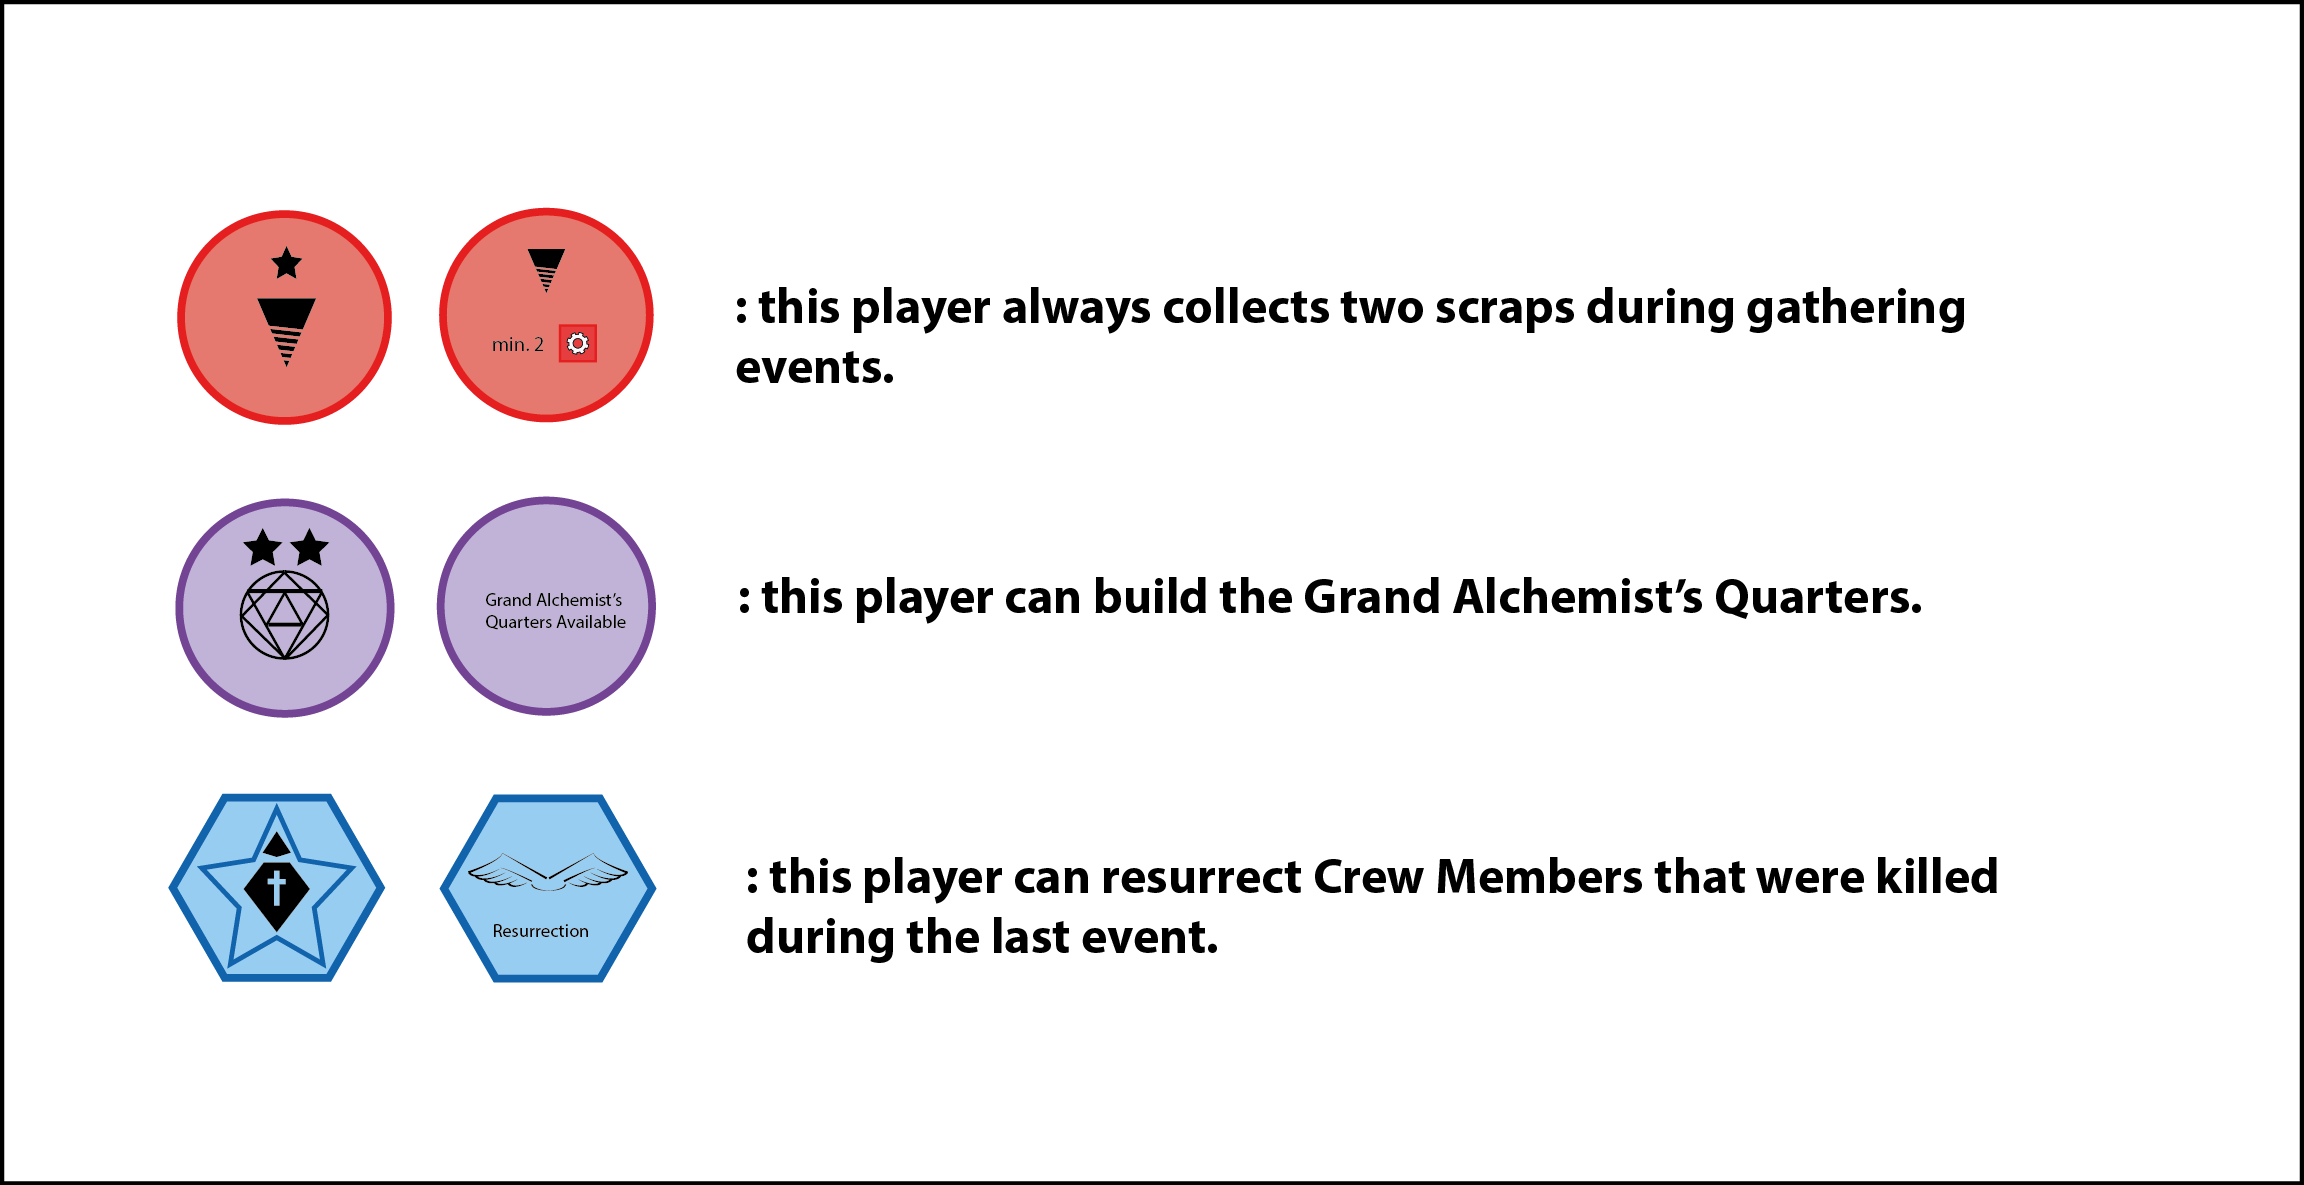
\includegraphics[width=\textwidth]{Images/Specialization.png}
    \caption{Examples of specialization tokens that players can have. Each of the tokens represents a bonus that can be useful when performing the procedurally generated events. The last token is the Priest's \textit{Mastery token}.}
    \label{fig:spec}
\end{figure}

The first type of \textit{Specialization token} grants a small bonus when visiting an island. The second type of \textit{Specialization token} always allow the player who has it to build the biggest rooms, called \textit{Mastery Rooms}. These rooms are not gained after merging. They are directly constructed for 8 \textit{Scrap} tokens, do not cost \textit{Alchemy Points} and require the castle's \textit{Crystal} to be powered at level 3. They take four construction spaces and grant the player the \textit{Mastery token} (see figure \ref{fig:temp}. This token provides important bonuses that affect the outcomes of the event.
 
\begin{figure}[!ht]
    \centering
    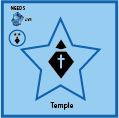
\includegraphics[scale=1]{Images/mastery.png}
    \caption{The Temple, that provides the priest's \textit{Mastery} token. The token allows the player to resurrect \textit{Crew Members} that died during an event for 1 \textit{Alchemy Point}.}
    \label{fig:temp}
\end{figure}

The bonus provided by the \textit{Mastery token} are very important, and the game can hardly be finished without them.

It is important to notice that the specialization tokens are only attributed to the first player who merges rooms of the same type. Therefore, two different players cannot have the same tokens.
\subsection{Phase 2 - Exploring the World}
\label{sec:p2}
When the first phase is over, and all the crew tokens have been assigned, the next phase is to explore the Archipelago.
As mentioned before, the first thing the players have to do in the world map, is to click on the reachable island they want to travel to. Once they have accepted to travel there, and have reached the location, the players will have to select a \textit{location} that they would like to explore.
Each area are connected to a type of resource, either it is a gathering area which will mainly yield building materials, or it is the research area which will yield mainly alchemy points. The players talk amongst themselves which one they would like to explore, and will have to choose based on what their current needs are. Once a location has been selected, the players will be presented with the event.

The player who is currently controlling the application reads out the event along with the possible options. It is now up to the players to talk amongst themselves to figure out which option they would like to pick. They also must decide which player should send a \textit{Crew Member}, according to which player is specialized. Also, the players have to remember that a \textit{Crew Member} can die in the process. The first class option is usually just sending a member of the crew down to complete the event, but there can be other options as well. The second class option adds a resource to the condition. It can be any of the four resources used in the game. The third class option requires a specialization token. In this case, it is the player that has the token that must send one of her \textit{Crew Member}. 

After the players have reached their conclusion and selected their option, the application will present them with the resulting outcomes of the event. It might be that they have lost a player token, gained one, a room has been destroyed, or simply that they got some resources. The outcomes vary. When the players have received their rewards and applied the results to the board, the players go back to the \textit{Management Phase}.

\subsection{Clean-up and start a new turn}
When returning from an event, all the pieces that were used the previous round, i.e. the crew tokens used for construction, the tokens assigned to the rooms, and the tokens used in the events, are returned to the players, and the board is cleaned up.
If an event yielded too much resources so that the cargo hold of the castle would be overfilled, it is up to the players to discuss which they would like to keep, and which to discard, before going back to phase 1 - management.
When this is done, the game repeats as described above with phase 1 and 2 and back again.

\subsection{Special Events}

Somewhere along the game, the players will most likely encounter the \textit{Special Events}. There are as of right now, two types of special events.

The first type is the fighting event. When this event occurs, the players will be presented with a scenario where two of the factions within the game, are fighting each other. It is then up to the players to decide whether they want to leave them alone, or if they would like to assist them. If they want to assist them, they have to choose their side. If the players are already friendly with one of the factions, they might want to assist that faction again. This choice is completely up to the players.

The other event type is memory based. It is an event that is based on previous events that the players have completed. The event is special in that it is based on previous data. If the players visited an island controlled by the Highbournes, and they used some special healing on one of the options, then the special event could say something like "The highbournes saw you at the island, and want to learn how to use your healing magic". It is then up to the players to decide whether or not they want to help them, or not. Keeping in mind that their current standing with the faction will influence the outcome of whatever option they choose. 

\subsection{Winning or losing}
At one specific point on the map, there is a goal island. This island is the one the arrow is pointing towards, and is the one that the players are supposed to head towards in order to complete the game, and win.
If the players are able to reach this island, the game is over. The players will be presented with an ending screen in the application, and then they can choose to start a new game if they so choose. 

There are a number of different ways to lose the game. Since it is a collaborative game, if one of the players manages to get all his or her crew tokens killed, the game is over. Every player must have at least one crew token, in order for the game to still be in play.
Should the castle run out of crystal charges, the game will be over as well, as this would mean that the castle would be stuck floating in space and not be able to move.

\section{Last Playtest}
The prototype described above is the last one that was built during this prototype. It is the result of the combination of the game mechanics created for the purpose of experimenting hybrid games and the implementation of PCG to create a new kind of play experience.
\subsection{Modifications for testing purposes}
Earlier prototypes showed that the game was not ready to provide relevant results about its experimental purpose. Therefore it was decided to alter the prototypes with a few modifications in order to obtain the necessary results. The players were not aware of the modifications.

\subsubsection{Map layout and goal}
Originally, the map should have introduced a mechanic based on \textit{interest points}. The players should not have to only reach the final island on the map to win the game, but explore the Archipelago in order to find three specific islands before going to the final island. The players are informed at the beginning that each island contains a special artefact that they need to collect and return to their king. The islands should have been possible to localise thanks to clues gained in some special events. The intermediary islands would then only be revealed when the players would be close enough (if the island is within the circle showing the range of the next move). First, the provided clues should have been visual, and thus recognizable thanks to a variety of graphical assets, which were not ready when the game needed to be tested.

It was decided to simulate it by indicating the next island to reach thanks to the arrow. The arrow only showed a general direction where the island was, and would be revealed with a halo of another colour as the one used for the other islands when the players would be close enough. This would not perfectly reproduce the intended experience, but at least it would simulate the feeling of exploration by trying to find the correct island among others. This difference between the intended experience and the one simulated by the prototype was of course taken into account when analysing the results.

When the players reach an intermediary island they are informed that an artefact has been collected by a panel appearing after solving the event.

Though in the latest version of the application, there is only one "goal" node that the arrow is pointing towards. For the purposes of having a play test that is lasting an acceptable amount of time, there were not implemented any new goals after reaching the first one. Instead the game is then considered \textit{complete}.
\subsubsection{Special events occurrences}
The special events were a difficult part of the design of the game. It was necessary to have them occurring not too often, so they would always be unpredictable for the players. This is also why they have such particular parameters to be triggered. However, internal tests performed before the final playtest with players showed that the events were not occurring often enough. 

Since analysing the reaction of the players when facing a special event, it was decided that some regular events would be pre-made and set to occur at a given turn. To do so, the island would also be set to only generate one location during this turn. Also, two out of the three options offered in the event included in that location would trigger a special event, which would ensure that the players would have to go through it before moving on to the next island. The special events were set to be triggered at least once between each intermediary islands.
\subsubsection{Progression and risk}
Since the special events are a way to increase the risk, and so the difficulty of the game, the problem of the special events not being triggered often enough generated a problem in the game's progressive difficulty. It happened that the layers would literally have very few difficulties progressing through the game, because the risk was not increasing fast enough. To solve this problem, the risk parameter was set to be also altered every time the players would reach an intermediary island.

This altered the experimental purpose of the game, because the difficulty was supposed to naturally increase with the player's progression. However, it was necessary to have more control over the difficulty so that the final prototype could offer more relevant results about the play experience itself, and not only the technical data about the generation of content.

\subsubsection{Using a portable device}
After these modifications, the application was ready to provide relevant data. However, there was a last problem that would alter the data too much to be ignored. This experiment was supposed to test hybrid games as tabletop games using a digital component to enhance its gameplay. Throughout the development of the game, the application was running on a Personal Computer during playtests. It was important for the final playtest to be able to use a smartphone or a tablet as a digital component. This would allow us to gather data of better quality about how intrusive the digital component is in the flow of hybrid games.  
Since the original development of the application had been towards a Personal Computer, the scale of all the UI elements were off when it was built to the tablet device. Everything was scaled down and was super small and the text were unreadable. This meant that the elements needed to be enlarged in order to properly supply the users with the wanted looks. At the time of the actual play test, the layout of the app was significantly enlarged, and all the elements were manually fitted to make sure that the players would experience the app in the best possible way, so that the looks of the elements would not hinder the actual gameplay experience.

\subsection{Material, Scope and resolution}
The \textbf{Material} of the prototype was closer of what players would expect when playing a hybrid game. It was the first time that the game was tested with analogue components using other material than paper, thus changing the tactility of the different pieces. With earlier prototypes using paper to iterate more quickly, the players had shown frustration when not being able to pick up the bits of paper, or losing them. Using other material than paper for the tokens would ensure that this problem would not alter the results. As explained above, the digital component was a tablet for the first time. This would help providing the necessary information related to the flow of the game. However, since the port to tablet was made in a very brief time, some problems with zooming as well as fluidity drops when moving the camera around on the map would alter the experience. This problem was explained to the players prior to testing, and taken into account in the final results.


This is the highest fidelity prototype that was created during this project. Although all the visual assets are still place-holders, the prototype uses a tablet as a digital device and that all the mechanics are implemented. 

It is the first time the \textit{faction} system and the special events are introduced in the game, and are not tested separately. Therefore, testing those mechanic is the main purpose of the prototype. By testing these two new elements and how they fit in the game, the \textit{Scope} of this prototype covers all the principles previously mentioned all along this paper. About the game itself, a progression in the difficulty must be visible when the players reach the intermediary islands. The difficulty must increase, and the decisions should be taken more carefully. Also, the players must realize that their choices have influenced the game and the generation of content. Finally, the specialization must be strong enough so that the players construct their authority in the game. 

\subsection{The Playtest}
The descriptions established in the following paragraphs are based on a transcription of notes taken during the playtest. After the game, some questions were asked to the testers. This interview was conducted in the form of an open discussion, guided by a few general questions. The observation was audio-recorded, but the playtesters did not give their authorization to join the recording in this paper. Therefore it is not included, but a transcript of the notes taken has been included as an appendix (the names of the testers have been changed).
\subsubsection{Preparation of the playtest}
The playtest has been organized in a place that all the testers know. The testers are game design students who all have  some experience with tabletop games (mostly trading card games). Two of the people chosen, had never seen the game before. They are the beginners to who the third playtester has to teach the rules. The third playtester is the only one that has experienced with a previous version of the game: if the specialization system is not strong enough, that player would take a \textit{leader}'s role - which is not wanted. The playtest will start in the normal starting conditions of the game.

The players are informed that the application is not completely ready, and that they will have troubles moving the camera around in the map screen. They are informed of the other modifications made to the prototype, except those about the special events and the difficulty progression. Those decisions were taken so that their reactions are as natural as possible when playing.

The game being a hybrid board game, the players have been informed that they could ask questions to the observers in case they could not find the solution of a problem in the rules. If the observers think that the question is legit and the answer is hard to find in the rules, they decide to give that information and take notes about how to solve the problem. 

\section{Feedback and results}

The observations taken during the playtest, as well as the open discussion with the testers showed both the successes and failures of \textit{Archipelago}. 

\pagebreak
\chapter{Discussion}
\label{sec:disc}
\section{Basic design choices} 
In this section, we will elaborate on various different design choices during the development process. How certain aspects became as they did, and the reason behind the decisions for doing it so.

\subsection{Flavour text combinations}
Early on we knew that we would have to have the flavour text and events being shown to the players. Showing it to the player required generating connected strings in some form that could relate to what was happening in game terms.
Then the question ahead was: How would this be done?
We started by having fully formed lines of text for every possible outcome and event, but realized that this was not beneficial, and that it would not create enough diversity to work as a proof of concept. 
The initial fully formed event text were rigid and would not scale well with the implementation of more pieces or with new combinations. Each time a new piece would be added, or a piece removed, would require new events to be fully written to account for the change. 

All the text strings needed to be broken down into bits and pieces that would somehow connect with each other and combine into one fully functional sentence. 
There was more than one way to approach this problem.
First way was to create smaller pieces of text, that would show their meaning, but not really combine into a well formulated sentence. This was tested out for a while, but was not the optimum solution we wanted for our product.
The next way was to generate a premade set of combinations for the events. This would mean that every possible combination that was "wanted" in the game, would have to be made ahead of time. And with every option, there would have to be rewards and outcomes for each. Again for each outcome, there would have to be at least one for "success", one for "Neutral" and one for "Enemy". With all these pieces that had to be premade, the realization was that it was sort of the right way, but that it should be the other way around. The way to go would be to generate smaller blocks of text for all outcome and option pieces, and then have extra flavour that would tie it all together. This meant a drastic reduction in how much flavour would have to be premade, and the possible combinations would be far greater. 

The "block system" solution for the text was a very efficient way to generate the combinations. It ensured that more options and content could be added to the list by simply writing in a few lines of text. If another piece was wanted in the game, all that needed to be done in order to have it fully implemented, was to write down the name of the piece, some lines of flavour for it and maybe set a chance rate on it. With these few items added, the combination algorithm is able to create a lot of content with little effort. 
We felt that this was the way to go, as having larger blocks of flavour text could probably make the sentences more nuanced, but at the same time they would be very static and stiff, and would not necessarily combine with other parts of the game well. With the solution we ended up with here, we will not have that problem, as every item is loosely connected, and by the use of connection blocks, can be combined into more rigid and well-working sentences.

\subsection{Option combinations}

There are a multitude of ways to come up with a way to combine the options the players will have. Some that were touched will be discussed here.
The first way is to have a random selection. This would mean to just have a collection of all the possible requirements that would constitute an option, and having a number of them be selected at random.
Some good things about this, is that it reduces the need for expensive and complex computing, as it only requires a simple random value to be chosen. This can of course also be influenced by a seed or a bias counter leaning towards a specific option, however then it would not be completely random either.
The fact that it is so simplistic and random, means that several things can go wrong. The same option can be selected multiple times, there may not be enough options to choose from so that the options might not be diverse enough, and the overall feel that the options are based on anything might get lost by the overwhelming randomness, just to mention some.

Another way to generate the options is to have selection based on the location. That is locations as in the types of locations i.e. a mine, forest, lake, etc. Then the question becomes what can each of the locations hold? A mine might be rich in minerals, metals and rocks, while a forest can have different plant life and a lake can have hidden treasures in its depths. These are all thoughts that needs to be figured out for this setup to work. And if this is to be the chosen method for generating the event options, how many different possibilities are needed for each location, and then how many variations of each possibility is needed? The resulting collection can quickly become very large. 
That is not necessarily a bad thing, though. Having a large base of possible options is, in this game setting, a good thing. Lots of options means lots of variety. But then comes the issue which is the flavour. To be able to present the options to the players, there needs to be a substantial amount of flavour to go with the options. If not, then having this assortment, will quickly become obsolete and bland.

Basing the condition options on the factions can be an interesting way of generating them, because it opens up the possibility of lore behind each of the factions. To take one example from our game, the "Highbournes". The highbournes are made to be like elves. High and mighty with much knowledge about the nature and stars, and generally elves have a well known story attached to them. By using known types of mythical beings, one can get a good start and overview of where to begin. By looking into already existing books and stories about these creatures, one can get ideas and inspiration to what can be implemented in the solution. Elves might have high knowledge of potions and healing, so that would mean that a possible option could be to help them out with new recipes, materials that are foreign to them, or just introduce them to "modern" technology.
However, can you cross the border between known lore and made up new lore? Does it break the feeling of familiarity?
Yes, you can, and yes it would. It would be weird if in "The Lord of the Rings" (J. R. R. Tolkien, 1937-1949) you would see an Elf using a machine gun.
But then again, who is to say that new lore and new creatures can not be made. It is just important to make it clear that this is what is happening in that case.

While on the topic of factions, another idea on how to combine the options would be to use the standing the players have with each faction. It is closely based on the factions and their lore, as described above, but when taking a relationship into account, things can get different and interesting. Using the Highbournes as example again, if the players have a good standing with them, i.e. friendly, the options might be different from what they could be if they were enemies. A friend might want to lend out some resources, have their available people assist them in tasks and quest, whilst an enemy would perhaps steal resources from them, or destroy their buildings or kill their people. The differences are immense. Taking the relationship to each faction into account opens up for a different way of telling the story of the game to the players, and it also allows for drastic changes to be made. This is something that must be considered when thinking about how the game should look and feel. In this case, the feel should be more the one of exploration of unknown islands and locations, and the creatures living there are there, not necessarily for the lore itself, but more as an extra asset that the players hopefully can relate to. The factions might have wars against themselves, and they might see you, the outsiders, roaming around with mystical potions and weird machinery. If a war or battle is going on between two factions, would the players want to assist? Or just let them be? These are all thoughts that needs to be taken into consideration when basing options on factions and the players standing with them.


Selection based on previous events
One of the nicer things when combining a board game with a digital application, is the fact that there suddenly is access to memory. And with memory, comes alternatives and opportunities. A thought that instantly comes to mind, is basing later events and options on what has previously happened in the game. One can use statistics to see which options is more likely to be chosen, and build new ones of similar sort, or one could go the complete other way, and force the players to be more diverse and have them pick between options that they have been less likely to choose in the past. Finding patterns and frequent choices can be an option and a tool in designing new options. But using this method, requires that the text and feel of the options are coherent. If they don't make sense, the feel of the game can suffer from it. So going in this direction will take a lot of thought as to how everything should be formulated in order for it to be presented in a good way to the players. A thought on how to proceed in this direction, is to have building blocks, that are somewhat loosely based on the possible standings a player can have with each faction, then making sure that each of those blocks have some sort of meaning to both the faction and the game story itself. Making sure that they can all be combined with each other and persistently keeping in mind all the conditions, would be key in this approach.

As mentioned before having saved data is a big asset to a game, board games specifically. Saving up all the data of what has previously happened makes it possible to create new content that is taking into account what has previously happened. In a game like this, one could base the next options and outcomes on what the players have gotten during the events and actions leading up this far. If the players have been taking the easy option all the way, maybe it is time to challenge them and take away the possibility for an easy action. Maybe all the outcomes they have gotten so far has been negative? Having access to the saved data, and also \textit{when} the results occurred, can be a valuable asset, as it gives the opportunity to change the entire course of the game. It makes it possible to have adaptive difficulties, and one can also give the players the option to select and change difficulty on the go. Combining the options based on the previous results, can be tricky, however, if the options and the results do need to be directly linked to what has happened before, one has to take into account that it is not only the values that are presented to the players, but also the flavour texts. And the flavour text is what allows the players to become part of the \textit{world} that is the setting in the game itself. If there are major incoherences, the feeling of a polished experience can easily be broken. If going for this way of generating content, this fact must be in the back of the head. It can definitely be used as a way of generating the content, but there might need to be a secondary check whether or not the wording of the options and results are working and fitting. Grammars and the ordering of the words will be an important aspect when combining the generated contents into a finalized product.

Earlier there was a mention of changing the difficulty in the middle of the game. Another way of making the options, would be to do this difficulty change gradually as the players progress. Starting off easy, and then getting harder and harder. Or the other way around, easier and easier, if that is preferable. If this is what is wanted, there has to be some sort of scale that shows what constitutes hard, medium and easy. When this is established, the algorithms can be made into generating the content on a declining or increasing scale. How much is going to be changed, and how much it will be modified each turn, is then up to the scaling system itself, or the players, if they are given the possibility to set this themselves.

While on the topic of gradually changing the content, another way that comes up, is to increase the costs and rewards based on stages.
Each stage could be a finite amount of turns, or a stage can change to the next one when a certain threshold has been reached, be it turns, resources gained, resources lost, etc.


The ways described above are singular ways of generating the options, however in a complete solution of the problem, one might want to combine two or more of these ways. 
We are using a combination of basing the options based on the location, as well as factions. Some of the events, i.e. the special events, are based on location, factions and standing. They get all this information from the previous events that has occurred, and by utilizing the memory of the application, it is able to give the players a \textit{shock factor} that would not be possible with a traditional board game. Containing the information that has happened before, opens up the possibility to startle the players with new content based on previous events. 
By mixing in an element of randomness into the mixture, it is possible to change the entire feel of an event, as the values might be slightly out of context, but still enough in context that it can be made sense of. All these mixtures is what makes it possible for multiple ways of handling the events. And by creating the options for each event as soon as the players enter them, it is possible to create varied outcomes as well. Each option can have an outcome based on how it is formulated, and by having this, the events can become very different and the range of which they impact the players is potentially increased. 
If the events are gradually changing, then the memory part can be a big influence. It allows the application to \textit{know} where in a game session it is, and from there, it can utilize different algorithms to change the difficulty, range of options and impact on the outcomes, that each event has. This can create a feeling of progression for the players, and make the feel of the game more consistent and make it feel like the game has more of a purpose to it.

\subsection{Layout of the map}
During development of the application, there was a discussion whether to use a pcg-algorithm in order to create the map, or to manually create it and have it saved. The conclusion was to use the L-System in order to be able to quickly generate maps, as having more than one map would give the players more replayability and diversity, and by using an L-System there was the possibility to mutate the rules of generation, and have a constantly changing layout. By changing the values such as the spreading angle of the island placement, the map would be different in looks, and by changing the number of iterations of expansion of the axiom, the map would become bigger or smaller. Then by introducing a random value for the angle and distancing of the islands, the maps could have a layout that would never look the same, and that would have a variation of turns and angles and distances from one island to another. However, by doing this, the calculation time for the L-System could become very large, and that could also ruin the player's interest for the game. So by compromising and rather create a multitude of different pre-set patterns, the execution time can easily be managed to be within the time frame that is required, and it allows for more controlled diversity within the layouts of the map.\\

A rather substantial problem with the L-System, is that it can become very large, very fast. This means that it can reduce the quality of the application, and consume too much of the resources of the device the application is running on. If the system is too big, and taking up too much resources, it can potentially freeze the system, and overheat the device. This is of course not a preferred scenario, and so it is better to have a controlled environment where construction of the rules and axioms of the different layouts to be produced by the system can be monitored and managed.\\

Our solution has a total of seven different and diverse map layouts, that are available within the code, however, for the sake of managing and testing the game and making sure the produced results and gameplay is coherent, only one of them will be used. This decision was made, because the need for some continuity was needed in order to make sure that all the aspects of the game; the flow, the board, the events, user interaction, etc. all were working as they should. 
Some of the other maps were smaller, with fewer possible destinations and events, and so they could be suited for a tutorial if that is desired. But for a full game, the need for a bigger map layout with all the islands in a set location is outweighing the need for diversity and changeable maps.


\subsection{Board layout}
During the development of Archipelago, the layout out the board changed many times. The original layout consisted of a partitioned grid of boxes, wherein the rooms would be placed. The partitioning were made so that each part had a different color that indicated the tier level of the castle. Each tier would require a certain amount of crystals in order to be functional. 
As the development process progressed, the layout changed. With each prototype came a new layout, and additional feature were added. These features were cargo rooms for storing of the players' resources, a crystal bar for keeping track of the crystal tokens, an event box for when the players would send out crew tokens on events, and a building box and for putting crew and resource tokens in when managing the castle and building new rooms or upgrading existing ones. 
\subsection{Tokens and rooms}
Archipelago has a multitude of tokens and rooms, and over all iterations of the development process, they have been redesigned, added or removed from the game. Each token that would be in the game had to have some sort of functionality and purpose, otherwise they would be rendered useless and feel like more of a nuisance than a contribution to the game. One aspect that ended up being completely removed from the game, was the diplomacy room and specialization tokens. Originally there were meant to be three types of event types; Gathering, Research and Diplomacy. However as the development of the game continued, and with feedback from playtests, the Diplomacy events ended up being scratched. It did not get the desired results that were wanted, and it did not give the experience we wanted for the game. Instead of having a diplomacy aspect to the game, the events would instead have diplomacy implemented through the use of special events and a faction system. This made the game more fluent and gave the game a better feel of being polished, as the faction system would both add to the story and setting of the game, as well as giving the feel of conflict in the game with each faction being against each other, and the players having to choose their sides in these conflicts either directly through special fighting events, or more indirectly through memory based special events.

\subsection{Story}
In the start, there was not much story or concept of story, since it took a while before settling on a theme for the game. However, as we came up with different ideas for different themes, a part of the development was to have some sort of story basis in the back of our heads that would combine with the overall theme. Since we had the concept of a node-based system, every story and theme we would come up with, would have to support this. The world would be made up of a large overview of the map that had smaller "nodes" that the players would be able to visit. Each one of these nodes would then have smaller nodes within them. 
With a theme of pirates, the story would become something along the lines of the pirates would travel on the oceans from island to island, from port to port, and there they would be plundering all the villages and taverns they could find. In this case, each outer node would have smaller areas within it that would be the different places the island would have, like a tavern, village or other types of hubs. We were also considering the concept of space. Having a spaceship that would travel through the universe, visiting planet after planet, and exploring the areas of each one of these. Since the whole space scenario is a rather big one, and the science-fiction stories are many, coming up with an original and consistent story for the game, would be a rather immense task, and the risk of it being too generic or on the other side, too abstract, was something that had to be kept in mind. 
In the end, we landed with a more fantasy theme, with a floating castle that would travel around an unknown world where other people and factions would roam the lands and fight amongst each other. The story behind this scenario is that you, the player, are in control of this large floating castle, that is lost in a new and unexplored world. It is up to you to make sure that your castle and its crew are able to get to the destination safely. You will have to explore the vast world and its islands that are scattered around in all directions and expand upon your castle and try to power it up by getting more crystals like the ones that are powering up your castle. Along the way, you will encounter new races and factions, and see vast forests, huge lakes, old villages and factories, and it is up to you and your crew to gather what you can from these places and rebuild your castle and get home safely. You will make new allies and enemies along the way, so be careful not to aggravate the people you meet, or they might just attack your crew or your castle. Manage the castle efficiently, or you might just get stuck, floating in mid air in an unknown world, never to be able to return home.

\subsection{Theme}
There was a lot of different themes going around during construction of the project. The initial thought was Space and something in the lines of FTL: Faster Than Light. 
Other themes that came up were "Western Caravan" in a sort of "Mad Max" setting, "Pirates at sea" travelling from islands to islands, and plundering what they could find, "Magical Flying Castle" that would fly through a vast world of floating islands with unexplored areas of varying types and locations.
The last one was chosen. The reason for this choice, is that it gives us a feeling of familiarity, as it is in a fantasy setting, and most people are familiar with some sort of fantasy story, whether it is "The Lord of the Rings", "The Chronicles of Narnia" or other fantasy stories. Most games that are in this genre and has creatures or factions, usually have a connected base that is the basis for all fantasy. Usually it contains Orcs, Elves, Dwarves, etc. and this makes it easier for players to accept how the feel of the overall game story is set. 
Going with the theme of a flying castle roaming the skies, the setting itself would be some combination of the dark ages mixed with fantasy. When you see a stone castle, you usually think of the dark ages, and when that castle is flying, the thoughts go to a more made up world, a fantasy world. 
Having this fantasy aspect in the theme, allows there to be almost any types of creatures and areas, as they can be created from scratch and added into the story, as fantasy have room for any new things that might be created.

\subsection{Gameplay}
\subsection{Connection between Board and App}


\section{Collaborative game} 
Archipelago is after all a collaborative hybrid game. And this came through during the playtests. When people played the game for the first time, there were of course some minor confusions as to how the game was played, but after getting into it, they showed more and more interest in taking charge and communicating between the players. At one point there was a player who made a new meta game within, that she wanted to be the first of all the players to have a tier 3 room and be the "master" of that room. It is interesting to see which player behaviours are appearing when playing the game. And this case was rather pleasing, as it introduced a competitive element in the game, that was not intentionally placed there, and although it did not necessarily have any real impact on the game itself, it certainly had an impact on how the players enjoyed and played the game amongst themselves.
\section{The 2 phases of the game}

As described in the Final Prototype section (see \ref{sec:finalproto}), there are 2 main phases of the game; the management phase (see \ref{sec:p1}) and the exploration phase (see \ref{sec:p2}).\\When in the management phase, we noticed that some times the phase could end rather quickly. This usually came as a direct result of the players not having enough resources to do anything useful. Either they had to save up more resources, or they wanted to save them in order to possibly spend them during the events in case they were needed. This is of course a mechanic within the game, as this is a management kind of game (see \ref{sec:management}). It was rather interesting to see how the players would adapt to sudden changes and events that took place within the game, and how their tactics changed when the completed events yielded a penalty instead of a reward. Suddenly a room needed to be repaired, and that meant that they had to build the room that allows for that mechanic to happen, the mechanic's workshop.

The second phase, the exploration phase also proved to have varied behaviour of the players. During the initial first explorations, the new players were uncertain on which option to select, partly because they were new players, but also as they did not properly know the risks that comes with the different options. However as the players became more and more comfortable with the game and the rules, they started to become more determined, and sometimes took a more "aggressive" or "reckless" approach. Instantly wanting to take the more costly options, sometimes even without thinking about whether or not the controlling faction of the island were hostile. This meant that the outcomes had a greater chance of being negative, and when this happened to the players, frustration arose. 

It is good to see how the players change their attitude once something bad happens, like when they were penalized from an event, we could instantly see that they had to re-evaluate their moves in the upcoming rounds. 

Seeing that the players would change their tactics during the course of a game makes the game feel rather successful, as it made the players talk more amongst themselves, and it made for varied gameplay.

\section{A management-game}
\label{sec:management}
Although having elements of both exploration and strategy, the game itself is a management type game. What the game of Archipelago focuses most on, is managing the castle as you explore the wider world. Having this as the main mechanic of the games encourages the players to communicate and collaborate to make sure they are able to reach the winning conditions of the game. The game encourages the players to upgrade their castle and build rooms and upgrade them. But in order to be able to do so, they must gather the resources needed. This is done by completing events, and even there, the players have to manage who should send their player tokens out on the mission, and which missions they should complete in order to get the resources they need. Since the players have to manage their resources, and more importantly for the win - their player tokens, discussion and tactical thinking is being enforced onto the players. One player might want to take charge and be the "brains" behind the team, and that is O.K. because any player behaviour that causes the players to be social and interact amongst themselves is valuable for the game. We want the players of Archipelago to get into tactical discussions about how to manage their castle, what to build, what to upgrade, and we want them to be able to think ahead in the game and come to agreement on which events to pursue. 
\section{The result of the game}
As the development period is over, there are a number of things that can be said about the game that was created. Since the finished product is not meant to be a completely finished and polished game, the visual looks of it was not the most important aspect. The board itself is just printed on a piece of paper, and the tokens are made of cardboard. This would of course have been different if we had planned to make a more visually pleasing game. If this was the case, the board would have been made of proper hardboard materials, and the tokens might have been the same, maybe even some would have been in hard plastic. When it comes to the application, the same goes in terms of looks. We did not put too much pressure into the graphics of it, and there are still a few bugs here and there. This is all inevitable as the development period is only around 5-6 months. Looking over the code after having completed the deadline for developing, we find a lot of things that could have been done different e.g. duplicate code, redundant calls, etc. Again, this is to be expected, and these are all aspects that can be fixed and modified during future work.
When it comes to the algorithms used for PCG, we are pretty happy with them, as they do convey the concept of introducing PCG and its benefits in analogue games and hybrid games. The way we generate the events and the flavour of them proves that having a digital aspect in a game can be beneficial, and that it removes the need for having lots of cards and extra rules. 

\section{PCG contribution and its benefits}
\label{sec:pcgben}
What the PCG part did for this project, was to remove the need for the physical part of the game to have cards, map-board, a pre-written explanation on how to set up the map locations, and it removed the need for dice rolls. This being a collaborative game, the focus of the players needed to be more on each other and the \textit{story} of the game, rather than having to focus on reading from a piece of paper each turn, each time one rolls a die, and each time a card would be picked and had to be combined.

One of the biggest ways that PCG has contributed to the game, is to have given the game access to memory. This means that the game can suddenly surprise the players by presenting a newly generated event that is based on occurrences that happened maybe 15 turns ago. Unless the players have a book to write down every little detail of the story as the game unfolds, this would not be a very likely scenario to carry out, without the use of PCG. 
Having memory also opens up for the possibility of hiding information from players. Take the faction system for example: most of the information is hidden, and the only thing the players see is the little dialogue box that pops up when a faction's allegiance has been changed from one to another. This means that the only information the players have available is their current standing with the factions, and they will have to remember it themselves, as there is currently no way to see the current standing with any given faction, except for when said faction standing is changed. If the digital aspect of the game was not there, then the players would have to take note on the standing with each faction, and whenever a faction specific event would happen, they would have to use a different combination method for the events and the flavour, and maybe even have a separate deck of cards, which would mean more to keep track of, and more to carry around and set up in the game.
As for the events, the way PCG contributes, is to allow for quick gathering of information about the event details. The algorithm used generates varied results every time, and gives the game an expansion possibility that would not be the same if the events were selected from a pre-made static deck of event-cards. In order to expand upon the game and make it bigger and better, all that is needed, is to add more types of locations, factions, Options and outcomes, and flavour blocks for each of these into the XML file that contains all the information about the game, and then it would be like having a 500 piece deck of card added to the game.\\
When it comes to the map, the layout possibilities that PCG enables, are endless. Right now the system uses an L-System to generate the layout and place the islands at their correct locations. This is quick and efficient, and allows for endless ways to set up the map. By adding more rules, and specific interpretation logic for them, into the system, each new map can be made to have different experiences to them. You could maybe make a map that looks like the actual world? 
On top of just changing the map's layout, you can add quests and puzzles into the map itself. If combining the L-System with graph grammars, the map can be made so that one island has a quest assigned to it, and that quest could for instance have the players move towards another side of the map, to one specific island. The end island could then be hidden from the players completely, and only be showed/enabled when the players had reached a certain part of the quest line.

If the map was to be analogue and have all these possibilities, the physical weight of the game would potentially be enormous. Either all the map layouts would have to be able to be made with one set of pieces, or each layout would have to be made individually with their own pieces. And if there would be quests and quest-lines assigned to the maps, the rules for how they were played out would have to be thought out in advance, and they would probably make for a very \textit{similar} gameplay each time the game is played. PCG, however, enables the game to have varied contents every time.

By utilizing the memory of the application, the events and the content within them can be changed every time. It also makes it possible to have a difficulty curve within the game. By saving resources gained and lost on the events, the following events can use this information and take it into account when generating new ones. If the players have not received enough of one resource, the application can catch that, as it is saved in the memory, and then it can take countermeasures to make sure the game is able to progress. This would not be possible without the memory, and if the game was purely analogue, the players would either have to cheat and take extra resources without it being in the mechanics, or they could potentially lose the game, or have to start over. Of course, had this been a purely analogue game, the mechanics would have been made differently to account for things like this, but as it is not, the memory of the application serves as a valuable tool both for the game in its current state, and for possible future work on it.


\section{App vs. boardgame design challenges}

- Which elements should be in the app vs which should be on the board\\\\
- Representation of the castle on the board from looks on screen\\\\
- Pieces needed within the application, taken from the board\\\\
When coming up with the mechanics and the pieces needed in the game, we also needed to figure out which pieces and elements should be in the application part. Since the story of the game required "people" to explore the islands in the world, and complete events on them, there was a need for the app to have player tokens as an input. Same goes for the resources that are used in the game. If an event required building material as a condition for the resolution, this would also have to be stored in some way in the app. One could argue that instead of having these parameters in the app, the algorithm behind the events could just generate several different and randomly connected outcomes. However since we want to explore the PCG aspect in connection with hybrid games, it is better to make sure that the application has the correct inputs and values so that it can generate content that actually influences the players' behaviour, and that is influenced by it.\\\\
- One aspect of the game should not overpower the other (The app and the board should be "equal")\\\\
The balance between the physical and digital part of the game as a whole needed to be kept intact. The word "hybrid game" itself would be rendered rather redundant if one of the parties would take over the players completely. If they are constantly looking at the board and neglecting the app, is there even a purpose for the app. The same goes for the board and if the players are constantly looking at the app, and not paying attention to the board. There needs to be a balance between the two. Either let the flow go from one to the other and then back in repetition, or have both aspects be equally important at any time in the game. Archipelago utilizes the first method, as the game consists of 2 phases. And in our game, the physical part is dependent on the app in order to give any purpose, while at the same time the app would be pointless without the board and the pieces to enable proper play.\\\\
- Removing cards from the game, and introducing them as PCG\\\\
Whilst designing and programming the game and all the functionalities of the app, it was decided that there would not be any traditional cards in the game. At least not in the physical part of it. Instead we would have a way of introducing the "cards" in the application part. This decision was made to enhance the purpose of the initial problem statement proposal, that we want to explore the PCG aspect in hybrid games. Making the cards, or at least the text that would be on them, via the use of PCG algorithms would make for greater variation, and would give more purpose to the application part of the game.\\\\
- The story and theme\\\\
- Graphics and visual representations\\\\
Since the theme of the game ended up on being a fantasy based dark-ages one, we wanted the look and feel of the UI to be somewhat rustic and stony. We ended up with making our own graphics for them. The background of the dialogue boxes and the buttons, even the player castle. We could possibly have found pre-made graphics online, but as they might be copyright protected, we came to the conclusion that it would be better to take a little extra time and do it ourselves. Since the main concept of our problem statement does not necessarily concern the graphics all that much, the creation of these graphics were not a big concern of ours, and was held off with until late in the project. It was more important to focus on game design and PCG implementation, and the fact that neither of the members within this project are graphical designers only enhanced this decision.\\\\


\section{Benefits of having memory in the app}
As described in section \ref{sec:pcgben}, having memory in the app is a big benefit to the game in total.
It opens up the possibility of having ever-changing events and content within the game, as the newly generated content can be based on previous content that has been saved into the memory of the app.
It allows the game to have player control in terms of the resources given to the players, along with possible negative effects to the players; penalties. The memory can influence the PCG algorithms in ways that would otherwise have to be done manually, e.g. if at the end of a turn, the players would have to type in how many resources they have of each type, and what they have spent, etc.
Since there is now memory in the application, calculations can be made to see which types of options the players select during an event. For instance, if one event has a third option that requires the players to have a specialization in healing, the application would then be able to calculate that the players have used at least 4 building materials, along with 2 alchemy points in order to get that room. The application would then do the calculations and save the result in the app, that the players now have 4 less materials, and 2 less alchemy points. Without the memory, this would not be possible, and the application would rather have to have set rules for how the events could be made up, or the players would have to give the app inputs so that it would know where to continue.
So one of the biggest benefits with having memory in the app, is that it allows for continuous generation of content that is directly connected to preceding events and content, and the current state of the players' resources.

\section{Possible alternatives to our solution}
One of the most obvious alternatives to our solution, is to create a complete board game, or a complete digital game, instead of using both as a hybrid. However this would not be in the scope of the project, as we want to explore the space between PCG and Boardgames by the use of an application and the making of a hybrid game.
As briefly mentioned earlier, it would be nice to take more use of the map, its layout and its possibilities. Creating quest lines and hidden events that would occur as the game progress. What would also be nice, is to have a route within the map, so that the players do not necessarily have to just go towards one node, but have one node at the start that is the first goal, then having other goals afterwards as they move through the map. 

\section{Team Dynamics}
Since the project group consisted of three members, one designer and two programmers, it was only natural that there would be a more intimate collaboration between the two programmers. We would all sit in the same closed off area and work, so that we would always be able to communicate issues and ideas, and give feedback to each other when needed. The programmers would usually work either side by side, or opposite of each other, and work on their specific tasks. Whenever problems or issues occurred, they would be able to simply look at the other person's screen and help with feedback or code review. The developer would also work closely with the programmers, as all the code that was being written had to originate from the concepts that the designer would come up with. During the brainstorming phase all parties would work together in order to come up with joint conclusions and ideas as to how the game would work. The designer communicated the ideas and needs for the project well, along with new updates and functionalities that would have to be implemented into the application in order to make the digital and the physical parts of the game come together and work as one whole game. 

Whenever a person was sick, or had personal errands that made it impossible to meet up in person, we would use the Slack \cite{prog:slack} communications program in order to stay up to date and in touch. Also by having access to Trello \cite{prog:trello}, we could plan all the tasks that needed to be done, and have an iterative development method, scrum, that we would follow. These programs were essential to the development process, as it allowed all the members of the group to easily be able to have a quick overview over all the tasks that needed to be done, and it made it possible to add new tasks as they arose, with everyone being able to get notified when that happened.

\section{Issues}
During the course of development, we did not have direct access to an android device for testing. This meant that as we developed and tested the application, we had to do so by the use of laptop computers. When we eventually got access to an android tablet, there was a rather substantial problem with the scale of the UI elements. The text was to small, and the dialogue boxes were not based on the resolution of the tablet's screen. So for the sake of actually being able to do proper play tests with the app in a portable device, we would have to manually go into the code and scale all the elements so that they would fit the screen of the device. A different approach that could have been taken, in hindsight, is to have used relative dimensions and made the scaling adaptive to the screen the application would be played on. However using the Unity3D game engine, all the elements are set to be a pixel based size by default. The UI elements are put into a canvas that acts as the place holder for all the child-elements. This canvas is then directly based on the size of the camera view frustum which when used by a mobile device or tablet, scales down pretty significantly. 
Another issue that was discovered by playing \textit{XCOM: The Board Game} \cite{game:xcomtbg} was that when playing a hybrid game, and using a mobile device to handle the digital part, if the program is too resource demanding it will drain the battery of the device. When we played this game, this happened to us. Fortunately we had a charger available, but not before the tablet shutting down completely. The good thing about the app for this game, was that it saved the progress as you went along, and was able to resume the game from where we left off when restarted.





\pagebreak
\chapter{Conclusion}


The creation of \textit{Archipelago} had the purpose of exploring a new type of tabletop games using digital components to enhance their gameplay. This was done thanks to the use of PCG. This chapter will conclude the project by answering the questions at its origin. This will be done by identifying the key results of the experiment based on the constructed framework and on the knowledge gained thanks to the playtests, and the development itself. Finally, the last section will show how \textit{Archipelago} paves the way for experimentations relative to the purpose of this project.

\section{The exploration of hybrid games}
Introducing PCG to hybrid games created a much bigger perceived possibility space regarding the game's content. Compared to regular hybrid games, where there is no specific PCG involved, \textit{Archipelago}'s algorithms and structure allows for more content to be created while at the same time enabling the possibility for there to be pre-made content. 

Through the work done with developing \textit{Archipelago} as a hybrid game, many challenges relative to the ordinary approaches of board game design were discovered. Creating such a game within an only slightly investigated field actually proved itself to be a challenge. When developing both a physical and a digital game concurrently, one of the most important factors is that the mechanics design is thought through and that both the board game and the application have equal, yet distinctly specific purposes. \textit{Archipelago} is different than already existing hybrid games such as the ones described in this paper. The first aspect underlining this difference is the fact that \textit{Archipelago} does not require inputs from the players solely in the purpose of directly feeding the application with information. This was an important mindset to keep during the development of the game in order to preserve the tabletop experience and use the digital device in a smart way, to avoid the use of such inputs.

Another principle on which \textit{Archipelago} was based on was to make the game entirely dependant on the digital device that is used to support its mechanics. This was achieved by basing an entire phase of the game on the use of the digital device and its computing powers. By creating mechanics that require both types of components and making the game collaborative, the game illustrates this approach of hybrid games without denaturing the traditional tabletop game play experience.

\subsection{Increased replayability and adaptability}
When developing \textit{Archipelago} and by utilizing PCG in the hybrid game setting, we discovered more uses and ways to take advantage of the processing power that a digital device holds. Our main focus point in the game when it comes to PCG, was the events and the flavour associated to them. Developing and when reflecting on the process showed in what ways PCG could be useful. Having the algorithm for the events that is used by \textit{Archipelago} allows us to simply add more information into the system and be able to get new content in a way that would not be possible with only an analogue version of the game. If we add more pieces to the system, and then bits and flavour that match them, the system is able to generate a completely new content, that could be seen as a traditional expansion set to the game without having to physically take up more space and time. The power of the PCG algorithm is that it allows for the continued generation of new content with minimal effort. By using PCG combined with the L-System, the game affords the players to have a vast area to explore in any direction. New rewards and penalties can be added as the designer sees fit for the game, and once these rather small pieces of information are added to the XML file, everything can be implemented automatically. The events are the place where the application delivers content to the board game which is hard and cumbersome to replicate using only analogue components. The multitude of events and the different combinations which can be achieved would require an immense set of cards in order to be comparable. 
The special events, which uses the players previous actions, are even harder to replicate. The cards would have to have some sort of combination mechanic based on visited locations and which factions they have interacted with and how that interaction has been conducted. They also illustrate how PCG should be used to make the players feel that their actions have an influence over the game's content.

\section{Future work}
\label{sec:future}
In this part, we will elaborate upon possible work that could be done in the future. This includes what we would like to implement, thoughts on how to do it, and what could have been done differently in order to make this easier in the future.

\subsection{Better use of saved data}
\label{sec:savdat}
One of the big impacts this project brought to light, was the use of saved events and its data to generate new events that were based on those. In this solution, we save the events that happen over the course of the game, and we use them in a rather minimalistic way, more as a proof of concept. However, it would be interesting to see how this data could be used more efficiently over an entire game session. Generating more experience driven content, that would have a bigger impact on the players' experience, by creating other mechanics in the game, is one thought that comes to mind. 

The saved data could be used in ways which a board game could never compete. One could use the saved data to challenge the players either more or less, by knowing the number of resources they have collected, and tailoring the possibilities from that knowledge. In this way, the game would either challenge the players to use their resources wisely or give them access to a resource which has been sparse in the previous events. 

The special events could really play to what the players had been doing, in terms of where and for who, giving the players a greater feel of involvement in the world. This could be shown with some sort of faction overlay, which could change each time you dealt with the different factions. It could be possible to have some sort of background faction warfare with variables being influenced by how the players interact with the game.

Also, a story could be brewed by linking all the outcomes of the events. In the end building a short story based on the players events. Using a text algorithm of sorts to create a story based on the factions relationships and the deals made at each point of interest. 

By using the current layout, one could even imagine that the application could piece together the state of the board game, using the input from the events. Whenever the players resolve the events, they declare, indirectly the tells the application how they have used their resources. Saving this could help to give a complete look at how the players are doing and surprise the players by revealing to them in events that the application knows what they have built.

In the end, the saved data could be used in many ways to give the players a feeling of a game which reacts to their input, even without them having directly to manipulate the application with the results and state of their board.

\subsection{More options and outcomes}
At this point in time, there are a finite number of possible outcome types, rewards, and penalties. For a future version of the game, it would be interesting to see how the game would be experienced if there were more types of tokens to be played around with. It would also be nice to have more flavour text pieces that could be combined, maybe in a new way, and presented to the players. 

Right now the system is capable of combining the different parts of the game and generate events with flavour text, using a combination of the board pieces and flavour text strings.
The system is built such that more pieces could be added, along with flavour text bits for each of them, and still generate meaningful events. 

However, there is right now around 3-7 text strings for each of the board pieces, all of which can be combined which each other. This could, of course, be increased, but it would also be interesting to generate text which is capable of having some sort of interrelation between the pieces. 
This could perhaps be accomplished using some sort of grammar such as the L-systems, which could take the current text being built and use it to create a better interrelation. 
The grammar could as an example relate Alchemy points to Castle crew and base the flavour text on some sort of potions to improve the crew, or relate the alchemical potency to how it improves the machinery used in a specific event. 
Having this relation brings the game more to life and makes the players feel more immersed in the experience.

In the end, having more pieces, a variety of flavour, and ways of combining the flavour, would be like creating an expansion pack of cards that would be added to the physical board game.

\subsection{Additional features based on the map}
The current map layout generates a larger structure of floating islands which you can visit in no particular order. The map contains floating islands each with events tied to it and different locations available.

However, the map is an unused canvas which could have more features to better engage the players in moving around on the map. 
There could be included places of interest, where special quest could be implemented. A chain of quest linked in creating a short story or other sub-plots. 
As said above in section \ref{sec:savdat}, there is also a possibility of having factional warfare, using the saved events. This could both be displayed and engaged directly on the map. 
Timed events could appear based on factional changes and the events which have been resolved by the players. The events could appear on the map in a small vicinity of the player location. This would engage the players in checking out how the map situation is unfolding. 

Another way to increase the exploration is to hide the end goal. Then perhaps revealing the goal through a quest chain or through some sort of cost of materials. The general direction of the goal could be known to the player, but you have to either complete some quest or guess where the goal was through hints given throughout the game.

The chain quest could be one which spawns the goal once all the quest are completed. Having the players creating a portal to take them home after the quest is done.

What could be done to further enhance the diversity of the layouts, is to introduce some sort of genetic mutation on the grammar of the L-System. This would allow the maps to be constantly changing, and with the use of a validation, or fitness function, the maps could be tailored to better fit the different types of players.

On top of just changing the map's layout, you can add quests and puzzles into the map itself. If combining the L-System with graph grammars, the map can be made so that one island has a quest assigned to it, and that quest could, for instance, have the players move towards another side of the map, to one specific island. 
The end island could then be hidden from the players completely, and only be showed/enabled when the players had reached a certain part of the quest line.

\subsection{Other potential mechanics}
In the following subsections, other mechanics which might improve the game or bring new aspects, are described in brevity. 
\subsubsection{Faction visualization}
A feature which could be included in the future development is a visual representation of the current relation to the factions.
Currently, there is feedback from the application whenever there is a change in the relation to the factions. But this information only shows up whenever there is a change, which is somewhat problematic. 

A fix for this would be to have some access to a part of the UI which would display the current standing with the available factions. This would give the players the possibility to make a better informed decision of how to react to special events and maybe steer toward some specific relation to the factions.

\subsubsection{Event progression}
For the events, it would be interesting to see how the players would act, if there was some progression system in place, that would make it harder and harder as the game went on. And if this would be combined with perhaps some artificial intelligence in order to generate new rewards, it could be educational to see how the mechanics of the game could change along with how the players would perceive the space of possibility.

\subsubsection{Data gathering}
An option that could yield data for future development, would be to implement some sort of statistic gathering algorithms that would save data like average time of a game, moves made per game, resource and reward amounts and chances of getting these. With this information, we as the developers of the game can come up with possible solutions and changes that could improve the game and the way it is played.

\subsubsection{Other event mechanics}
For the PCG part, it could be interesting to see how the game would be perceived if the players could give the application some more specified inputs like what resources they were needing so that the event algorithm could take that into consideration and maybe generate the events with a bias towards getting more resources. Maybe even having a new mechanic that allows the players to select from different event types; i.e. fighting, researching, gathering, etc. and if they selected one of them, it would create consequences for the next events to come.

One of the big wants for future work is to see how we could make the events evolve as the players progress. Having different difficulty modes and perhaps introducing a genetic algorithm for the evolution of events and resources, rewards and penalties. This is all speculation at this point, but the mechanics it could bring with them could definitely be worth exploring.

\subsubsection{Memory based feature}
By having access to the memory and computation power that is in the digital device, calculations can be made to see which types of options the players select during an event. For instance, if one event has a third option that requires the players to have a specialization in healing, the application would then be able to calculate that the players have used at least 4 building materials, along with 2 alchemy points in order to get that room. The application would then do the calculations and save the result in the application, that the players now have 4 fewer materials, and 2 fewer alchemy points. Without the memory, this would not be possible, and the application would rather have to have set rules for how the events could be made up, or the players would have to give the application inputs so that it would know where to continue. By taking better advantage of this scenario, the application could start checking the previously gathered resources against the selected options, and calculate how well a player is doing, and by this also be able to adjust the difficulty of the game accordingly.

\subsubsection{Saving play progression}
Currently, the application does not save the players current progression and if the application is closed, the players will have to start over. Saving the current progression of the application, allowing players to load and progress from a point, instead of starting over each time. This would also ensure the session could be restored in case of power failure, so that time playing the game would not be wasted and the session lost.

\subsubsection{Previous events}
The new events could be generated based on all the previous events which have occurred. This way the application could take into account if the players were doing too badly or if a certain resource had never been shown, the application could adapt and ensure the players were not being unfairly challenged. 
This could go the other way as well, ensuring that players which have had it too easy would get more difficult events as the game progressed.
\pagebreak
\chapter{Acknowledgements}
We would like to thank our supervisors from ITU, Gordon Calleja and Joel Anthony Lehman, for the help and guidance with the project and dissertation. 

\section{Team composition}
This project group consists of three members; Maxime Moze, Mats Stenhaug and Mikkel Stolborg. All three are, at the time of writing this paper, master students at the IT University of Copenhagen, class of 2016. Maxime Moze will be the game designer of the group, and his main roles will be to create the board game with the physical pieces and layout, come up with the rules, mechanics and flow of the game, along with prototypes and input to the programmers on how the connection between the app and board should be. He will also be the one in charge of giving feedback to the programmers as to what functionality should be in the app, and user friendliness of the app.
The programmers in this group are Mikkel Stolborg and Mats Stenhaug. They will be in charge of coming up with the procedural algorithms for generating the content along with programming the application itself, and making sure the app is capable of utilizing memory in order to generate more content to be presented to the players. Mainly the roles of the programmers will be to create the logic behind the procedural content generation, and utilizing the algorithms in ways that will benefit the game as a whole, and give the players the best possible experience of using the digital aspect of the game, i.e. the application.
Together we will be communicating back and forth and work close together to ensure that the development process will go as smoothly as possible, and that there will be as little communication errors as possible.
\pagebreak
%\bibliography{sources}{}
%\bibliographystyle{plain}
\begin{thebibliography}{1}

%\bibitem{bibitemName}
%Book and articles
%Author 1, Author 2, and Author 3 (Year of publication) \emph{Title of article or book}, Place of print and or writing: publisher.

%\bibitem{bibitemName1}
%Board Game
%Designer (Year of publication) \emph{Title of Game} [Board game], Place of publication: publisher.

%\bibitem{bibitemName2}
%Video Game
%Studio (Year of publication) \emph{Title of Game} [Video game],  First release Platform, Place of publication: publisher.

%A
\bibitem{art:aarseth}
Aarsen, E. (2012). A Narrative Theory of Games. In \textit{Proceedings of the International Conference on the Foundations of Digital Games - FDG'12} [online]. Available at: \url{http://dl.acm.org/citation.cfm?id=2282365}. [Accessed 25 May 2016].  
\bibitem{game:candy}
Abbot, E. (1949).\textit{Candy Land} [Board Game]. Milton Bradley Company.

\bibitem{game:cah}
Ad Magic Inc (2011). \textit{Cards Against Humanity} [Card Game].

\bibitem{pic:rogue}
Alexander King, (2015), Rogue [ONLINE]. Available at: http://gamedevelopment.tutsplus.com/articles/the-key-design-elements-of-roguelikes--cms-23510 [Accessed 1 June 2016].

%B
\bibitem{web:golem}
Banks, D. (2014).\textit{Digitally-Enhanced Boardgames Have Arrived and Golem Arcana Is a Winner} [online]. GeekDad. Available at: \url{https://geekdad.com/2014/09/golem-arcana-reviewed/}. [Accessed 3 Dec. 2015].

\bibitem{pdf:use}
Bevan, N. (2009).\textit{What is the difference between the purpose of usability and user experience evaluation methods?} [pdf]. Available at: \url{http://www.nigelbevan.com/papers/What_is_the_difference_between_usability_and_user_experience_evaluation_methods.pdf}. [Accessed 1 September 2015].

\bibitem{game:diablo}
Blizzard North (1996). \textit{Diablo} [Video game]. Microsoft Windows. Blizzard Entertainment.

\bibitem{game:hs}
Blizzard Entertainment (2014). \textit{Hearthstone: Heroes of Warcraft} [Video game]. Windows, OS X, iOS, Android.   Blizzard Entertainment

\bibitem{game:zombies}
Breitenstein, T. and Breitenstein, K. (2001). \textit{Zombies!!!} [Board game]. Twilight Creations.

%C
\bibitem{book:mpg}
Caillois, R. (2001). \textit{Man, Play and Games}. Trans. by Barash, M. Urbana, Illinois, USA: University of Illinois Press.

\bibitem{game:diplo}
Calhamer, A.B. (1959). \textit{Diplomacy} [Board game].

\bibitem{game:atmo}
Clements, B. and Tanner, P. (1991). \textit{Nightmare} [Board game]. J. W. Spear \& Sons.

\bibitem{game:ages}
Chvátil, V. (2006). \textit{Through the Ages: A Story of Civilization} [Board game]. Czech Board Games.

%D
\bibitem {game:mono}
Darrow, C. (1935). \textit{Monopoly}. Parker Brothers.

\bibitem{pic:golem}
Dave Banks, (2014), Golem Arcana [ONLINE]. Available at: https://geekdad.com/2014/09/golem-arcana-reviewed/ [Accessed 1 June 2016].

\bibitem{chap:aug}
De Boer, C. and Lamers, M. (2004). Electronic Augmentation of Traditional Board Games. In: M. Rauterberg, ed., Entertainment Computing - ICEC 2004, 1st ed. Eindhoven: Springer, pp.441 - 444.

%\bibitem{game:dnd}
%Wizards of the Coast (1974). \textit{Dungeons \& Dragons} [Role playing table-top game]

%E
\bibitem{game:empires}
Ensemble Studios (1997). \textit{Age of Empires} [Video game].  Microsoft Windows. Microsoft Game Studios. 
\bibitem{game:gar}
Evolutionary games (2010). \textit{Galactic Arms Race} [Video game]. Microsoft Windows. 

\bibitem{pic:gar}
Erin J. Hastings, Ratan K. Guha, and Kenneth O. Stanley, (2009), Galactic Arms Race [ONLINE]. Available at: http://www.aigameresearch.org/portfolio-item/galactic-arms-race/ [Accessed 1 June 2016].

%F
\bibitem{game:civ}
Firaxis Games (1991). \textit{Civilization}  [Video game]. 2K Games.

\bibitem{pic:xcomlayout}
Fantasy Flight Games, (2015), XCOM layout [ONLINE]. Available at: https://www.fantasyflightgames.com/en/products/xcom-the-board-game/ [Accessed 1 June 2016].

%G
\bibitem{game:border}
Gearbox Software (2009). \textit{Borderlands} [Video game]. Microsoft Windows, Playstation 3, Xbox 360. 2K Games.

\bibitem{game:dnd}
Gigax, G. and Arneson, D. (1974) \textit{Dungeons and Dragons} [Tabletop Role Playing Game]. Tactical Studies Rules. Inc.

\bibitem{game:zombi}
Guiton, R., Lullien, J-B. and Raoult, N. (2012). \textit{Zombicide} [Board Game]. Guillotine Games.

%H
\bibitem{game:golem}
Harebrained Schemes (2014). \textit{Golem Arcana}. Harebrained Schemes.

\bibitem{book:proto}
Houde, S. and Hill, C. (1997). \textit{What do prototypes prototype?}. 1st ed. [pdf]. Cupertino, CA, USA, pp.1 - 16. Available at:\url{https://www.semanticscholar.org/paper/What-do-Prototypes-Prototype--Houde-Hill/30bc6125fab9d9b2d5854223aeea7900a218f149/pdf}. [Accessed 1 Sep. 2015].

%I
\bibitem{soft:speedtree}
Interactive Data Visualization, Inc. (2002). \textit{SpeedTree} [software]. 

%J
\bibitem{film:lotr2}
\textit{The Lord of the Rings: The Two Towers} (2002). Directed by Peter Jackson [Film]. New Zealand, USA: New Line Cinema.

\bibitem{film:lotr3}
\textit{The Lord of the Rings: The Return of the King} (2003). Directed by Peter Jackson [Film]. New Zealand, USA: New Line Cinema.

%K
\bibitem{game:tw}
Keyaerts, P. (2009).\textit{Small World} [Board Game]. Days of Wonder.

\bibitem{game:alch}
Kotry, M. (2014). \textit{Alchemists} [Board Game]. Czech Games Edition.

\bibitem{pic:xcomapp}
Keith Law, (2015), xcom board game app [ONLINE]. Available at: http://cdn.pastemagazine.com/www/articles/xcom\%20boardgame\%20app.jpg [Accessed 1 June 2016].

%L
\bibitem{web:wired}
Flaherty, J. (2012). \textit{Zombicide App Digitally Enhances an Elaborate Board Game} [online]. WIRED. Available at: \url{http://www.wired.com/2012/09/zombicide-app/}. [Accessed 3 May 2016].

\bibitem{game:xcomtbg}
Lang, E-M.(2015). \textit{XCOM: The Board Game} [Board game]. Fantasy Flights Games.

\bibitem{game:desert}
Leacock, M. (2013). \textit{Forbidden Desert} [Board game].  Gamewright.

\bibitem{game:race}
Lehmann, T. (2007). \textit{Race for the Galaxy} [Card game]. Rio Grande Games.

\bibitem{web:oak}
Levan, N. (2014). \textit{Gaming Glossary: Boardgame, Tabletop game, Card game} [online]. Availabe at: \url{https://oakleafgames.wordpress.com/2014/07/10/gaming-glossary-boardgame-tabletop-game-card-game/}. [Accessed: 1 May 2016]

\bibitem{book:proto2}
Lim, Y-K, Stolterman, E. and Tenenberg, J. (2008). The anatomy of prototypes in \textit{ACM Transactions on Computer-Human Interaction}, 15(2), pp.1-27.

%M
\bibitem{art:stars}
Magerkurth, C., Stenzel, R. and Prante, T. (2003). STARS - A Ubiquitous Computing Platform for Computer Augmented Tabletop Games. in Ljungstrand, P. and Brotherton, J. (Ed.) \textit{Video Track and Adjunct Proceedings of the Fifth
International Conference on Ubiquitous Computing (UBICOMP’03)}, Seattle, Washington, USA.

\bibitem{art:stars2}
Magerkurth, C., Engelke, T. and Memisoglu, M. (2004). Augmenting the virtual domain with physical and social elements. in \textit{Computers in Entertainment (CIE) - First anniversary issue}. 2(4), p.12. 

\bibitem{art:prophets}
Mandryk, R. and Maranan, D. (2002). False prophets. in \textit{CHI '02 extended abstracts on Human factors in computing systems - CHI '02}.

\bibitem{game:sc}
Maxis (1989). \textit{Sim City} [Video Game]. Amiga, Amstrad CPC, Atari ST, Commodore 64, DOS, Mac OS. Maxis.

\bibitem{web:poly}
McElroy, G. (2013).\textit{Cardboard empires: How digital is supporting, not killing board games} [online]. Polygon. Available at: \url{http://www.polygon.com/2013/11/26/5131050/cardboard-empires-how-digital-is-supporting-not-killing-board-games}. [Accessed 14 Apr. 2016].

\bibitem{game:outthere}
Mi-Clos Studio (2014). \textit{Out There} [Video Game]. Android, iOS. Mi-Clos Studio.

\bibitem{game:shadowMordor}
Monolith Productions (2014). \textit{Middle-Earth: Shadow of Mordor} [Video game]. Microsoft Windows, PlayStation 4, Xbox One, PlayStation 3, Xbox 360. Kirkland, Washington, USA: Monolith Productions.

\bibitem{game:ticket}
Moon, A.R. (2004). \textit{Ticket to Ride} [Board Game]. Days of Wonder.

\bibitem{game:xcom}
Mythos Games and MicroProse (1994). \textit{UFO: Enemy Unknown} [Video game]. Microsoft Windows, MS-DOS, Amiga, Amiga 1200, Amiga CD32. USA: MicroProse.

%N
\bibitem{book:cad}
Narayan, K., Rao, K. and Sarcar, M.M.M (2008). Computer aided design and manufacturing. New Delhi: Prentice-Hall of India.

%O
\bibitem{web:lsys}
Ochoa, G. (1998). \textit{An Introduction to Lindenmayer Systems} [online]. Available at:  \url{http://ldc.usb.ve/~gabro/lsys/lsys.html}.[Accessed 24 May 2016].

\bibitem{web:oxford}
Oxforddictionaries.com. (2016). \textit{board game - definition of board game in English from the Oxford dictionary} [online]. Available at:  \url{http://www.oxforddictionaries.com/definition/english/board-game?q=Board+game}.[Accessed 1 May 2016].

%R
\bibitem{soft:massive}
Regelous, S. (n.d.). \textit{MASSIVE} [software]. Wellington, New Zealand: Weta Digital.

\bibitem{pic:border}
RohinK, (2014), Borderlands Hardcore [ONLINE]. Available at: http://gamersyndrome.com/2015/video-games/borderlands-2-legendary-experience/ [Accessed 1 June 2016].

\bibitem{game:agri}
Rosenberg, U. (2007). \textit{Agricola} [Board Game]. Ystari Games.

%S
\bibitem{book:id}
Saffer, D. (2010). \textit{Design for Interaction: Creating Innovative Applications and Devices}. Berkeley, California, USA: New Riders.

\bibitem{book:rop}
Salen, K. and Zimmerman, E. (2003). \textit{Rules of Play: Game Design Fundamentals}. Cambridge, Massachusetts: MIT Press.

\bibitem{pdf:smith}
Smith, G. (2012). textit{Expressive Design Tools: Procedural Content Generation for Game Designers} [online]. UC Santa Cruz: Computer Science. Available at: http://escholarship.org/uc/item/0fn558gq. [Accessed 14 Dec. 2015]

\bibitem{pdf:pcgbased}
Smith, G., Gan, E., Othenin-Girard, A. and Whitehead, J. (2011). \textit{PCG-Based Game Design: Enabling New Play Experiences through Procedural Content Generation}. [pdf] Santa Cruz, CA, USA: Center for Games and Playable Media, University of California. Available at: \url{https://www.researchgate.net/publication/229020641_PCG-based_game_design_Enabling_new_play_experiences_through_procedural_content_generation}. [Accessed 14 Dec. 2015].

\bibitem{game:ftl}
Subset Games (2012). \textit{FTL: Faster Than Light} [Video game]. iOS, OS X, Linux, Microsoft Windows. Subset Games.

\bibitem{prog:slack}
Slack - \url{https://slack.com/}

\bibitem{art:stenroswaern}
Stenros, J. and Waern, A. 2010. \url{https://www.inter-disciplinary.net/wp-content/uploads/2010/06/Stenros-Waern-paper.pdf}. [Accessed 30 May. 2016].

%T
\bibitem{art:whatpcg}
Togelius, J., Kastbjerg, E., Schedl, D. and Yannakakis, G.N. (2011) \emph{What is Procedural Content Generation? Mario on the borderline}. IT University of Copenhagen, Copenhagen, Denmark.

\bibitem{game:rogue}
Toy, M., Witchman, G. and Arnold, K. (1980). \textit{Rogue} [Video game]. Unix.

\bibitem{prog:trello}
Trello - \url{https://trello.com/}


%U
\bibitem{engine:unity}
Unity3D Game Engine, Unity Technologies.
\url{http://unity3d.com}

%V
\bibitem{art:pcg}
Van der Linden, R., Lopez, R. and Bidarra, R. (March 2014), \textit{Procedural generation of dungeons}, Delft University of Technology, The Netherlands.

%W
\bibitem{book:euro}
Woods, S. (2012). \textit{Eurogames: The Design, Culture and Play of Modern European Board Games}. Jefferson, Missouri, North Carolina and London: McFarland \& Co.

\bibitem{game:carca}
Wrede, K.J. (2000). \textit{Carcassonne} [Board game]. Hans im Glück Verlags-GmbH.

%Y
\bibitem{art:edpcg}
Yannakakis, G., N., Togelius, J. (2011). \textit{Experience-Driven Procedural Content Generation},IT University of Copenhagen, Copenhagen, Denmark.

%Z
\bibitem{art:collab}
Zagal, J., and Rick,J. (2006). Collaborative games: Lessons learned from board games in \textit{Simulation \& Gaming}, 37(1), 24-40 [online]. Available at: \url{https://home.cc.gatech.edu/je77/uploads/3/hobbits-sg.pdf}


\end{thebibliography}
\pagebreak
\appendix
\chapter{Concept Brainstorm}
\begin{figure}[h]
    \centering
    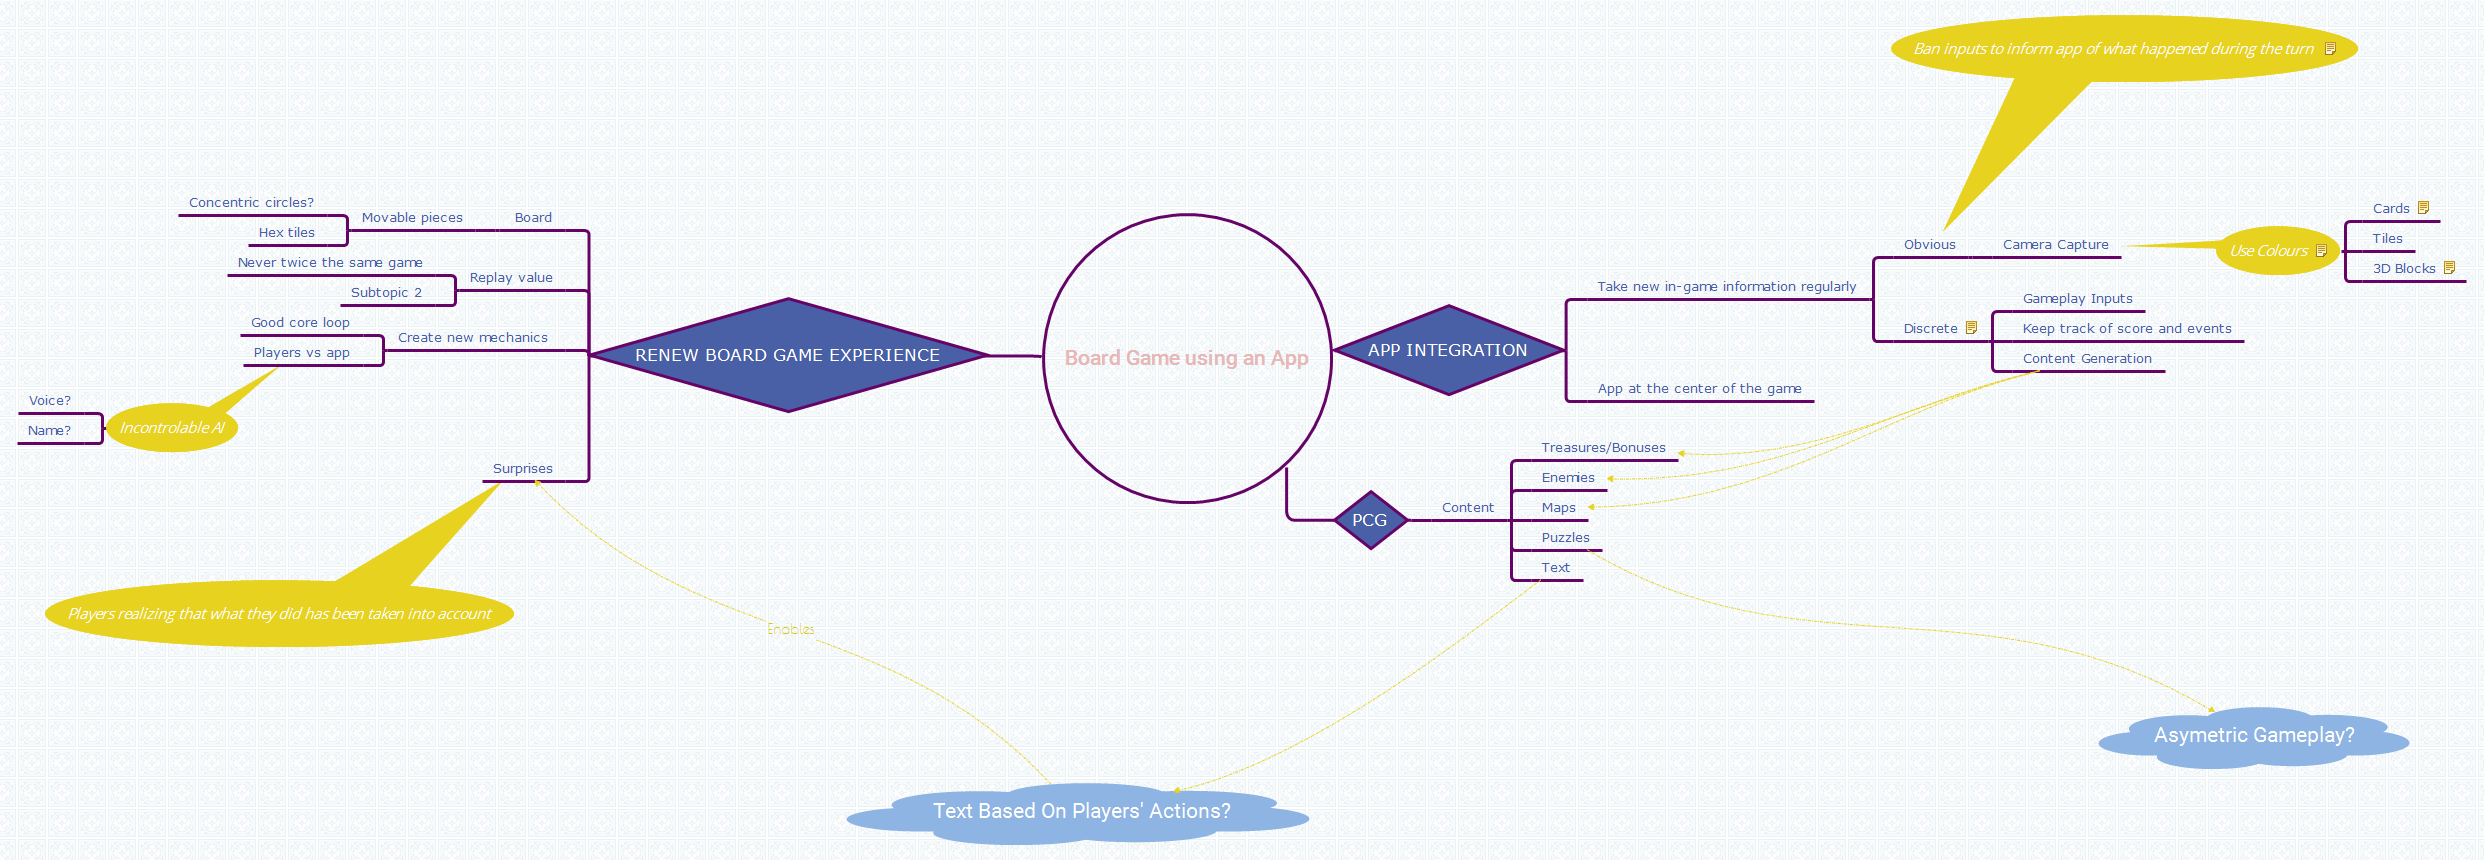
\includegraphics[scale=0.18,angle=-90]{Images/Brainstorm1.png}
    \caption{The first mind map exploring the ideas behind the PCG-based app integration in board games.}
    \label{fig:brainstorm1}
\end{figure}
\chapter{Second Brainstorm}
\begin{figure}[h]
    \centering
    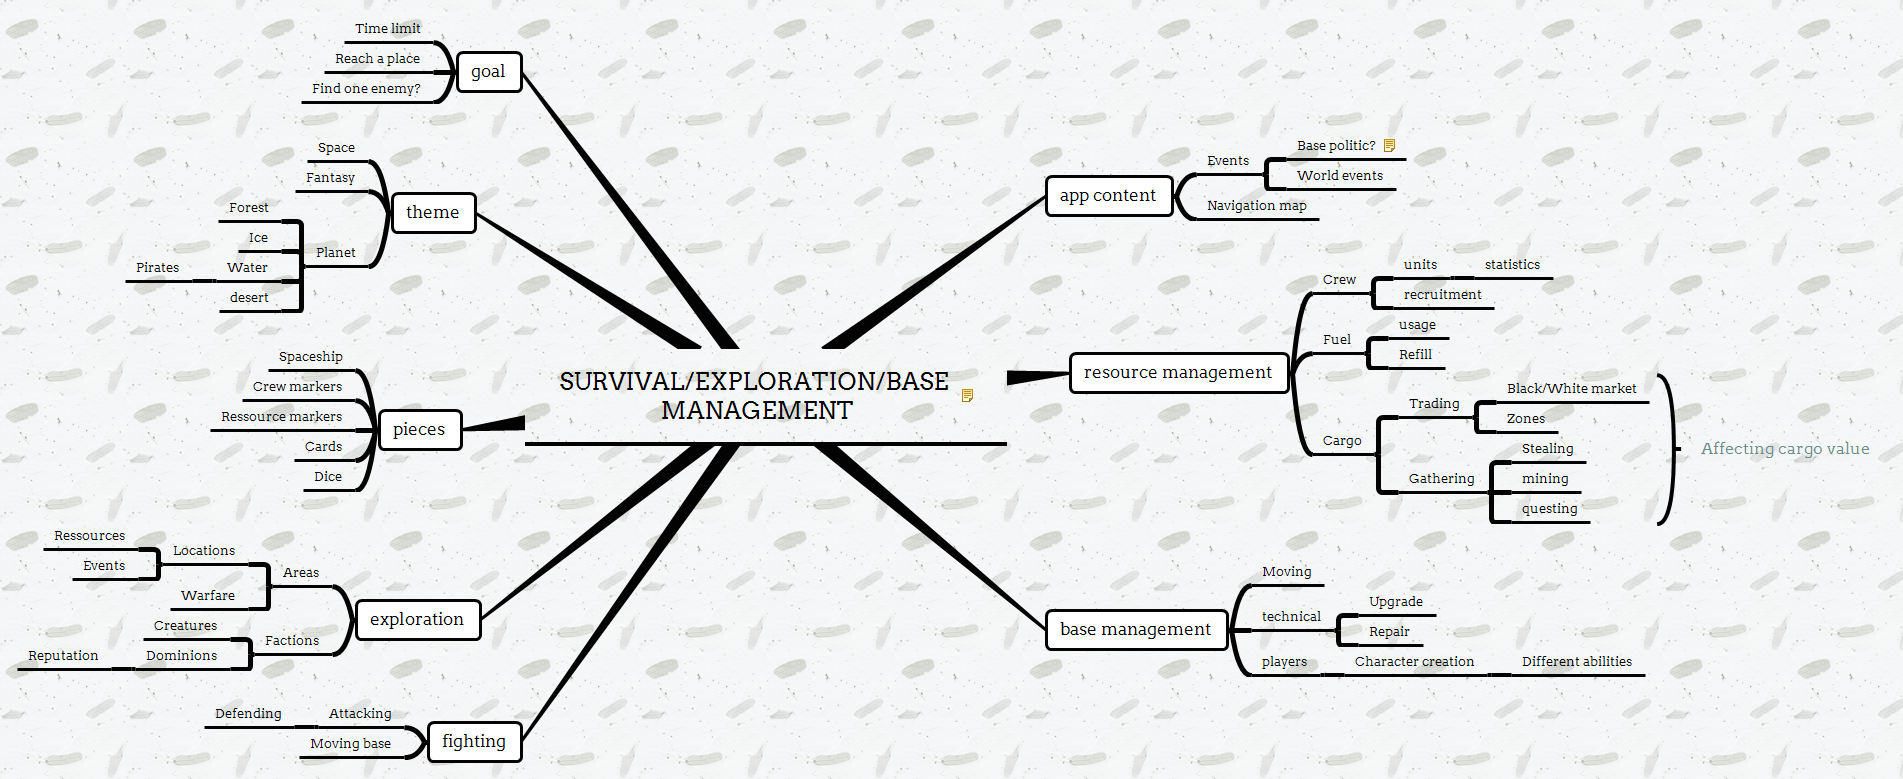
\includegraphics[scale=0.25,angle=-90]{Images/Brainstorm2.png}
    \caption{Mind map based on the core concept of exploring the different possibilities.}
    \label{fig:brainstorm2}
\end{figure}
\chapter{Digital implementation prototype}
\begin{figure}[!ht]
   \centering
   \begin{subfigure}[b]{\textwidth}
       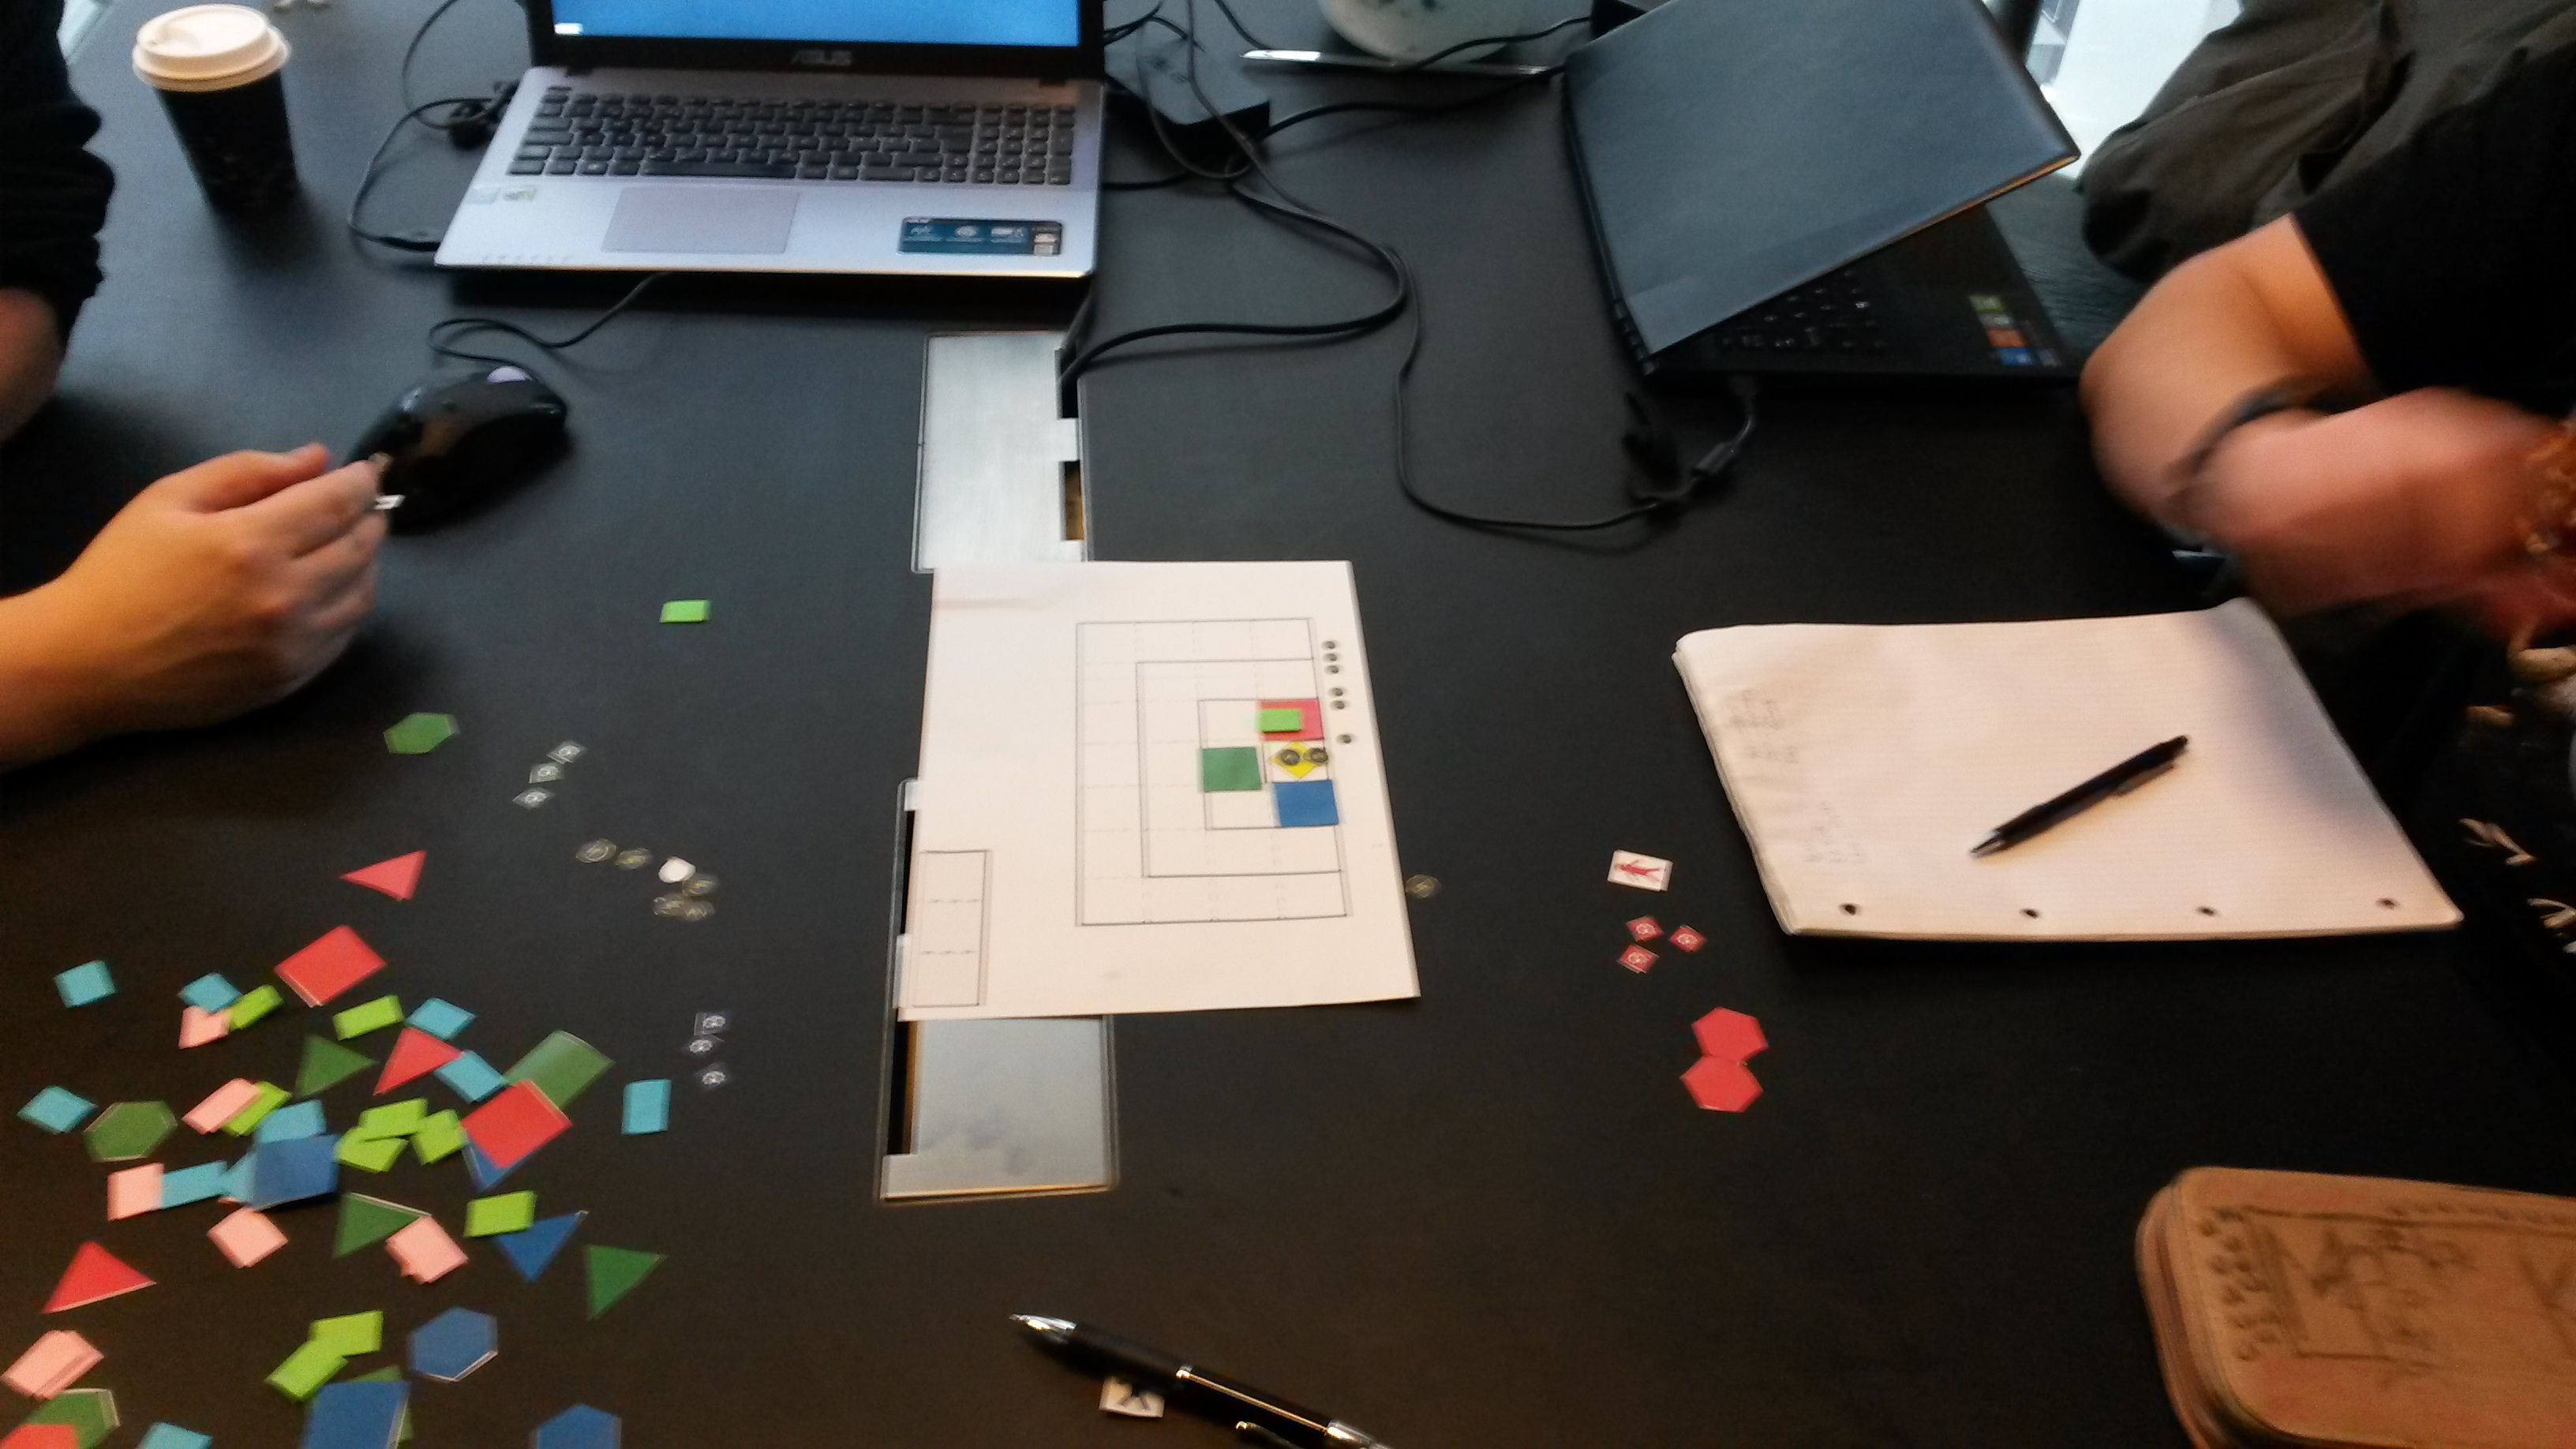
\includegraphics[width=\textwidth]{Images/proto2.jpg}
       \caption{Playtest based on another iteration of the board mechanics.}
       \label{fig:flowtest}
   \end{subfigure}
   \begin{subfigure}[b]{\textwidth}
       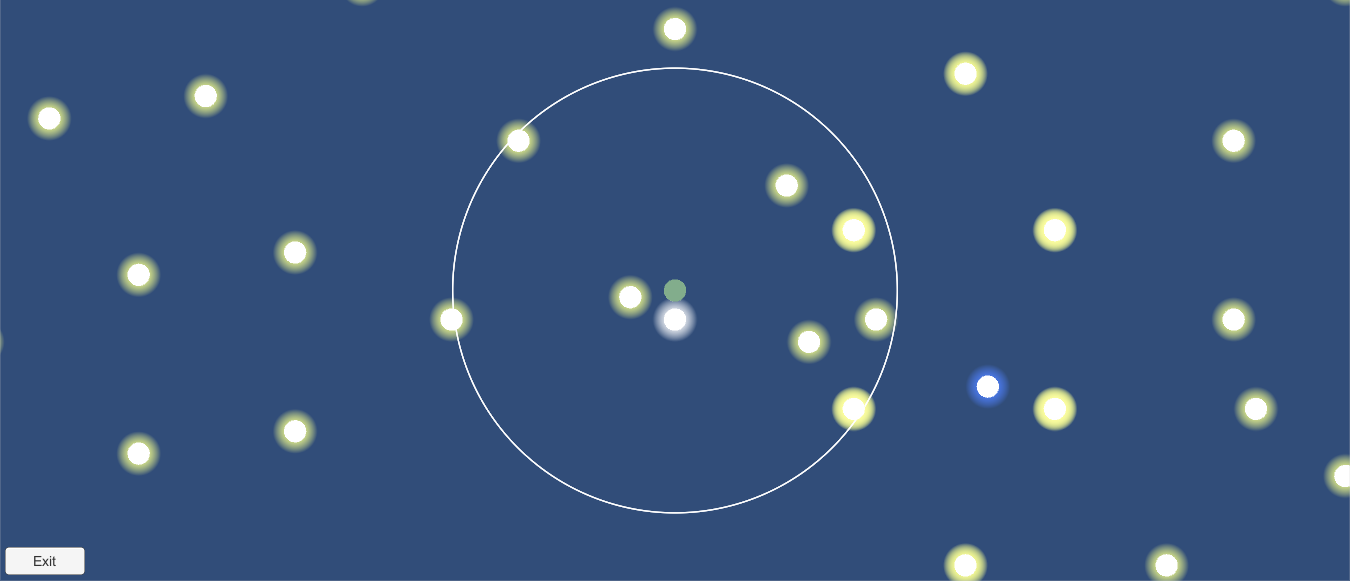
\includegraphics[width=\textwidth]{Images/proto2map.png}
       \caption{Map layout. The nodes do not contain the events, which are still simulated with dice roll.}
       \label{fig:flowmap}
   \end{subfigure}
   \caption{Testing the implementation of a digital component within the game flow.}
   \label{fig:gameflow}
\end{figure}

\chapter{High level walk through of the application}
\section{Generate Events}
\label{overviewapp}
In the world map, all the islands that were generated are being displayed. And when the player moves the castle to an island, i.e. goes to explore it, a new screen will be shown to the players, called the NodeScene. This screen is showing the island and the "explorable" locations on it. But before they can be displayed, they need to be built. 

\section{How an event is built}
An event is generated by selecting which type of event it is going to be; Gathering or Research. Both of these event types have 5 different location types affiliated with them. Mines, quarry etc. for the gathering, and Lake, forest etc. for the research. As soon as the event type is selected, a location is also selected. Now the algorithm goes into an XML file containing all the different rewards and conditions, and picks a number of them; 1, 2 or 3 different options that the players can select from. Associated with all the conditions used in the event, there are a list of possible outcomes that can happen if said condition is chosen, be it gaining resources or losing player tokens. The outcomes of every event are changed by the current standing the players have with the faction controlling the island the players are currently on. 
Once the options and outcomes have been generated, the location icons will be loaded to the island, and the players are free to choose which one they would like to explore.

\section{Moving around the world}
The main course of the game is to move from the start all the way to the goal node. But the castle can only move a certain length each turn. This means that the players will have to plan their way by looking at which island they can reach at any given time. The layout, however is made so that the castle that is being moved, always is able to reach at least 1 island each turn. If there are more than 1 island within the ring surrounding the castle (indicator for where they can move to), it is up to the players to choose where they want to go, and which direction to take. There is always the little arrow in the lower right corner of the screen, indicating which direction the final goal is. The players are always welcome to go back where they came from, and travel to already visited islands, though they will not be able to "re-explore" them. So should the players by chance start off going the wrong way, it does not ruin the game for them and make them unable to return.

\section{Interacting with the islands}
In order to travel to an island, you will have to click on the sprite image that is representing them on the world map. The island also has to be within range of the castle in order for any interaction to be possible. 
Once you click on the island, you will be greeted with a pop-up box that will ask you to confirm that you want to travel there. If this is the case, just hit the "travel" button, and the castle is on its way. If however you change your mind for some reason and wish to travel to another island, you can either move the viewport a little (click outside the box) or you can travel there, and go back later, or click the close button. If you click outside the box or the close button, the box will close, and you are free to select an alternative route.

When you have reached the island and the next scene is loaded, you will be able to choose from the possible variations of locations on the island. As mentioned before, there are a number of different types of locations, and each of them has their own look, feel, and purpose.
A location point is clicked on and as it is a sprite, the click has to be registered via raycasting. The touch on the screen has its location found, and a ray is then cast between the touch point and the world point within the application, and if the resulting ray goes through the sprite with the location attached to it, the event will begin. When the event begins, the possible options, outcomes, and the success indicator; good, bad or neutral and the rewards or penalties associated with them, will be presented to the user.

\section{Flavour text combinations and it's purpose}
Being a hybrid between a board game and a digital game, it is important that the players are presented with text that they can read in order to get into the feel of the game, and the setting in which it takes place. This means that there was a need for a lot of flavour text that will tell the players these things. 

Every island has a name and a short piece of text along with it. These texts are pre-made and are applied to the island when they are generated in the beginning. 
It is in the events that the real challenge is. The flavour text for the events needed to be linked with the location type, i.e. if the location type is a lake, the text needs to reflect that the area is a lake. So in order to make this happen, every location have a number of pre-made text strings associated with them, and one of those are selected as soon as the event is generated. On top of that, one of the bigger challenges was to have flavour for all the options, or buttons, that the players would be able to select from. The text needed to be based on what the players are using and it needs to be able to be combined with more text in case there is more than one board piece required for the option. The flavour also needs to be somehow connected with the type of location, so if you were at a lake and had to send out a castle crew, the text would say something like "send a crew down to the lake" instead of saying "send a crew to explore". The feel that it is connected and not just generic for everything, is important, as without it, one could just as easily have a deck of cards. 

Now that all the conditions have been "flavoured", the challenge moves on to the result-flavour. This is the flavour that is being shown as soon as an option is selected. It is constructed by combining strings of text that are based on the resulting rewards. So if you get 1 piece of Alchemical Material plus 1 crystal charge, the resulting finished flavour text would look something like "You found a new piece of material when you were exploring. As you enter the castle again you notice that within your findings, were a piece of shiny crystal". 
This concept goes for all possible combinations of result flavour. And each piece is selected from a variety of strings associated with each type of reward and penalty. By having all these pieces being able to be combined, we remove the need for having a huge bunch of cards on the table, as all the "cards" are being made procedurally. Also, we can just make more blocks of text and by doing so we are creating another deck of cards for each piece of text added.

The exact way the different flavours are combined is described in the event section above.

\section{Using memory to generate special event occurrences}

Special events is a feature that takes use of the fact that the application has memory. By checking the previous events, conditions and overall parameters within the data, we can compare the data and check how everything is connected. In doing so, we can make a list of conditions that needs to be met within an event, in order for a special event to be triggered and created. What we do as of now, is to have very specific requirements for an event to be able to trigger the special events. If the original event has a 3rd option, which is the "special" option, a check will be made to see if the overall conditions of the event check out in comparison to the list of special events.
For instance; a special event will be triggered if a preceding event was affiliated with the faction "Highbournes", and the location was a forest. Then the special event will occur on the world map X turns later, determined by a random initializer integer. When said special event then is triggered, it will use the data saved from the event that triggered it, and check which option was chosen, what the conditions for that option were, and then generate the text and result from that data.

All the resulting data is then also saved into the datamanager class, and the values are updated, e.g. the reputation with a faction increases/decreases, etc.


This concept of having special events being triggered and be based on already saved data is one that really separates this game from being just a board game, to being something of a more technological game. There are a lot of different ways this data can be used, and this is just one of them. More ways and our thoughts and ideas on this matter will be discussed in the discussion section.


\chapter{Game Rules}
\label{sec:rules}
%\includepdf[pages=1-10, angle=90, pagecommand={}]{rules.pdf}

\end{document}